\newcommand{\homedir}{/home/bscholtz/workspace/workspace-latex/2016-Design-Project/LATEX/}

%######################Preamble######################
\input{"\homedir preamble.tex"}

\newcommand{\coursecode}{EEE4036A}
\newcommand{\assignment}{Parking System Design Project\\Team 14}
\newcommand{\lecturer}{Riana Geschke}

\pagestyle{fancy}
\fancyhf{}
\rhead{Design Project}
\lhead{Team 14}
\cfoot{\thepage}

\begin{document}
\pagenumbering{gobble}
%######################Title Page######################
\begin{titlepage} 

\includegraphics[width = 17cm]{images/uctbanner.png} \\

\begin{center}
\begin{LARGE}
Faculty of Engineering and the Built Environment \\
Department of Electrical Engineering \\
\end{LARGE}
\end{center}

\begin{center}  
\begin{Huge}
\textbf{\coursecode}\\
\bigskip
\bigskip
\hrule
\assignment \\
\end{Huge}

\vspace*{\fill}

\hrule
\begin{center}
\textbf{Benjamin Scholtz (SCHBEN011)\\
Jarushen Govender (GVNJAR002)\\
Isaac Lebogang Khobo (KHBISA001)\\
Nasko Stavrev (STVATA001)\\}
4$^{th}$ year BSc. (Eng.) Electrical Engineering Department\\
Lecturer: \lecturer \\
\today
\end{center}
\bigskip
\hrule

\end{center}
\end{titlepage}

%######################Contents######################

\newpage
%\section*{Contents}
%\addcontentsline{toc}{section}{Contents}  
\tableofcontents

%######################Plagiarism Dec.######################
\input{"\homedir plagiarism-declaration.tex"}
\pagenumbering{arabic}
%######################Begin Content######################
\newcommand{\lsec}[1]{\normalsize{\textbf{#1}}\\}

\newpage

\section{TASK CLARIFICATION}
\subsection{Background}
UCT Upper campus has a number of parking areas for staff, students and visitors using cars to travel to campus. There are red, yellow, blue/unmarked bays on campus. In addition there are disabled and 
visitor parking bays on campus. These categories are assigned the highest priority. 

For every user, a parking category is assigned, and an associated annual fee is charged.  The purchase of a parking disk allows the staff member/student/visitor to search for a parking spot in the designated category on campus, but it is not guaranteed that one will be available, since parking bays are oversold. When arriving on campus, a driver of a car may spend some time searching for an available spot in the required category. Parking disks are generally linked to a person and only valid for the specific vehicle for which the disk has been purchased, except for student lift clubs.

The Traffic  Department  on  Upper  Campus  administrates  and  manages  all  aspects  related  to  parking  of vehicles.\cite{assignment}

In the figure below a survey of UCT students was completed to determine of those students who owned a blue parking disk, how many of them would park illegally in the case of there being no more blue parking bays on upper campus. The results clearly indicate that illegal parking is a problem with the current UCT parking system.

\begin{figure}[H]
\begin{center}
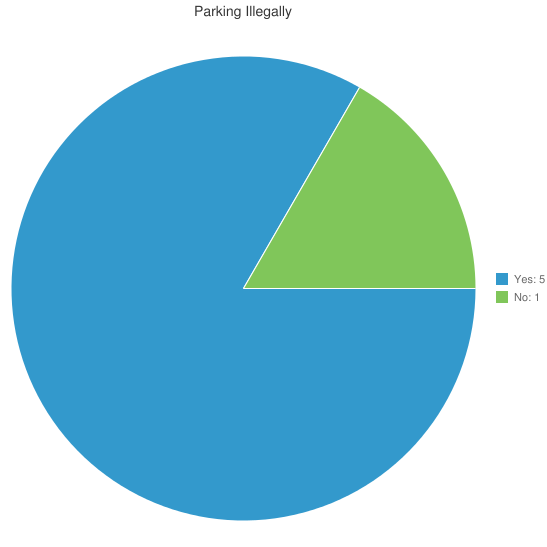
\includegraphics[scale=0.55,clip]{data/chart.png}
\caption{Illegal parking on UCT upper campus.}
\end{center}
\end{figure}
 
\subsection{Problem Statement}
For  a  driver  entering  Upper  Campus  in  a  car,  it  is  not immediately  apparent  where  there  are  parking bays available.  This is a particular problem during peak times when a large number of cars arrive on campus, looking for parking at the same time. The second problem that exists is that these users then choose to park illegally if a parking bay can not be found (as shown in the figure above). The design assignment is to solve this problem using the electrical engineering skills of each of the team members in our group.\cite{assignment}

The design assignment is:

\begin{itemize}
\item To provide information in an easily accessible format, to each driver of a car immediately on arrival on campus, on where all the vacant parking bays on campus are. This must be for the specific category of parking for this user.

\item To determine whether a vehicle is parked on a bay not designated for this user, for example a yellow disk holder parks on a red bay, or a visitor parks on a disabled parking bay, and make this available to the traffic department in real time.

\item To  allow electronic reconfiguration  of  traffic  bay allocations  on  special  occasions, for example during the summer school period, when there are many visitors requiring parking on campus.

\item To monitor and log the use of parking bays and the percentage of occupation of each parking area and make this available to the traffic department, for the purpose of planning.\cite{assignment}
\end{itemize}

\newpage
\section{CONTEXT OF DESIGN}
\subsection{Macroeconomic Factors}
\subsubsection{Technical} 
In South Africa there are a number of technical concerns to deal with regarding the production of electronic systems. The PCB design standards in South Africa are not of as high a standard as in certain overseas production houses and may have longer production times. The system might take a specialized skill set to maintain and repair the system components. Both of these factors need to be dealt with to achieve a balance between quality, production time and capital outlay for the system.

\subsubsection{Economic}
The current South African economy lends itself to local production of goods using cheaper local labour. The problem with local production is that it is still expensive to import the components and materials needed for the production - this can be justified considering that there may be a possibility to export any products developed as the economy lends itself to the export of goods to foreign markets. 

\subsubsection{Ethical}
A few ethical issues arise as soon as people or vehicles are equipped with electronics capable of tracking or logging movement and actions. Users will have to be made aware of the risks or lack there of. Legal advice will need to be used to draw up user agreements for the system. The ethics of tracking users will need to be considered and systems put in place to ensure users can not be tracked off campus, and that the data collected on campus is securely encrypted or stored.

\newpage
\subsection{Microeconomic Factors}
\lsec{UCT Parking Cash Flow}
To calculate the upper campus UCT parking cash flow in the table below, a few assumptions were made. Approximately 2.8 parking discs are allocated per bay. Assuming this is true of all parking bay categories, this results in a total cash flow of R13.6 million per year. Assuming that 20\% of this cash flow is used for maintenance, and the other 20\% for parking staff salaries, we are left with R8.16 million for the project, with possible external funding if necessary.

The following table shows the number of different privilege level parking spots  and what the user pay for those slots, as well as how many users are allocated to those spots in order to calculate the cash flow acquired from the user yearly disc payments.

\begin{table}[H]
\centering
\caption{Upper Campus UCT Parking Cash Flow}
\label{cash-flow}
\begin{tabular}{lllll}
                         & \textbf{Parking Bays} & \textbf{Allocated Bays} & \textbf{Disc Price (R)} & \textbf{Cash Flow (R)} \\
\textbf{Red}                      & 808                   & 2262.4                  & 1524                & 3447897.6          \\
\textbf{Yellow}          & 1046                  & 2928.8                  & 960                 & 2811648            \\
\textbf{Student}         & 2757                  & 7719.6                  & 960                 & 7410816            \\
\textbf{Total Bays}      & 4611                  & 12910.8                 &                     &                    \\
\textbf{}                &                       &                         &                     &                    \\
\textbf{Discs/bay}       & 2.8                   &                         &                     &                    \\
\textbf{Total Cash Flow} & R13670361.6            &                         &                     &                   
\end{tabular}
\end{table}

From the table above and with with calculated R8.16 million available for research and development, the project capital expenditure should be below R5 million - this leaves enough capital for unforeseen expenses, either from oversight or incurred risk.

\lsec{Social Behaviour}
UCT parking system users are currently forced to take illegal action when locating and using parking bays due to a lack of parking bays available. The new system will have to address these issues and the mindset of the parking system users will have to change to accept the new system that will introduce more red tape and make it harder for them to get away with parking illegally. This could be addressed by having a parking system that adjusts to the regularity at which a user parks and charging them accordingly - this will motivate users, even if they are in possession of a disk, to find other means of transport on certain days, thus reducing the parking system load.

\newpage
\section{DESIGN SPECIFICATION}
\subsection{Scope}
This specification covers the analysis, design, production timeline and considerations, and lifecycle of the upgraded UCT parking system. The specification is for a parking system on upper campus to be used primarily in allocated parking zones rather than dispersed parking bays. The parking system specifications aim to meet the requirements introduced in the client problem statement.

\subsection{Applicable Documents}
The following documents are applicable to the project and are of importance to the ultimate specifications of the project:
\begin{itemize}
\item Group Allocation
\item Group Project Assignment
\item Design Notes
\end{itemize}

\subsection{Characteristics}
\subsubsection{Functional Characteristics}
\lsec{Function 1: User interface} 
Information must be available in an easily accessible format to indicate to drivers where legal parking bays are located.

\lsec{Function 2: Vehicle location}
Real time location and classification of vehicles in UCT parking areas based on user parking privileges. 

\lsec{Function 3: System back-end}
Traffic department should be able to access data about vehicles and users on a database as well as reconfigure traffic bay allocations. The use of parking bays should be monitored and logged to be processed to show percentage occupation of parking area and get historical data.

\lsec{Interface Characteristics} 
Function 1, 2 and 3 should be linked with a wireless communication method.

\newpage
\subsubsection{Quality Assurance}
\lsec{Standards and Codes}
The design must meet the following standards and codes:
\begin{itemize}
\item IEEE Standards.
\item SABS Standards.
\item ICASA RF Regulations.
\item RF PCB Design Standards.
\end{itemize}

\lsec{Methods of Testing}
The design should be tested using the following method:
\begin{enumerate}
\item Periodic random parking bay testing.
\item HIL system testing.
\item Brute force user and operator interface testing.
\item Long term power system testing.
\item RF propagation testing.
\end{enumerate}

\lsec{Reliability Issues}

Reliability issues will arise in the following forms:

\begin{itemize}
\item Component quality standards.
\item Supplier reliability (especially for importing).
\item User familiarity with the system.
\item Unknown environment variables (RF signal propagation, mechanical obstructions etc.)
\item Unknown user variables (User behaviour etc.)
\end{itemize}

\newpage
\subsubsection{Timescale}
\lsec{Design Schedule}
The embodiment design should be completed within the given period of just under two months, in time for hand in after the first UCT term.

\lsec{Development Schedule}
Thereafter the final design should be developed and tested within a period of 4 months; and certified with the relevant organisations within a period of 2 months.

\lsec{Production Schedule}
The final design should be prototyped over a period of 1 month and then any necessary changes completed within 1 month thereafter - a final product will be sent for production over the course of 1 month. The necessary traffic department staff training and student/user familiarisation will be completed during the production time period over a period of 2 months.

\lsec{Delivery Schedule}
The complete system will be installed and in use over the period of 1 month. 

\begin{figure}[H]
 \begin{ganttchart}[x unit=10mm, y unit chart=0.8cm]{1}{12}
\gantttitle{\textbf{Year of Implementation (months)}}{12} \\
\gantttitlelist{1,...,12}{1} \\
\ganttgroup{Design Schedule}{1}{2} \\
\ganttbar[bar/.append style={fill=yellow}]{Embodiment Design}{1}{2} \\
\ganttgroup{Development Schedule}{3}{8} \\
\ganttbar[bar/.append style={fill=blue}]{Final Design}{3}{6} \\
\ganttbar{Certification}{7}{8} \\
\ganttgroup{Production Schedule}{9}{11} \\
\ganttbar[bar/.append style={fill=blue}]{Prototype and Testing}{9}{9} \\
\ganttbar{Final Changes}{10}{10} \\
\ganttbar[bar/.append style={fill=blue}]{Final Production}{11}{11} \\
\ganttbar[bar/.append style={fill=red}]{Training and Familiarisation}{9}{10} \\
\ganttgroup{Delivery Schedule}{12}{12} \\
\ganttbar[bar/.append style={fill=red}]{Installation}{12}{12} \\
%\ganttmilestone{Milestone}{11} \ganttnewline

\ganttlink{elem1}{elem3}
\ganttlink{elem3}{elem4}
\ganttlink{elem4}{elem6}
\ganttlink{elem6}{elem7}
\ganttlink{elem7}{elem8}
\ganttlink{elem2}{elem9}
\ganttlink{elem8}{elem11}
\end{ganttchart}
\caption{Project Gantt Chart.}
\end{figure}

\subsubsection{Economic Factors}
\lsec{Market Analysis}
The users of the system will be predominantly students and a small number of staff who may have limited funding for parking disks. The cost of the disks need to be kept at the same price as outlined in the Microeconomic Factors, while adding the advanced functionality needed to meet the design specifications. On questioning users, they responded that they would not be willing to pay more for this advanced functionality - with some saying they still believe the costs for parking on campus are too high considering the lack of available parking on most days. The new parking system should address the above issues.

\lsec{Design Costs}
The design costs will be kept to a minimum by using UCT Electrical Engineering students to complete the design as a part of their EEE4036A design course.

\lsec{Development, Manufacturing, Distribution Costs}
The main costs incurred will be in contracted manufacturing and distribution. 

The following companies will be contracted to:
\begin{enumerate}
\item Zytek will be used for the manufacturing and assembly of the PCBs.
\item Skeg product development will be used for the tag and beacons casing production using injection mould methods.
\item Electronic components will be imported from Mouser predominantly. 
\end{enumerate}

The costs of development, manufacturing and distribution through the above sources should be kept to a unit cost value of less than R400 per tag. This ensures the cost of a disc will cover the cost of production of the tag, assuming  the allocation of funds as outlined in the Microeconomic Factors, with 60\% being left for hardware and software costs.

\subsubsection{Ergonomic Factors}
\textit{\textbf{Device definition:} in the following sections a device refers to whatever user interface and necessary user interactions, whether with software or hardware, are required for the parking system.}

\lsec{User needs}
The user should be able to easily use the interface, whether internal (cellphone app etc.) or external (LED sign board) while driving. The use of the system should not endanger the user by distraction or otherwise. The device should not interfere with the users field of vision.

\lsec{Ergonomics}
The ergonomics of the device should meet the needs of the user. The interface should be easily accessible. The process of installing the device in the car should be self explanatory and not involve a complex process that requires assistance from UCT parking staff.

\newpage
\lsec{Controls}
The controls of the device should meet the needs of the user. The controls should be minimal to avoid complexity and distraction, yes should also allow access to all the functions as set out above in the Functional Characteristics section.

\subsubsection{Life-cycle}
\lsec{Distribution}
Distribution of the device should be on a yearly basis, with user returning the device for maintenance and license renewal.

\lsec{Operation}
The user should be able to install the device easily and have it operate reliably for the period of one year. 

\lsec{Maintenance}
Minimal maintenance (whether for power source or mechanical maintenance or UID configuration) should be required for the device, with a minimum maintenance cycle of one year which is the period a user will be in possession of said device and expect it to operate reliably. Realistically this mean the maintenance cycle should be at least two years for worst case design - this will lessen the risk of a failure during the one year cycle.

\lsec{Disposal}
The device and it's components should, if required to be, be disposed of in a safe manner - this includes batteries and any other harmful substances. The device, after one year of use, should be returned to the parking staff especially during the initial testing phase where the system will be reviewed. The entire system should be operational for a period of at least 15 years. This will ensure that the system makes a return on investment.

\subsection{Acceptance Test Requirements}
\lsec{Function Test Requirements}
The following tests will be put in place to ensure the system meets the functional specifications outlined above before and during the system's operation:

\begin{itemize}
\item \textbf{In-service measurements:} Permanent disk installation (either RFID, Decawave or otherwise) to have a way of testing each parking area is operating correctly without relying on a user reporting the issue.
\item \textbf{Manual inspection:} Weekly inspection during non-peak hours, to randomly test various bays in each section.
\item \textbf{Field trials:} Trial the system in a low-traffic parking area before users are introduced to the system for the first time.
\end{itemize}

\newpage
\section{CONCEPTUAL DESIGN}
\subsection{Design One}
Design One (D1) uses a triangulation system to locate the registered vehicle within the parking area. Each registered vehicle has a tag with a unique ID - this ID has the user data linked to it in a database on the server back-end. The location of each parking space is known, and with the knowledge of where the vehicle is located it can be determined whether the vehicle is legally parked or not. 
  
\subsubsection{System Diagram}
Figure~\ref{fig:soft-overview2} below shows a diagram detailing the overall structure of the system. 

\begin{figure}[H]
\begin{center}
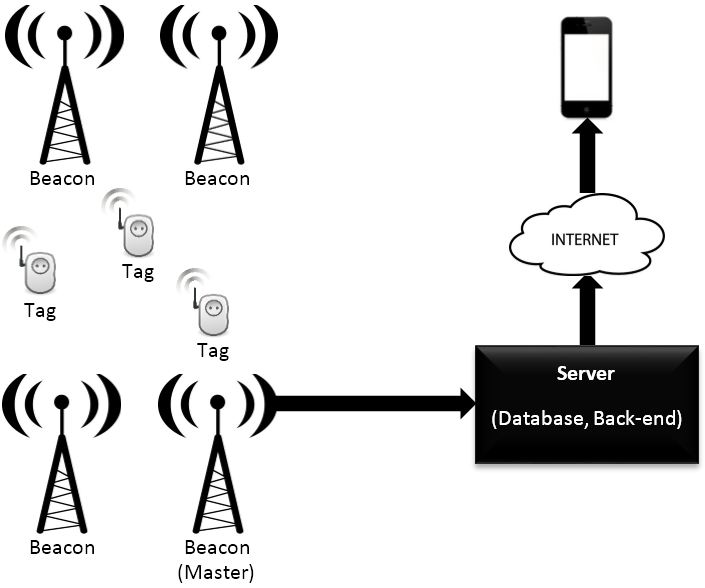
\includegraphics[scale=0.5]{data/software/1.jpg}
\caption{System overview.}
\label{fig:soft-overview2}
\end{center}
\end{figure}

The system uses trilateration to locate the parking system users, relay this information to a server for processing and supply the necessary parking information to the user via a mobile or web interface. This will be further expanded upon in the System Components section.

\subsubsection{System Components}
\lsec{Tags and Beacons}
Due to a triangulation system being used, in every parking area there are at least three beacons - with four being used to try to eliminate signal propagation issues. The tags and beacons make use of a Decawave DW1000 ultra-wideband transceiver chip that is controlled via SPI from a Atmel micro-controller. 

The master beacon sends a signal out to synchronise all the beacons to the same time reference. Each tag sends a signal periodically with the unique user ID, transmit time and battery level which is received by each of the beacons. The beacons all relay time of flight data back to the master beacon which performs a time difference of arrival (TDOA) calculation to determine where the tag is located.\cite{decawave-presentation}

The tags transmit with a period of 5-10 minutes. This reduces power consumption and signal noise level interference with other tags. The tags do not receive data. The tags will be accurate to within 10cm giving more than enough accuracy for the application. The initial conservative battery life estimate is 5 years with proper power management in software. They will be powered with a LiPo battery that will need to be replaced or charged when discharged.

The beacons will use the same circuitry, but with different software running on the Atmel micro-controller. They will be required to both transmit and receive. The beacons will be mounted on poles (both light and installed) distributed across the UCT campus - this will allow the location of vehicles in any area. They will be powered with LiPo batteries which will be charged with solar panels - or wired in cases where this is not practical.

\lsec{Server Back-end}
The server back-end connects with the master beacon via WiFi and receives the tag location, unique ID and battery level for every new vehicle. This is updated on a database every 5-10 minutes. Further calculations and visualizations are performed and stored in the database to send to the end user. The following data will be available for each unique ID:

\begin{itemize}
\item User privileges.
\item Tag location (updated periodically).
\item Tag battery level (updated periodically).
\end{itemize}

\lsec{User Interface}
The user interface will connect with the server back-end to access the database and will relay the following data to the end user via a smart phone application or web application: 
\begin{itemize}
\item Indication of privilege level and violations.
\item Tag battery level.
\item Vehicle location.
\item Location of open parking bays.
\item Recommended parking area.
\item Number of free parking bays in parking area.
\item Traffic heat-map on campus.
\end{itemize}

\subsubsection{Requirement Satisfaction\cite{assignment}}
Design One satisfies the design requirements outlined in the Task Clarification section in the following ways:

\begin{itemize}
\item \textbf{To provide information in an easily accessible format, to each driver of a car immediately on arrival on campus, on where all the vacant parking bays on campus are. This must be for the specific category of parking for this user.}\\
Design one satisfies this requirement by not only tracking parked vehicles and where they are, but also the user entering UCT upper campus - this allows the mobile and web GUI system to give user specific directions to the nearest available parking bay.

\item \textbf{To determine whether a vehicle is parked on a bay not designated for this user, for example a yellow disk holder parks on a red bay, or a visitor parks on a disabled parking bay, and make this available to the traffic department in real time.}\\
Each bay will have it's corresponding GPS coordinate in the database. Every car with a disk on campus will be tracked, which means that whenever someone illegally parks the UCT parking department will know. Visitors will have to be allocated visitor discs for the system to work for all cases.

\item \textbf{To allow electronic reconfiguration  of  traffic  bay allocations on special occasions, for example during the summer school period, when there are many visitors requiring parking on campus.}\\
The database will be easily reconfigured to allocate each GPS parking location to a different category of user. Visitors will have to be allocated daily disks, much like they are currently required to do.

\item \textbf{To monitor and log the use of parking bays and the percentage of occupation of each parking area and make this available to the traffic department, for the purpose of planning.}\\
Not only will the design be able monitor and log the use of parking bays and parking areas via the database, the traffic department will be able to see both real-time movement and post-processed heat maps of campus and where cars are located.
\end{itemize}

\subsubsection{Evaluation}
\lsec{Cost} 
The cost of installation of the system will be minimal with the decisions made for costs to be incurred in the distribution of the tags rather than permanent hardware.

\textit{Implementation}\\
The implementation of the system will be very efficient, as very little permanent mechanical installations exist. Implementation will involve distribution of the tags and the set up of the server back end. The poles for the beacons will be easily installed. 

\newpage
\textit{Maintenance}\\
Maintenance will involve ensuring all tags are working optimally on a yearly basis. The tags are estimated to last on a single 1000mAh LiPo for a period of 3 years. The beacons will most likely need very little maintenance, as they are only subject to weathering and not mechanical impact of vehicles. 

\textit{Energy Consumption}\\
As with the tags, the beacons are also very power efficient, with minimal circuitry and a low density per parking area. The tags are an insignificant energy cost. The beacons will run on solar energy, as they can be trickle charged without having to have solar energy every day.

\lsec{Strong/weak Points}
Strong:
\begin{itemize}
\item Low energy usage.
\item Minimal installation effort and costs.
\item Minimal maintenance effort and costs.
\item Low cost system overall.
\item Extensive location information from post-processing.
\end{itemize}

Weak:
\begin{itemize}
\item Relatively expensive tag in high risk environment.
\item Possible RF interference.
\end{itemize}


\subsubsection{Risk Assessment}
\lsec{External Causes} 
Human Interference \textbf{(high risk)}: The users of the system play a big role in the RF performance of the system - the users need to place the tag on the window of the vehicle in order to ensure there is minimal interference from the car body, if the user fails to do this then the system could fail for that user. The tags are relatively expensive, and could be a target for theft.

Weather \textbf{(low risk)}: The intended lifetime of the beacon and tag system is 15 years. Cape Town receives high wind speeds and rainfall - this poses a relatively large risk to the beacons. UV sun damage poses a risk to the housing of the tags, which will be exposed on the windscreen of the vehicle. 

\lsec{Internal Causes}
Failure to recognize long-term design flaws \textbf{(low risk)}: The system is well documented and simple in terms of implementation and maintenance. The risk of long term design flaws lies mainly with the power source of the tags and the RF design of the system. There could also be design issues in the UI that could cause confusion in managing the system.

\newpage
\lsec{Mitigation}
The following steps will be taken to mitigate these risks:

\begin{enumerate}
\item Proper marketing to users and training to staff will be provided prior to the system's installation - this will ensure proper use of the system.
\item Assisted installation of tags for first time users.
\item Proper material engineering design and waterproofing will be implemented to ensure endurance to weathering.
\item Costs will be reduced by eventually manufacturing the product overseas, the tags will also be made low profile to reduce risk of theft.
\item The system will be made modular which means that if one component fails the system continues working. 
\item There will be more than the required number of beacons in each parking area to ensure that if one fails the system continues working and if RF interference comes up, it isn't an issue.
\end{enumerate}

\newpage
\subsection{Design Two}
Design 2 (D2) uses radio frequency identification (RFID) to track the positions of vehicles. An RFID coil-pad would be placed on each parking bay and users would be issued a tag when they register for parking. This tag would make use of passive RFID - using radio energy transmitted by the reader instead of a battery – in order for the driver to be identified.

\subsubsection{System Diagram}
\begin{figure}[H]
\begin{center}
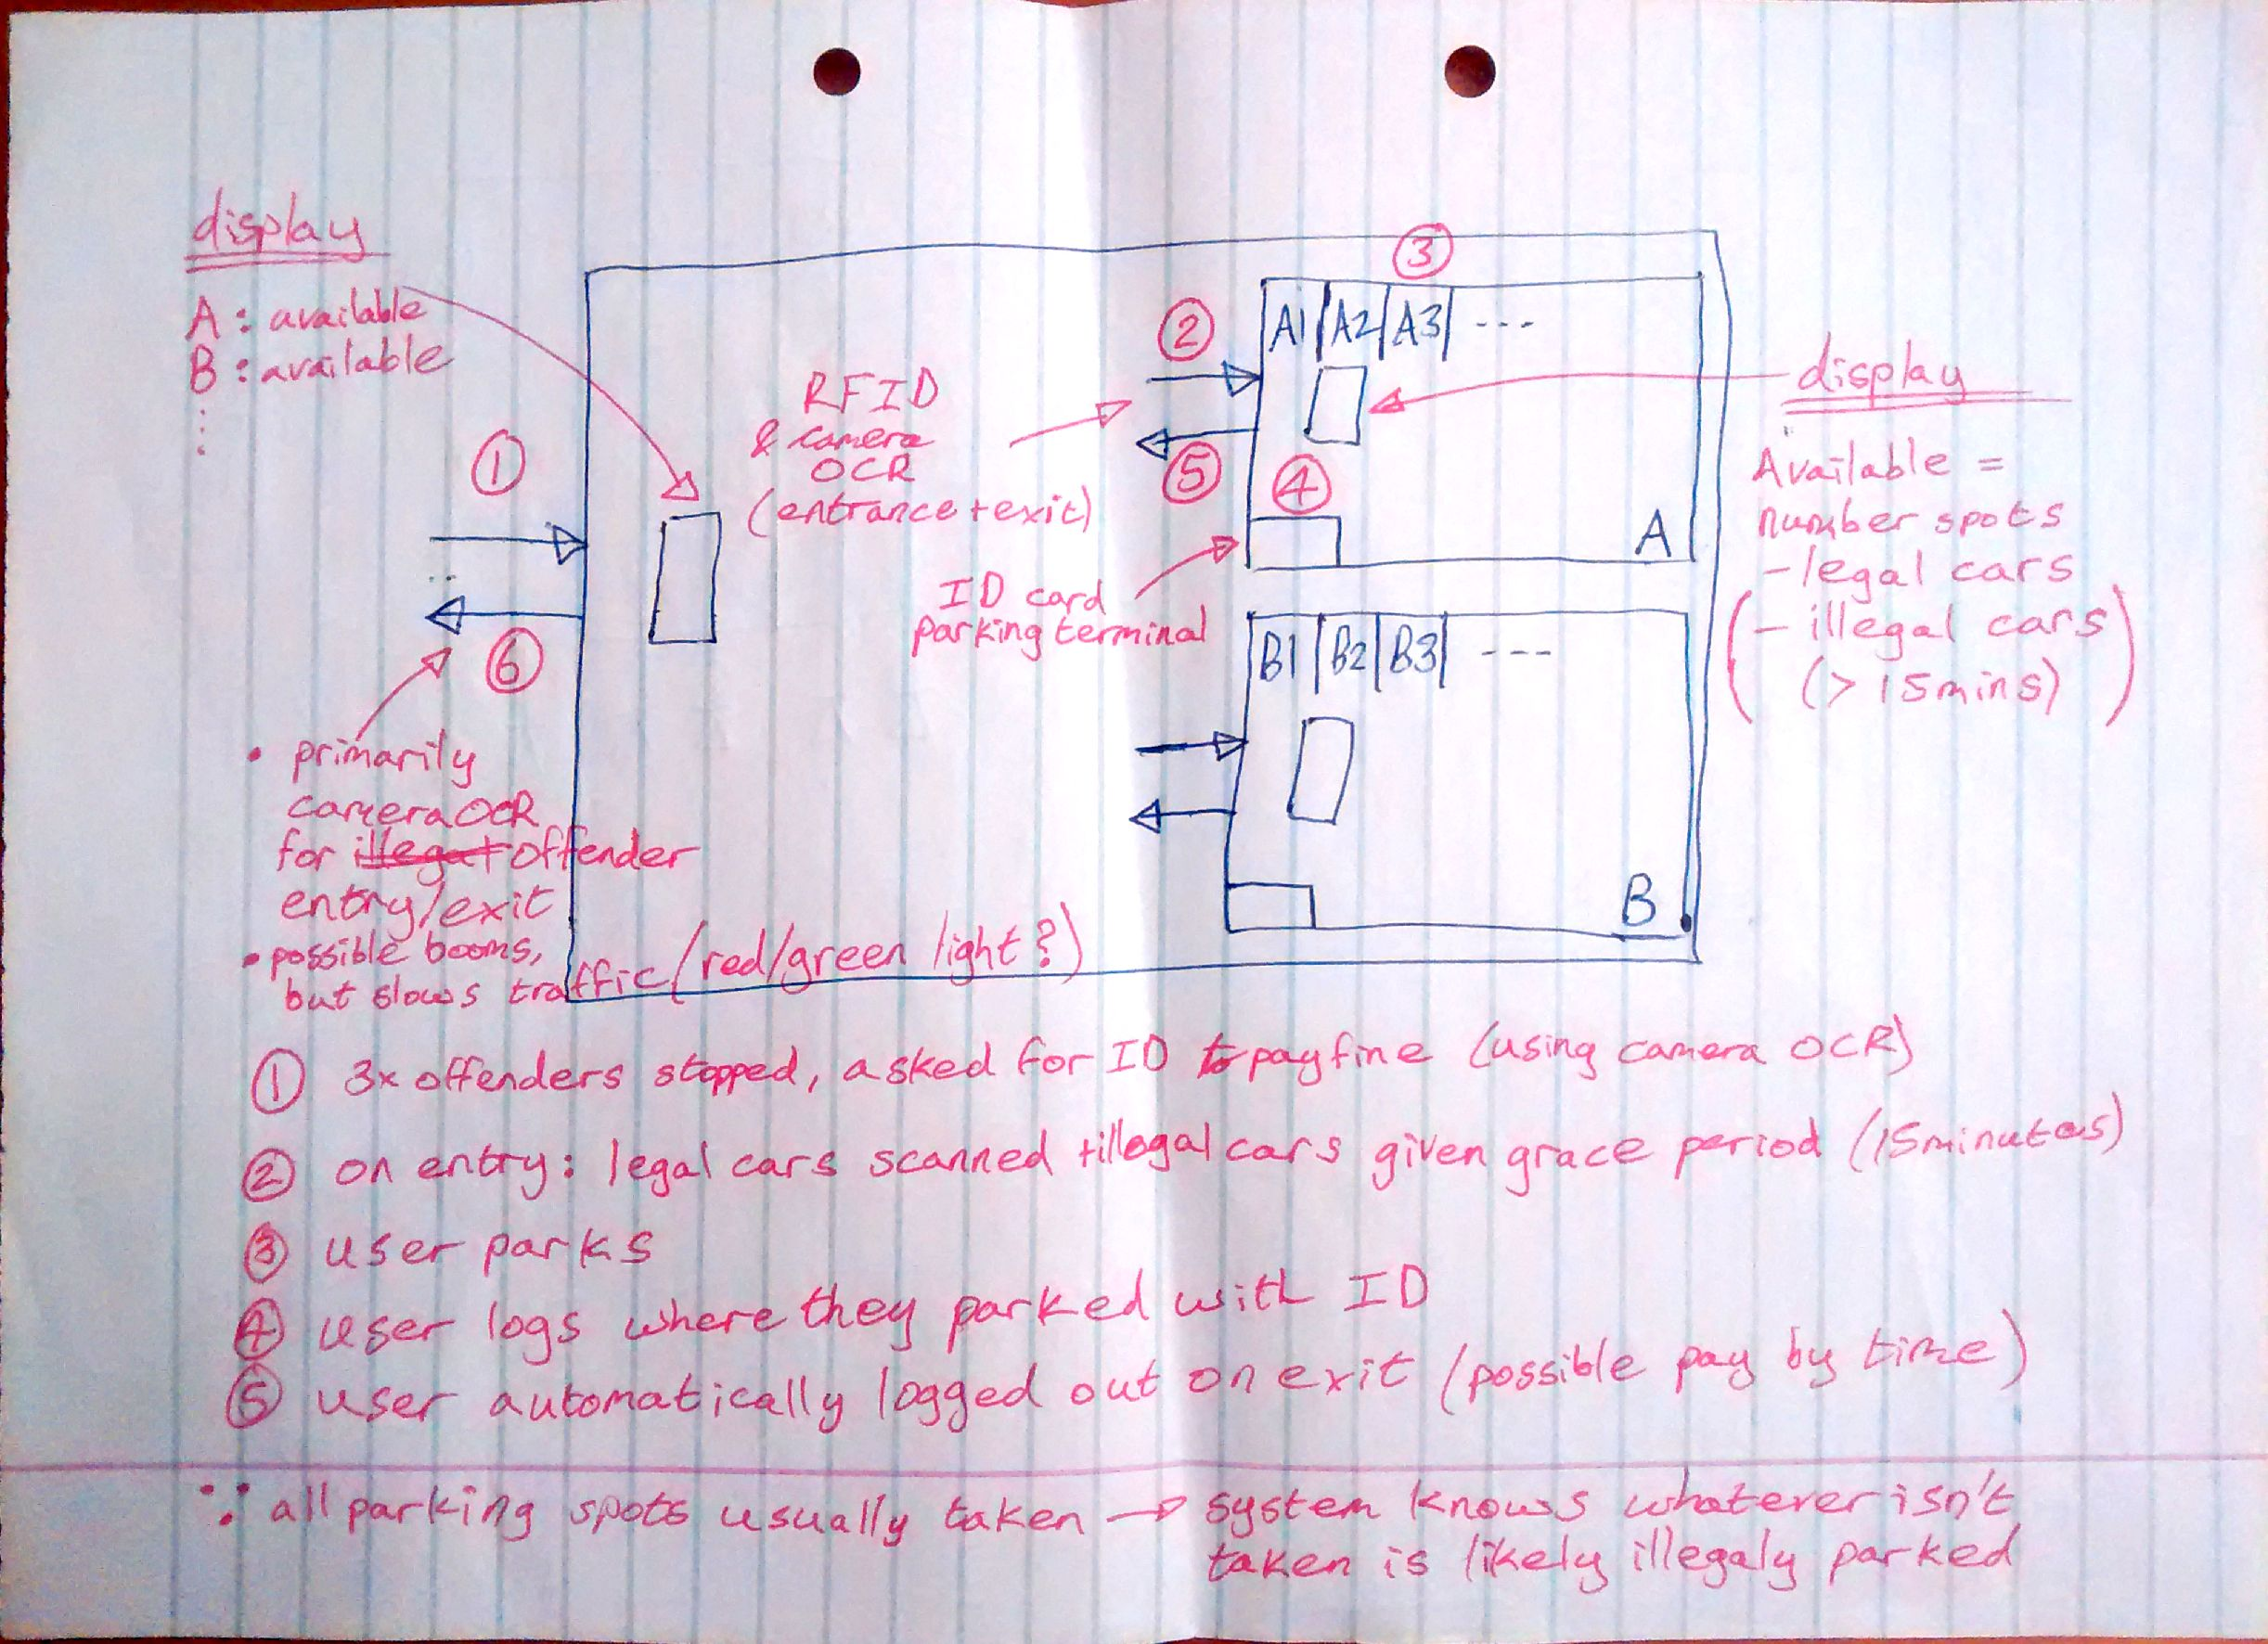
\includegraphics[scale=0.13]{data/D2.jpg}
\caption{System overview.}
\label{fig:soft-overview2}
\end{center}
\end{figure}

\subsubsection{System Components}
\lsec{RFID Tag}
Every user is issued with an RFID tag upon registration for parking at UCT. This will replace the
standard disks that are currently issued and users will be required to keep the tag in their cars at all
times. RFID tags can be either active, passive or battery assisted passive. Our tags will be passive in
order to save costs.

RFID tags contain an integrated circuit (IC) to store and process information as well as modulation
and demodulation procedures of radio frequencies, and the collection of DC power from incident reader signals. There is also an antenna usually which receives and transmit the required signals. Tag
information is stored in non-volatile memory.

\lsec{RFID Reader}
Readers transmit an encoded signal in order to identify the tags. When the tag receives this signal it
will respond with its identification. In our case, this will be a unique tag serial number in order to
identify individual drivers. Since tags have individual serial numbers, the reader is capable of
differentiating between multiple different tags that all within range.

RFID systems are usually classified by the type of tag and reader used. In our case it will be an Active
Reader/Passive Tag System, which will be transmitting identifier signals and receiving authentication
replies from the (passive) tags.

Tags which operate on Low Frequency and High Frequency bands are very close to the reader
antenna because they are actually only a small percentage of a wavelength away. In this area, the
tag is coupled electrically with the transmitter in the reader and can then modulate the field
produced by the reader by changing its electrical loading. By switching between lower and higher
relative loads, the tag produces a change for the reader to detect.

\lsec{RFID Sensor/Coil}
An RFID coil will be placed on each bay. This essentially will act as the readers antenna and will allow
information to be transmitted and received. The coil will be made of copper and be able to operate
in the required voltage band.

\lsec{Server Back-end}
The RFID active reader will connect back with the master via WIFI, relaying all important
information. This will include the bay used and the driver ID. This will be updated on a centralised
database roughly every 5-10 minutes. Other information will be able to be calculated or derived. The
following data will be available:

\begin{itemize}
\item User privileges (visitor, staff, student etc)
\item Tag location (updated periodically).
\item Bay occupation
\end{itemize}

In addition intelligent parking suggestions will be made to the user, based on the above mentioned
data. This is similar in principle to designs adopted by the parking facilities at many shopping malls.

\lsec{User Interface}
The user interface will connect with the server back-end to access the database and will relay the
following data to the end user via a smart phone application or web application:

\begin{itemize}
\item Indication of privilege level and violations.
\item Vehicle location.
\item Location of open parking bays.• Recommended parking area.
\item Number of free parking bays in parking area.
\item Traffic heat-map on campus.
\end{itemize}

\subsubsection{Requirement Satisfaction}
Design Two satisfies the design requirements outlined in the Task Clarification section in the following ways:

\begin{itemize}
\item \textbf{To provide information in an easily accessible format, to each driver of a car immediately on arrival on campus, on where all the vacant parking bays on campus are. This must be for the specific category of parking for this user.}\\
All data will be provided to the user via easy-to-use mobile and web applications. These applications
will automatically know the privilege level of the user. In addition each bay will be uniquely assigned
via an RFID coil/reader so the system will know which bays are available to which privilege level.
Based on this, the system will easily be able to both suggest and direct the user to appropriate and
available parking spots.

The drivers will be assigned privileges when they purchase their parking allocation based on their
level (student, staff etc). This value can be easily changed at the parking centre if necessary.
Temporary discs will also be available for visitors. It will also be possible to change the value of any
bay at any time from a central location (the parking office). These two considerations will make
visitor access straightforward. However they will have to be briefed beforehand about the
procedure.

\item \textbf{To determine whether a vehicle is parked on a bay not designated for this user, for example a yellow disk holder parks on a red bay, or a visitor parks on a disabled parking bay, and make this available to the traffic department in real time.}\\
Each RFID coil in each bay will be assigned a certain value (student, staff, visitor, disabled etc.) and
each driver will have an RFID tag with a certain value based on their status. If a reader with a
particular status detects a tag with a different status, it will be a violation and the traffic department
will be notified exactly which bay is in violation on their central computers via the RFID reader
broadcasting the information back.

In addition it will assumed that the bays will fill up completely during the day, so if a bay is detected
as empty for longer than 10 minutes, it will also be assumed that someone is illegally parking there
and the traffic department will be notified via the RFID readers.

\item \textbf{To allow electronic reconfiguration  of  traffic  bay allocations on special occasions, for example during the summer school period, when there are many visitors requiring parking on campus.}\\
The value of the bays can be easily changed at a central location at any time, since each RFID reader
sends out a unique interrogation signal to the tags. Should a certain amount of bays be required forspecial events, the bays can simply be swapped at the parking office after some form of planning has
occurred.

\item \textbf{To monitor and log the use of parking bays and the percentage of occupation of each parking area and make this available to the traffic department, for the purpose of planning.}\\
Each RFID tag will have a unique ID, and these ID’s will be grouped under certain values (student,
visitor, disabled, staff etc.). In order for the RFID to work, each RFID reader will broadcast an
interrogation signal looking for the associated tags. There will be an RFID coil/antenna in each
parking bay, connected to the Active Reader/Passive Tag system.

Using these methods, the value of each bay can be detected constantly during the day to ensure that
there are no violations
\end{itemize}

\subsubsection{Evaluation}
\lsec{Cost} 
The following cost analysis was performed to determine the evaluation costs:

\textit{Implementation}\\
We will need to construct the RFID tags, the RFID readers, the RFID coils/antennas and in addition,
the power supplies and the extra requirements for the computer network. This will require raw
materials, labour, expertise and some form of training.

\textit{Maintenance}\\
The coils and readers will need to be routinely maintained in order to ensure that the system
smoothly functions. Most components can be swapped without too much disruption to the rest of
the system.

\textit{Energy Consumption}\\
The system will require energy for the tags, the readers and for all the extra computing required.
This will increase the current power consumption of the university as everything will be connected
to the mains.

\lsec{Strong/weak Points}
Strong:

\begin{itemize}
\item The system is flexible and it is easy to change the values of bays. This will ensure the smooth
operation of the parking system in general.
\item After installation the system should be relatively simple for traffic staff to utilise. This is a
huge advantage as instead of worrying about patrols and spot checks, the staff can be
assigned directly to problem areas. Again this will improve the general efficiency of whole
parking configuration for the entire university, and the effect will be significant.
\item The system is very user-friendly for the drivers. Very little is required on their part.
\item The RFID readers are very reliable.
\end{itemize}

Weak:
\begin{itemize}
\item It will be expensive to install the entire system. Thousands of tags would need to be created,
as well as RFID readers and RFID coils in each bay. The raw material costs as well as labour
will be significant.
\item Maintenance of the system will be expensive and often complicated as specialists will need
to be called in if the electronics malfunction.
\item The system will not be able to detect cars without an RFID tag. These drivers could still
illegally park.
\end{itemize}

\subsubsection{Risk Assessment}
\lsec{External Causes} 
\begin{itemize}
\item The RFID coils and readers will be exposed to the weather. The electronics could
malfunction in extreme heat or wet conditions. \textbf{Risk: Moderate}
\item The possibility of vehicular impact always exists. The readers will be most susceptible to this.
\textbf{Risk: Moderate}
\item People could attempt to vandalise or steal the readers and coils as these devices are
exposed. The readers will also contain potentially useful electronic components and the
copper used in the coils is a high risk item. \textbf{Risk: High}
\item The RFID tags will be in the possession of the drivers. This can be assumed to be a high risk
situation as the university will have no authority over them. \textbf{Risk: High}
\end{itemize}
Due to these factors, the risk failure can be assumed to be moderate, mainly because of the
exposure of the components.

\lsec{Internal Causes}
\begin{itemize}
\item RFID tags could be difficult for users to understand and use effectively
\item People could abuse the system by not purchasing discs.
\item Staff could take time to adjust to the new system. This could cause issues with changing the
parking allotment.
\item The increase in complexity could turn users away from buying discs.
\end{itemize}

\lsec{Mitigation}
Mitigation of external factors can be somewhat managed by:

\begin{itemize}
\item Placing the RFID in readers in water proof containers.
\item Using heat sinks in the electronics to protect against excessive temperature.
\item Build the RFID readers in areas that are not conducive to being damaged by vehicles such as
on trees or light poles.
\item Organise additional human patrols of the parking lots from CPS and the traffic department
\item Introduction of security cameras in potentially high risk areas.
\item Provide drivers with a deposit system for RFID tags so that there is a consequence for
loss/damage
\end{itemize}

\subsection{Weighted Selection}
The following weighted selection tables were formed and weights given to each aspect of the system design in order to determine which design meets the requirements outlined in the design specification:

\begin{table}[H]
\centering
\caption{Weighted selection: Design One\cite{handout}}
\label{weighted-selection-1}
\begin{tabular}{l|l|l|l|}
\textbf{Aspect}                      & \textbf{Score (1-5)} & \textbf{Weight} & \textbf{Total} \\ \hline
Functionality / User satisfaction    & 5                     & 20                & 20               \\
Cost of implementation / Maintenance & 5                     & 40                & 40               \\
Reliability / Safety                 & 4                     & 10                & 8                \\
Ease of installation / Maintenance   & 5                     & 20                & 20               \\
Life span                            & 3                     & 10                & 6                \\ \hline
\textbf{Total score (100):}          &                       &                   & 94              
\end{tabular}
\end{table}

\begin{table}[H]
\centering
\caption{Weighted selection: Design Two\cite{handout}}
\label{weighted-selection-2}
\begin{tabular}{l|l|l|l|}
\textbf{Aspect}                      & \textbf{Score (1-5)} & \textbf{Weight} & \textbf{Total} \\ \hline
Functionality / User satisfaction    & 3                     & 20                & 12               \\
Cost of implementation / Maintenance & 3                     & 40                & 24               \\
Reliability / Safety                 & 4                     & 10                & 8                \\
Ease of installation / Maintenance   & 4                     & 20                & 16               \\
Life span                            & 4                     & 10                & 8                \\ \hline
\textbf{Total score (100):}          &                       &                   & 68              
\end{tabular}
\end{table}

\subsection{Recommendation}
Based on the weighted selection and evaluation above, Design One should be further developed as a viable parking system solution for UCT upper campus. The embodiment design should be completed along with the necessary analysis and system testing.

\newpage
\section{EMBODIMENT DESIGN}
\subsection{System Overview}

\subsubsection{System Description and Analysis}
A tag periodically (every 5-10 minutes) sends out packets (to be detailed in section~\ref{tag-packet}) containing a timestamp, as well as other information. If the vehicle to which the tag is affixed is located in a parking area that is connected to the system, the beacons in that parking area will pick up the tag's packet. The beacons forward this data to the master beacon. Using a method called Time Difference of Arrival Trilateration (explained in section~\ref{trilateration}), the master beacon can determine the position of the tag, and therefore the vehicle.
The master beacon forwards the information to the main server via a WiFi internet connection. The server performs any additional processing required, and updates the parking database. Information in the database can then be accessed via mobile and web client apps. This allows traffic officials to quickly detect illegally parked cars.

\subsubsection{System Diagram}
Figure~\ref{fig:soft-overview} below shows a diagram detailing the overall structure of the system. 

\begin{figure}[H]
\begin{center}
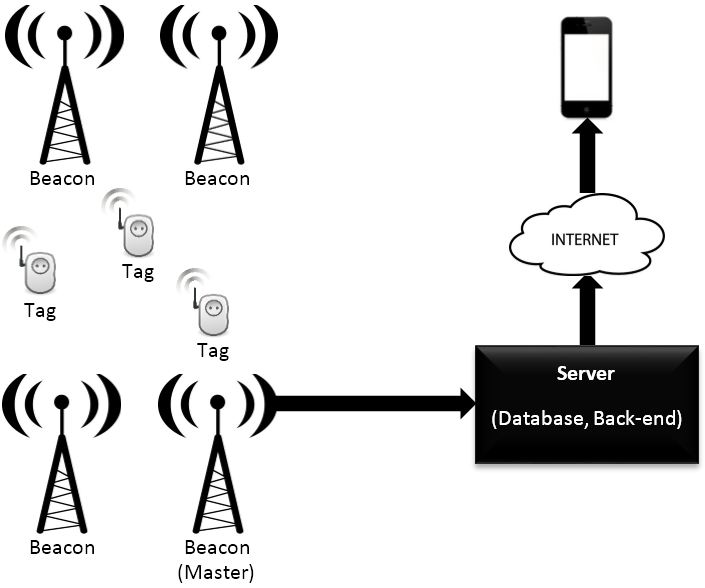
\includegraphics[scale=0.7]{data/software/1.jpg}
\caption{System overview.}
\label{fig:soft-overview}
\end{center}
\end{figure}

\newpage
\subsection{Software Design}
This section will cover aspects relating to the software design of the system. Included is a detailed explanation of how the positions of tags will be determined. A simulation will be used to validate the algorithm and assess how distance error affects the positioning error. The format of the packets that the tags send out will be established, and the back-end database design will be presented.

\subsubsection{Positioning using Trilateration} \label{trilateration}
Trilateration is a geometric process by which the coordinates of a point of interest can be determined by measuring the distance from that point to at least three other known reference points. In the two dimensional case (which we will consider for relatively level parking areas), each distance measurement corresponds to the radius of a circle centred at its respective reference point. The unknown point of interest is located at the intersection point of the three circles.
Figure 6.3.2-1 below illustrates the process. P1, P2 and P3 are known reference points at respective distances r1, r2 and r3 from the point of interest, B. It is clear why a minimum of three reference points are needed. If only one reference point is used, the point of interest could be located anywhere on the circumference of the circle around the point. If two reference points are used (P1 and P2, for example), the resulting circles drawn intersect at a maximum of two places – points A and B in the figure. A third reference point is required to narrow down the possible locations to one.
In the parking system application, the point of interest is a vehicle (specifically, the tag inside the vehicle), and each beacon is a reference point. It should be noted that although only three beacons are required, a fourth beacon is added to the final system for redundancy. 

\begin{figure}[H]
\begin{center}
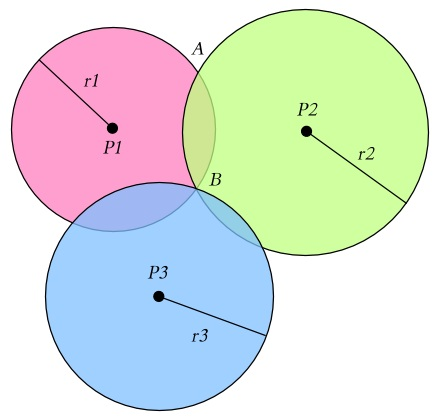
\includegraphics[scale=0.6]{data/software/2.jpg}
\caption{Process of trilateration.\cite{4}}
\label{fig:trilateration}
\end{center}
\end{figure}

The means by which the tag's distance to each beacon is determined will now be explained. It is noteworthy that there are multiple methods to estimate the required distance in this application. A few alternatives will briefly be discussed, and the final selection will be expanded upon.

\newpage
\lsec{Received Signal Strength Technique}
The first method to be discussed is one which uses the received signal strength (RSS) of the signal. Since the energy of the transmitted signal is known, and the energy of the received signal can be determined at the beacons, an estimate of the distance which the signal has travelled can be calculated. However, this requires the assumption of the path loss exponent n. Unfortunately, the value of n can vary, and an exceptionally accurate estimate of its value is needed in order to calculate the distance without any significant level of error. As a result, currently this technique cannot produce a mean accuracy of less than five metres.\cite{gaffney}

\lsec{Time of Flight Technique}
Another technique which can estimate the distance from the tag to the surrounding beacons uses an estimate of the time of flight of the transmitted packet. If the transmission time at the tag and the arrival time at the beacon are known, then the distance between the two can trivially be determined since the propagation speed of the signal is the speed of light. With the assumption that the clocks in the tags and the beacons are synchronized, this method can yield very accurate estimates of the distance. However, crystal effects mean that the clocks will drift with respect to each other over time.\cite{gaffney} This can be combated by periodically sending out clock synchronization packets to the tags, but this is not viable for this application because the tags are to be designed only to periodically transmit and never receive. This is a strict requirement put in place in order to ensure a sufficiently long battery life for the tags. Therefore, this alternative is not suitable.

\lsec{Time Difference of Arrival Technique}
The final technique to be discussed is a modification to the previous method described above. As previously stated, the location of a tag can be determined by finding the intersection of three circles, each centred at a beacon. The radius of each circle is the distance, given by the product of the time of flight of the transmitted signal and the speed of light. The equations of the three circles are as follows\cite{gaffney}:
$$(\tau_1 c)^2 = (x_1-x_t)^2 + (y_1-y_t)^2$$
$$(\tau_2 c)^2 = (x_2-x_t)^2 + (y_2-y_t)^2$$
$$(\tau_3 c)^2 = (x_3-x_t)^2 + (y_3-y_t)^2$$
Where:
\begin{itemize}
\item $\tau_n$ is the time of flight between the tag and the beacon n,
\item $c$ is the speed of light,
\item $(x_n,y_n)$ is the location of beacon n, which is known, and
\item $(x_t,y_t)$ is the location of the tag, which is unknown.
\end{itemize}
Solving the intersection of the above equations will allow the determination of the location of the tag. The problem is that with tags using clocks which are unsynchronized with the beacons, the time of flights $\tau_n$ cannot be determined.

The solution is the time difference of arrival (TDOA) technique. This technique is also known as multilateration. It computes the time difference of arrival of a packet transmitted from the tag to the beacons. Only the beacons are assumed to have synchronized clocks. This technique will now be demonstrated.

\newpage
Assume that at a time $t_0$, a tag transmits a packet. Beacons 1, 2 and 3 each receive the packet at times $t_1$, $t_2$ and $t_3$ respectively. The time of flights are then given by the equations below:
$$\tau_1 = t_1 - t_0$$
$$\tau_2 = t_2 - t_0$$
$$\tau_3 = t_3 - t_0$$
Allow the time difference of arrival (or the difference in the time of flight) between beacon 1 and beacon 2 to be $\Delta \tau_{12}$. By definition, it is given by the following equation:
\begin{equation*}
\begin{split}
\Delta \tau_{12} &= \tau_1 - \tau_2\\
 &= t_1 - t_0 - t_2 + t_0\\
 &= t_1 - t_2\\
\end{split}
\end{equation*}
Taking beacon 3 as the system origin and defining its position as (0, 0), it can be written that:
\begin{equation*}
\begin{split}
\Delta \tau_{13} &= \frac{1}{c} \sqrt{(x_1-x_t)^2 + (y_1-y_t)^2} - \frac{1}{c} \sqrt{(x_3-x_t)^2 + (y_3-y_t)^2}\\ 
&= \frac{1}{c} (\sqrt{(x_1-x_t)^2 + (y_1-y_t)^2} - \sqrt{x_t^2 + y_t^2})
\end{split}
\end{equation*}
\begin{equation*}
\begin{split}
\Delta \tau_{23} &= \frac{1}{c} \sqrt{(x_2-x_t)^2 + (y_2-y_t)^2} - \frac{1}{c} \sqrt{(x_3-x_t)^2 + (y_3-y_t)^2}\\ 
&= \frac{1}{c} (\sqrt{(x_2-x_t)^2 + (y_2-y_t)^2} - \sqrt{x_t^2 + y_t^2})
\end{split}
\end{equation*}
The equations above define two hyperbolae - the intersection of which gives the tag location (xt,yt).\cite{gaffney}

\subsubsection{Simulation}\label{sim}

While the TDOA method described above is mathematically sound, it is somewhat unknown what the positioning accuracy will be in the real world with error caused by signal attenuation and other factors which have been thus far ignored. In order to better visualize the accuracy and effectiveness of the TDOA trilateration technique, a simple simulation was programmed in C\#. Figure~\ref{fig:distance-error} shows a screenshot of the running simulation.

\begin{figure}[H]
\begin{center}
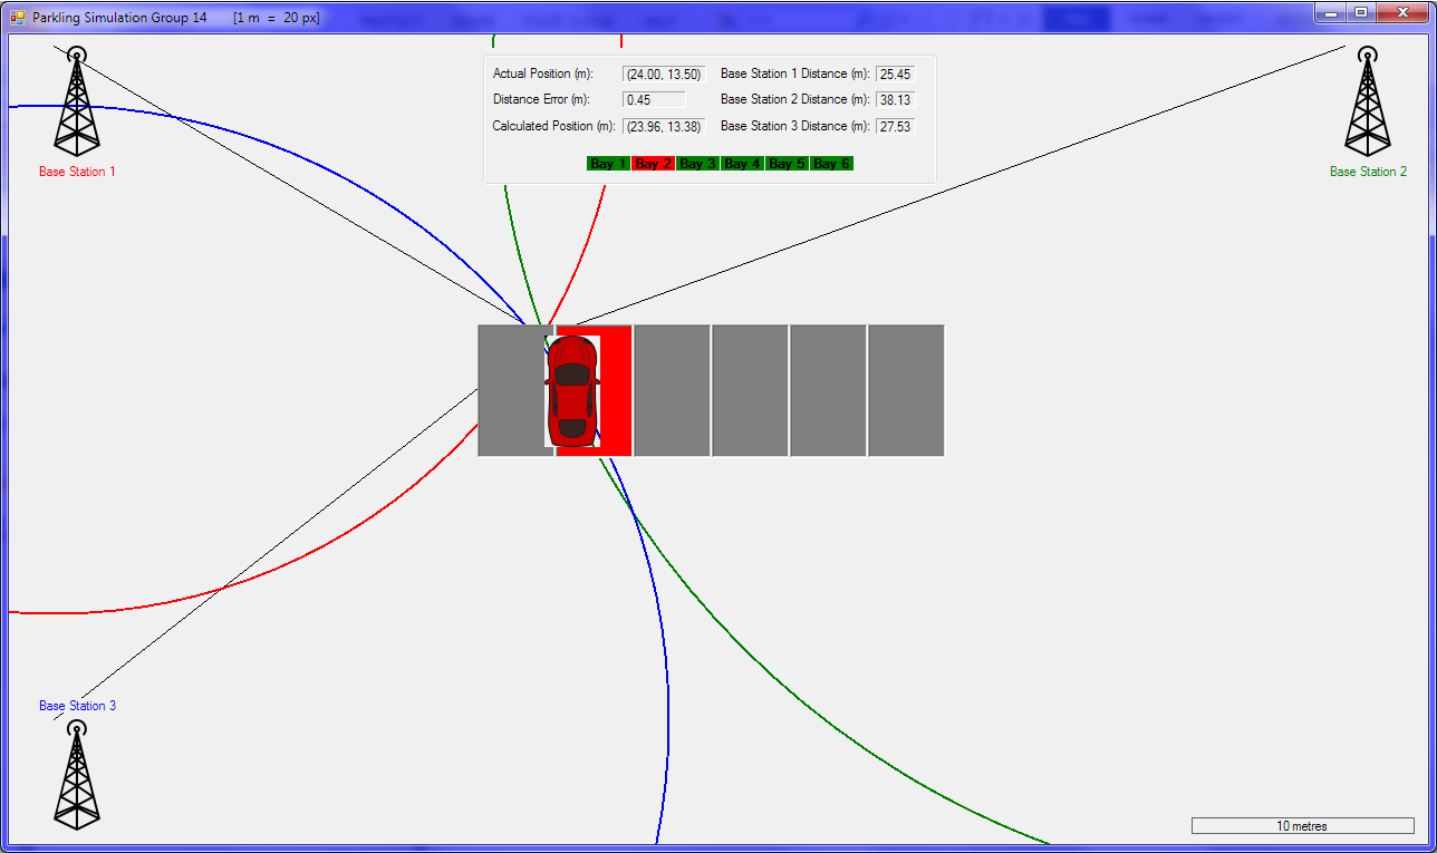
\includegraphics[scale=0.3]{data/software/3.jpg}
\caption{Simulation used to test the effect of distance error on positioning accuracy.}
\label{fig:distance-error}
\end{center}
\end{figure}

\lsec{Simulation Algorithm}
The simulation determines the position of a vehicle and checks whether it is in a parking bay according to the following, simplified algorithm:

\begin{enumerate}
\item The exact distance from the vehicle to each of the beacons is determined geometrically.
\item A random error with adjustable maximum scale (in the range from 0 - 1 m) is introduced into each of the three distance measurements.
\item The two intersection points of the circles centred at beacons 1 and 2 are determined.
\item The intersection point closest to beacon 3 is taken as the location of the vehicle.
\item The simulation checks whether the calculated location is in the region of any of the parking bays.
\end{enumerate}

\lsec{Sources of Error}
Clock drift introduces an insignificant error in the TDOA trilateration technique (as long as the beacons are synchronized often enough). Another source of error comes from the fact that, effectively, the reported distance varies slightly (as figure~\ref{fig:reported-distance} shows) according to the received signal level. This error could be sufficiently large to become problematic for the parking system application. However, it can be compensated for using Friis' well-known path loss formula.\cite{2}

\begin{figure}[H]
\begin{center}
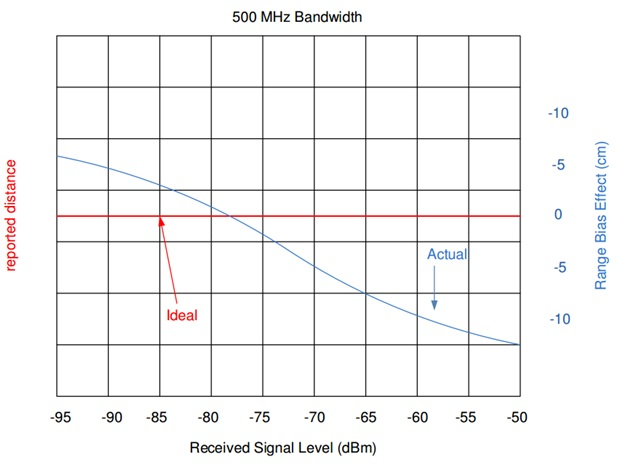
\includegraphics[scale=0.8]{data/software/4.jpg}
\caption{The effect of received signal level on the reported distance.\cite{2}}
\label{fig:reported-distance}
\end{center}
\end{figure}

\newpage
The only remaining potentially significant source of error is that caused by signal attenuation resulting from the tag's transmission having to pass through at least one vehicle body and potentially other obstacles. This can be minimised by ensuring that the beacons are high enough above ground level (to minimize the number of vehicle bodies that the signal must propagate through) and maintaining the surrounding area (by trimming foliage and clearing other obstacles). Regardless, some error will be introduced into the system, and the simulation was used to determine the effect of distance error.

\lsec{Findings of the Simulation}
The simulation revealed that the system was surprisingly tolerant to errors in distance. Using a distance error with a maximum magnitude below 0.50 m, even a car parked partially (about 15\%) in another bay was detected correctly 100\% of the time. Since the error introduced by variation in the received signal level can be nearly eradicated using Friis' path loss formula, it is concluded that the system will be accurate enough, with the assumption that the distance error will be less than 0.50 m. This appears to be a very safe assumption as the DecaWave chips are quoted as giving a positioning accuracy up to 0.10 m indoors.\cite{3}

\subsubsection{Tag Packet Format} \label{tag-packet}
This subsection will briefly outline and justify the contents of the packets that tags will emit. Each data packet will have the following data:

\begin{itemize}
\item The ID of the tag – to identify the tag and therefore vehicle and user.
\item Time the packet was transmitted – to be used in the TDOA calculation.
\item Battery level of the tag – to inform the user via the app/email/SMS that the battery is low.
\end{itemize}

These packets will be periodically transmitted by each tag every 5-10 minutes in order to conserve their battery life.

\subsubsection{Database Design}
This subsection will detail the design of the parking system database. Specifically, the design of each of the three main tables required to make the system work is presented and explained. The three main tables are:

\begin{itemize}
\item Parking Areas
\item Parking Bays
\item Tags
\end{itemize}

The design of these tables will be expanded upon below:

\newpage
\lsec{Parking Areas}

\begin{table}[H]
\begin{center}
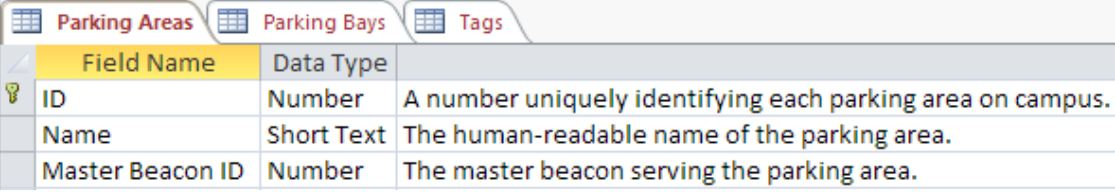
\includegraphics[scale=0.5]{data/software/5.jpg}
\caption{Parking Areas table.}
\label{tbl:table-parking-areas}
\end{center}
\end{table}

Table~\ref{tbl:table-parking-areas} shows the design of the Parking Areas table. This is a simple table in which each parking area has a record. The purpose of the Master Beacon ID field is so that the server knows which parking area the information it receives relates to, based on which master beacon it received the information from.

\lsec{Parking Bays}

\begin{table}[H]
\begin{center}
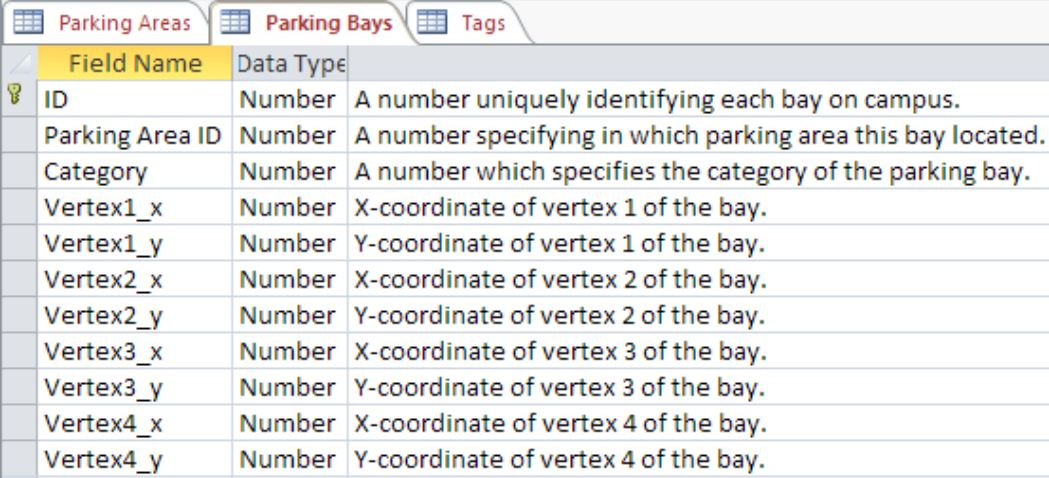
\includegraphics[scale=0.5]{data/software/6.jpg}
\caption{Parking Bays table.}
\label{tbl:table-parking-bays}
\end{center}
\end{table}

Table~\ref{tbl:table-parking-bays} shows the design of the Parking Bays table. Every single parking bay on campus will be entered as a record in this table. The Parking Area ID field details in which parking area each bay is located. The category field can be updated via the traffic department's client app as required. For example, student bays could be reassigned to be postgraduate bays. The eight vertex fields define the coordinates of each of the four corners of the parking bay. This is used to determine which bay a tag is occupying, if any.

\newpage
\lsec{Tags}
\begin{table}[H]
\begin{center}
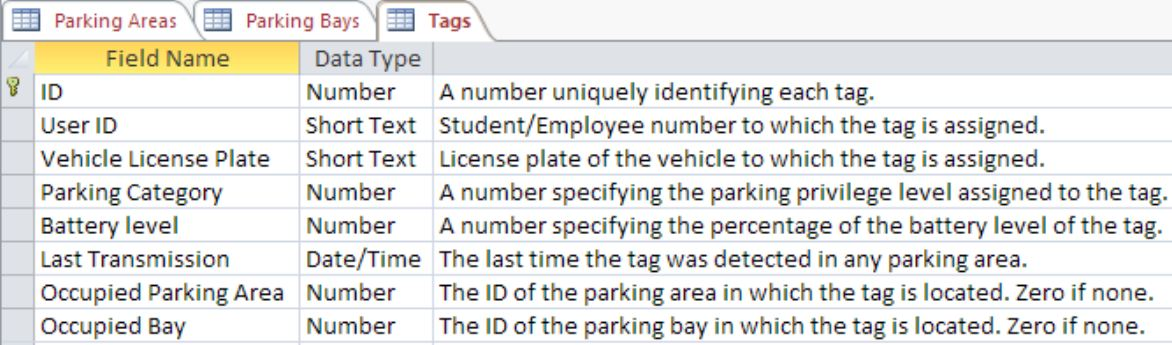
\includegraphics[scale=0.37]{data/software/7.jpg}
\caption{Tags table.}
\label{tbl:table-tags}
\end{center}
\end{table}
Table~\ref{tbl:table-tags} shows the design of the Tags table. The design of this table takes into consideration that a single user may have multiple vehicles and therefore multiple assigned tags, but the tag-vehicle relationship is one-to-one. This means that each tag can only be assigned to one vehicle, and a vehicle can only have one tag assigned to it.

The parking category field is used to determine whether the user is allowed to park a specific tag/vehicle in any given bay. The tag's reported battery level is stored in order to notify the user via the mobile app/email/SMS that the battery is low and needs to be replaced.
The Last Transmission field is used for statistics to keep track of how long users spend on campus.

\subsubsection{Mobile and Web Application}
This subsection will briefly outline the functionality of the mobile and web application. The two applications will have the same features. Each user logs in with their student/employee number and UCT password. There will be only one type of app, regardless of the user type. There will be three user types:

\lsec{Admin Users}
These users are able to control the assignment of parking bay categories. They also have access to statistical information that can be used to monitor patterns on campus in order to improve the parking system.

\lsec{Traffic Officials}
These users have the ability to view the location of illegally parked cars and mark them once they have been fined or clamped.

\lsec{Parking Users}
These users receive information about parking availability (via their smartphone's screen, or a synthesized voice to allow operation while driving) according to their assigned parking category and preferred parking areas. They will also be given an estimated time (determined from historical data) by which they must arrive on campus if they wish to park in their preferred parking area.

The parking users will be informed if they have parked illegally, been fined or clamped. They will be able to view the last location and battery status of each of their vehicles/tags, provided the tags are located in a parking area on campus.

\newpage
\subsection{Mechanical Design} 
This section details the mechanical components design of the transceiver chips.

\subsubsection{Tag Case}
\begin{figure}[H]
\begin{center}
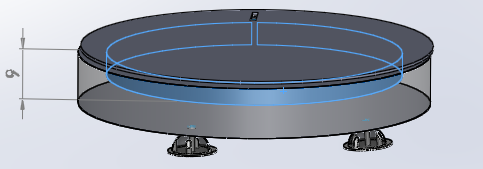
\includegraphics[scale=0.6]{data/mechanical/1.png}
\caption{Tag case (thickness 9 mm).}
\label{fig:mech-1}
\end{center}
\end{figure}

\begin{figure}[H]
\begin{center}
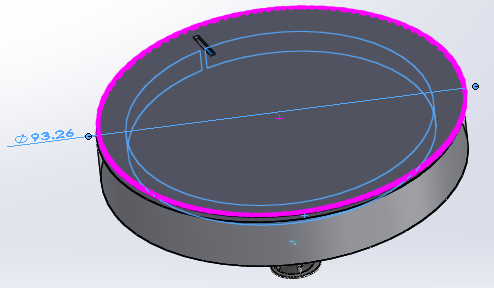
\includegraphics[scale=0.6]{data/mechanical/2.png}
\caption{Tag case (diameter 93.26 mm).}
\label{fig:mech-2}
\end{center}
\end{figure}

Designed to enclose the Printed Circuit Board (PCB) circuitries for the transceiver chips. Figures~\ref{fig:mech-1} and \ref{fig:mech-2} shows the dimensions of the case.

\lsec{Material}
The structural case is made from acrylic (thermoset plastic), which cannot change shape by reheating. The material is cheaper and lightweight than its counterparts such as Bakelite and Melamine.\cite{fig:mech-1} It is capable of withstanding weather and is stable in sunlight. The case will be mounted atop the dashboard of the car, in order for it to be visible and its material shape preserved.

\newpage
\lsec{Mounting}
\begin{figure}[H]
\begin{center}
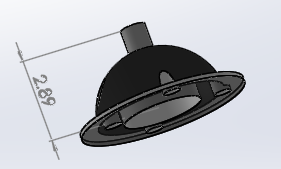
\includegraphics[scale=0.6]{data/mechanical/3.png}
\caption{Suction-cup (height 2.89 mm).}
\label{fig:mech-3}
\end{center}
\end{figure}

\begin{figure}[H]
\begin{center}
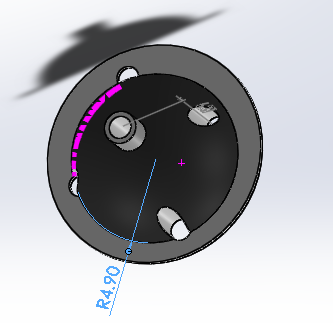
\includegraphics[scale=0.5]{data/mechanical/4.png}
\caption{Sucker radius 4.9 mm of suction.}
\label{fig:mech-4}
\end{center}
\end{figure}

The case will be mounted using suction-cups (shown in figure~\ref{fig:mech-3}), made from rubber, and attached to its base. The suckers use the negative fluid pressure of air to create a partial vacuum and adhere to the dashboard.\ref{fig:mech-2} The chosen diameter (as shown in figure~\ref{fig:mech-4}) is 9.8 mm, and will provide the necessary resistive detachment force. The minimum force required to detach is given by the following equation:
$$F=PA$$
The pressure outside one suction-cup, P, will typically be 1 atmosphere, thus the force required to lift the base from dashboard (at the point of one suction-cup) is about 31 Newtons.\ref{fig:mech-2}

\lsec{Identification}
\begin{figure}[H]
\begin{center}
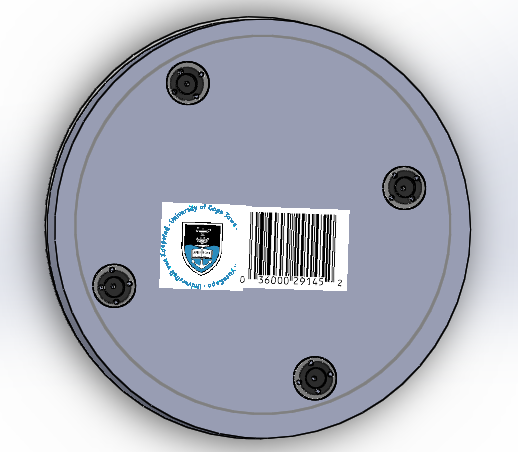
\includegraphics[scale=0.4]{data/mechanical/5.png}
\caption{Tag case base with bar-code.}
\label{fig:mech-5}
\end{center}
\end{figure}

The case will have a bar coded sticker as shown in figure~\ref{fig:mech-5}. This will ensure the chip is identifiable. It will also be used in sanction drivers who are prohibited to park at a specific parking bay or simply incorrectly parked.

\lsec{Evaluation}
SolidWorks Software Design Evaluation was made to the casing structure, and the following are the estimate calculations of the component:

\begin{center}
Total Mass = 82 g \\
Volume = 102985 $mm^3$
\end{center}

(Drawing designs refer to appendix G2.)

\lsec{Direct Costs}
3 mm acrylic: starts at R73.61/sq.ft \\
Laser cutting costs: starts at R2.21/inch \\
4.1 mm rubber: starts at R51.52/sq.ft 

Cost of manufacturing in South Africa per tag case is estimated to cost R180.00.

\subsubsection{Beacon Structure}

The structure of the beacon is shown in figure~\ref{fig:mech-6}. It is constructed from mild steel which is immensely strong. The material also has a strength of bending without cracking in adverse environmental conditions, this offers the advantage especially when subjected to a greater forces.\ref{fig:mech-3}

\begin{figure}[H]
\begin{center}
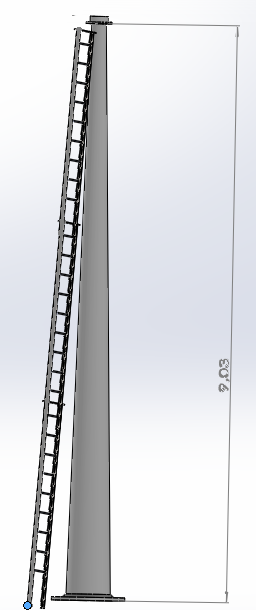
\includegraphics[scale=0.4]{data/mechanical/6.png}
\caption{Beacon design.}
\label{fig:mech-6}
\end{center}
\end{figure}

\begin{figure}[H]
\begin{center}
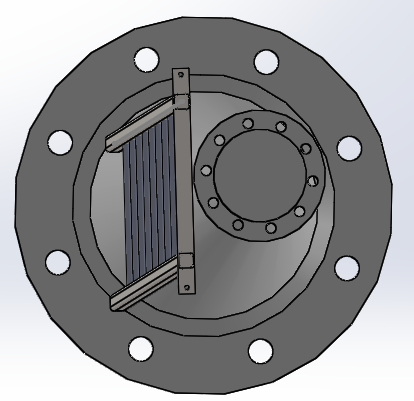
\includegraphics[scale=0.3]{data/mechanical/7.png}
\caption{Top view of the beacon.}
\label{fig:mech-7}
\end{center}
\end{figure}

Mild steel is often chosen because of its strength, low weight and speed of construction.\ref{fig:mech-4}

\lsec{Evaluation}
SolidWorks Software Design Evaluation was made to the beacon, and the following are the estimate calculations of the component:
\begin{center}
Total mass = 1754 [$kg$]\\
Volume = 1.7 [$m^3$]\\
Centre of mass(x,y,z) = (0.01, 5.82, 0.01) [$m$]\\
Moments of inertia taken at the centre of mass aligned with the coordinate systems.\\
Lxy = 1.47 [$kg.m^2$]\\
Lyz = -44.54 [$kg.m^2$]\\
Lzz = 10523.05 [$kg.m^2$]
\end{center}

The dynamics make the structure durable and capable of withstanding the forces that may lead to deformation and toppling torques.

(Drawing designs refer to appendix G1.)

\lsec{Direct Costs}
3-80mm thickness mild steel: starts at R7378.17/ton\\
Each beacon is estimated to cost R12 000.00

\subsubsection{Beacon Placement}
Figure~\ref{fig:mech-8} in Appendix H  shows the location of parking areas on UCT Upper Campus and figure~\ref{fig:mech-9} in Appendix H shows where the beacons will be placed in relation to these parking areas - with 4 beacons within a 150m range of each parking area including one master beacon per parking area.

\newpage
\subsection{Electrical Design} 
\subsubsection{Power Requirements}
\lsec{Overview}
In order to power the beacons, certain specialised circuitry is required. These are known as voltage regulators. They are necessary for two different reasons in our design namely:

\begin{itemize}
\item The first voltage regulator is used for the solar powered beacons. Solar power generated is unstable and can damage electrical components if it is not regulated using a VC.
\item The second voltage regulator is powered via the mains. The AC voltage that comes from the mains is not suitable for use in the circuits. It first needs to be stepped down and then converted into DC.
\end{itemize}

Two voltage regulators were designed; one for the mains and one for the solar panels.

\lsec{Power Budget for Beacon}
Using datasheet values for the three ICs the following rough power budget was constructed:

\begin{figure}[H]
\begin{center}
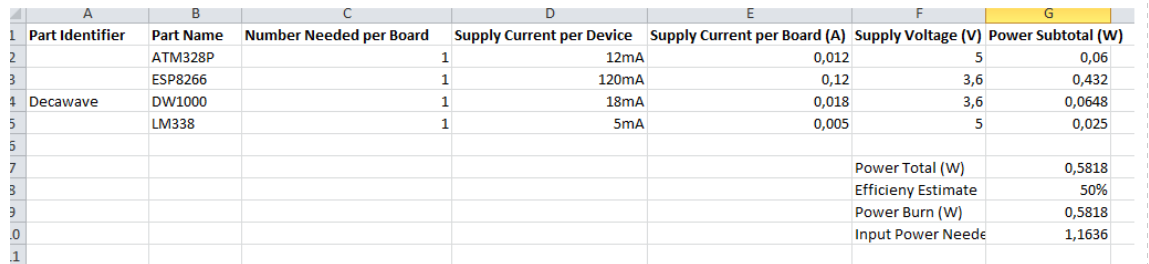
\includegraphics[scale=0.4]{data/power/1.png}
\caption{Power.}
\label{fig:pow-1}
\end{center}
\end{figure}

This table assumes that 50\% of the power used will be dissipated. This was done for design
purposes. It can be seen that the beacon requires a fairly low estimate of power (roughly 1.2W) and
so some cost saving measures in the design can be taken. These will be specified.

\lsec{Power Supply Design}
\textit{Design requirements - Regulators:}

We need to design voltage regulators which regulate the voltage to levels appropriate for the ICs
used in our design namely the ATM328P and ESP8266 as well as the Decawave DW1000.
From the datasheets the required value ranges for both are summarised as:

Input Voltage: 1.8V-5.5V, Output Voltage 2.1V – 4.2V, Current Rating 40mA

The primary goal of our voltage regulators will be to get around 5V outputted to the circuit.
We also want the regulators to be power efficient and have low dissipation because of the inherent
inefficiency of solar panels. In addition the regulators need to be as robust and as cheap as possible.

\textit{Design requirements - Solar Panel:}

The solar panel needs to be able to provide roughly 1.2W according to the energy budget of power
for the circuitry to work. This is a small amount. The solar panel will be assumed to have an
efficiency of 20\%. There are roughly 12 hours of sunlight in a day, so the assumption will be that our
solar panels will only be exposed to light for 5 hours every day, assuming the most overcast possible
winter's day. The actual amount will be much higher, but the design assumes the worst case.

This equates to 1.282 Wh a day.

The solar panel traps solar energy and produces an output voltage. But, since the light radiation
falling on the solar panel can vary, the output voltage becomes unstable. For our purposes, stable
voltage is required. So, to make the output voltage stable and regulated, we use a voltage regulator
circuit along with the solar panel.

With these considerations the following solar panel was selected:

Sirius Solar Energy Systems SS-005-12, 5W 12V rating. The model size is 253 x 279 x 22mm

\lsec{Solar Panel Voltage Regulator}
\textit{Selecting a voltage Regulator:}

The LM 7805 Voltage Regulator was selected because it can regulate a steady output voltage of 5V
which is what we need for our ICs. It is also easy to use and relatively cheap.

\textit{Battery Selection:}

We require rechargeable batteries. Four LiPO batteries were selected for this purpose. They are
relatively cheap rechargeable batteries and have a sufficient lifespan. Even though their cost seems
prohibitive, they will actually greatly extend the functionality of the system, in addition to saving
large amounts of money on electricity tariffs. 3 were selected in order to get the voltage to 4.8V.

\textit{Simulations:}

\begin{figure}[H]
\begin{center}
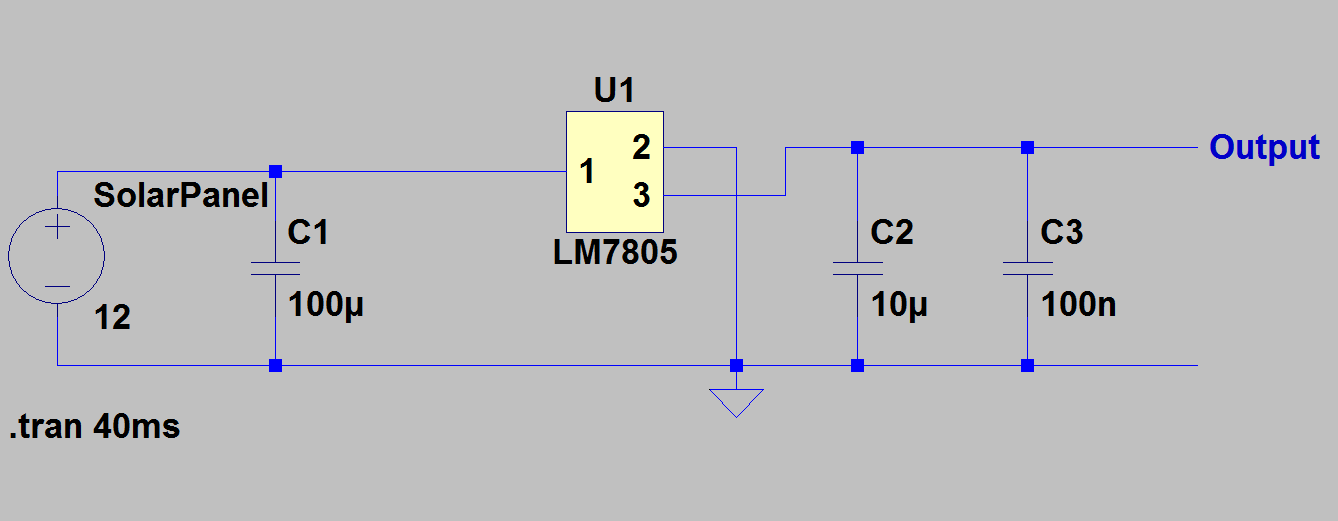
\includegraphics[scale=0.4]{data/power/2.png}
\caption{Initial regulator using datasheet example.}
\label{fig:pow-2}
\end{center}
\end{figure}

\begin{figure}[H]
\begin{center}
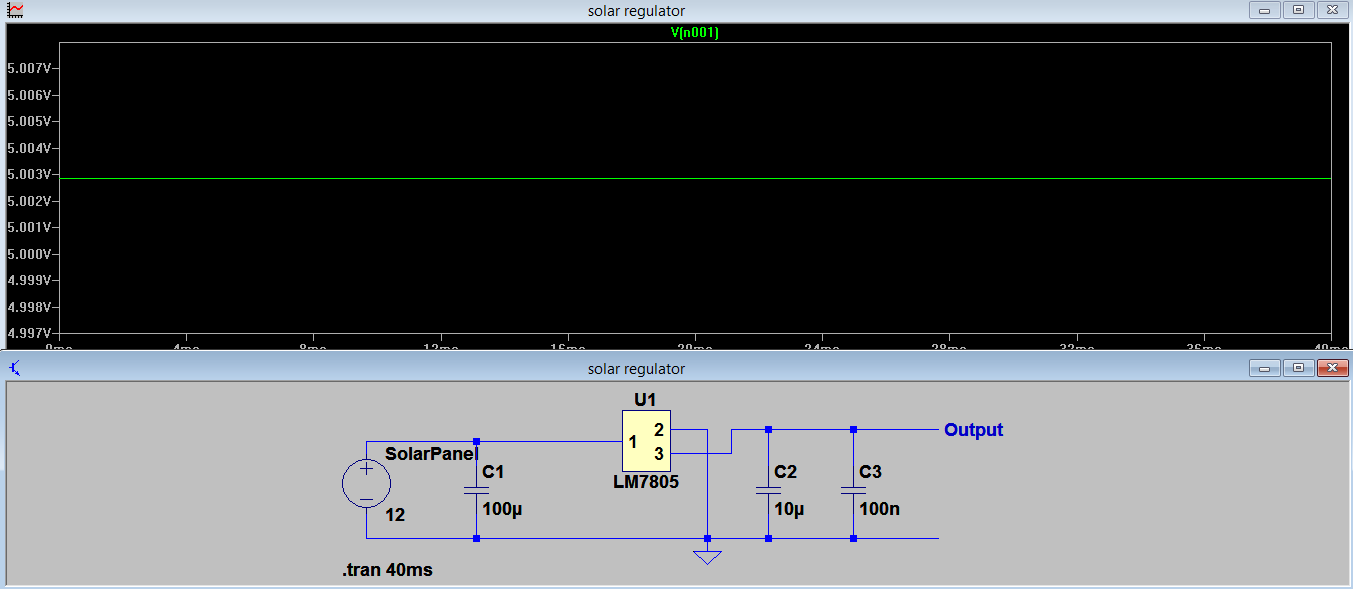
\includegraphics[scale=0.3]{data/power/3.png}
\caption{Voltmeter reading for initial circuit showing 5.003V.}
\label{fig:pow-3}
\end{center}
\end{figure}

The initial circuit was set up and tested in LTspice.

As can be seen from the Ltspice simulation, the output voltage is regulated to 5.03V which is roughly
what we need for the beacon circuitry.

The most obvious improvement would be to use a battery to store excess power generated. This is
doubly important for solar panels as they can be unreliable. To keep the device running, a battery
can be attached in parallel as a backup power source. Diodes are connected to the battery and the
solar panel. This is a failsafe in case the battery is installed backwards accidentally as the diodes will
prevent the battery from receiving power from the solar panel since it is a one-way valve.

When the solar panel receives enough light, the device runs entirely from the solar panel. Our design
aim is for the battery to have a lower voltage rating than the outputted rating from the voltage
regulator. Current only flows from a higher voltage to a lower voltage, so when there is sufficient
power from the solar panel, the battery won't be used at all.

When the solar panel and the battery pack are at the same voltage, they will both contribute to
running the device. This will extend the life of a device with an otherwise underpowered solar panel.

Finally, when the solar panel isn't receiving enough light, its voltage will drop below that of the
battery – and the battery will now power the circuit.

Diodes are very cheap and their inclusion is a far superior option to replacing a device due to a
potential reversed-battery error.

The final design for the regulator is show below:

\begin{figure}[H]
\begin{center}
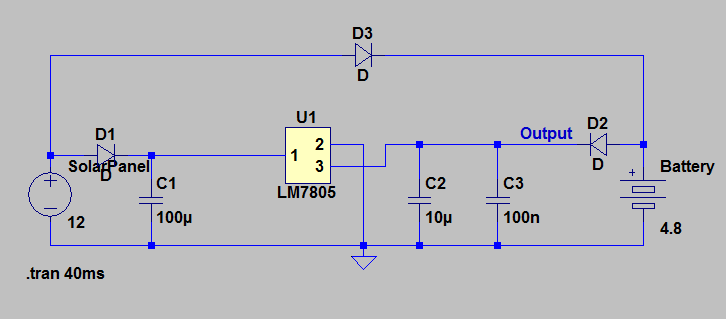
\includegraphics[scale=0.4]{data/power/4.png}
\caption{Regulator final design.}
\label{fig:pow-4}
\end{center}
\end{figure}

\begin{figure}[H]
\begin{center}
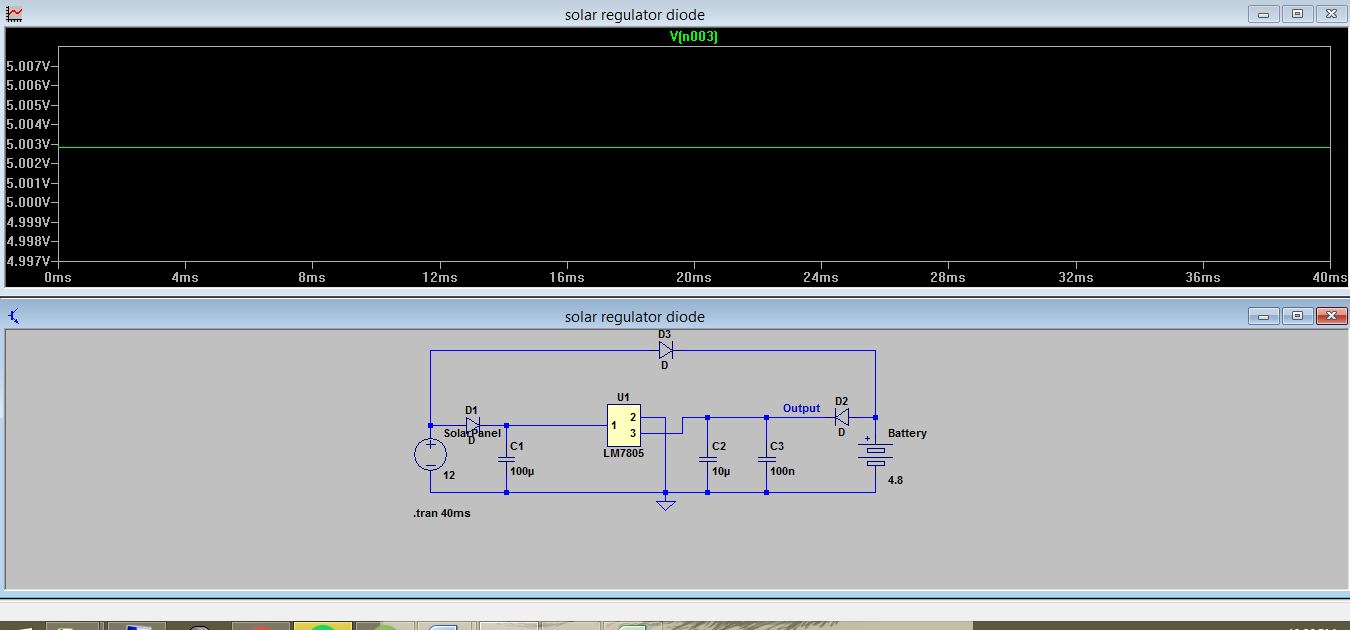
\includegraphics[scale=0.3]{data/power/5.png}
\caption{Regulator final design simulation.}
\label{fig:pow-5}
\end{center}
\end{figure}

As can be seen the output voltage is roughly 5V which satisfies our requirements. The additional
components – the battery and the diodes – provide additional functionality and protection. NOTE:
The location labelled output on the circuit is where the beacon circuitry will be installed.

\textit{Bill of Materials for Solar Regulator:}

\begin{figure}[H]
\begin{center}
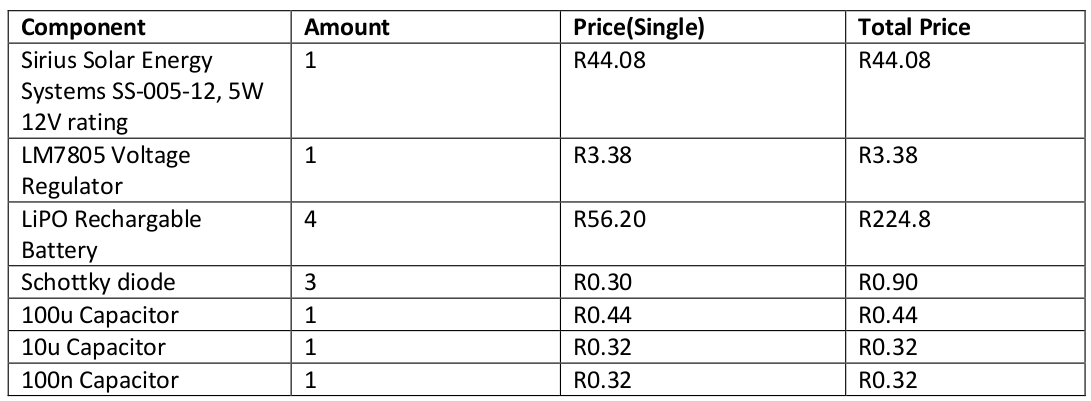
\includegraphics[scale=0.3]{data/power/tb1.png}
\caption{BOM for Solar Regulator.}
\label{fig:pow-BOM}
\end{center}
\end{figure}

\lsec{Mains Voltage Regulator}
This voltage regulator will differ from the one required for solar panels. In South Africa our mains are
rated at 230V 50Hz so the design will revolve around this. The mains AC voltage needs to be
converted to a usable DC voltage.

To achieve this we need to design a voltage regulator taking note of 4 main components:

\begin{enumerate}
\item A Step Down Transformer (to step down the mains)
\item Voltage Regulator
\item Capacitor
\item Diodes
\end{enumerate}

We need 5V so again as specified by the datasheets so I will use the LM7805 voltage regulator which
was previously used in the solar panel regulator. This will also assist in lowering the cost as these
regulators can be bought in bulk.

\textit{Step 1: Transformer Design}

A suitable transformer needs to be selected first. This decision will be based on current rating and
the secondary voltage.

\begin{itemize}
\item For design purposes, the input voltage to the LM7805 (what comes out of the secondary
winding) should be at least 2V greater than the required output. For our purposes this
should be around 7V.
\item The current rating is dependent on the load.
\end{itemize}

Based on these observations we can select a transformer. It was found that a 6-0-6 transformer with
a current rating of 500mA was suitable for design.

\textit{Step 2: Rectifier Design}

The design choice was taken to use a full wave rectifier. It was chosen for the following reasons:

\begin{itemize}
\item It will allow a higher transformer utilization factor. TUC is the ratio of DC power available at
the load resistor and the AC rating of the secondary coil.
\item 1N4148 diodes are used as they can withstand a higher reverse voltage than 1N5818.
\item Less DC saturation
\end{itemize}

\textit{Step 3: Capacitor Choice}
Ripple factor is used to decide which capacitors to use.
$$Y=\frac{1}{4 \sqrt{3fRC}}$$
Where:
\begin{itemize}
\item $f$ = frequency of AC which is 50Hz in South Africa
\item R is calculated via $\frac{V}{I}=\frac{6\sqrt{2}[V]}{500mA}=16.97\Omega$
\item C is the filtering capacitance. This is calculated via:\\
$Y=\frac{V_{AC}-rms}{V_{DC}}$\\
$V_{AC}-rms=\frac{V_r}{2\sqrt{3}}$\\
$V_{DC}=V_{MAX}-\frac{V_r}{2}$\\
$V_r=V_{MAX}-V_{MIN}$\\
The following values are obtained:\\
$V_r=0.4V$\\
$V_{AC}-rms=0.346V$\\
$V_{DC}=5V$\\
$Y=0.06928$\\
With this value of Y we can use the ripple effect equation at the beginning to solve for C
which comes to C = 2314 uF. A 2200uF capacitor is therefore selected for use in the circuit.
\end{itemize}

Additionally the LM7805 datasheet suggests using a 0.01uF capacitor at the output in order to
protect against transient changes in voltage caused by changes in load. The datasheet also suggest
using a 0.33uF capacitor at the input side of the regulator to avoid ripples. Both of these were
factored into the design.

The final circuit designed is shown below. However the transformer was neglected from the final
circuit for simplicity even though it will be used:
\begin{figure}[H]
\begin{center}
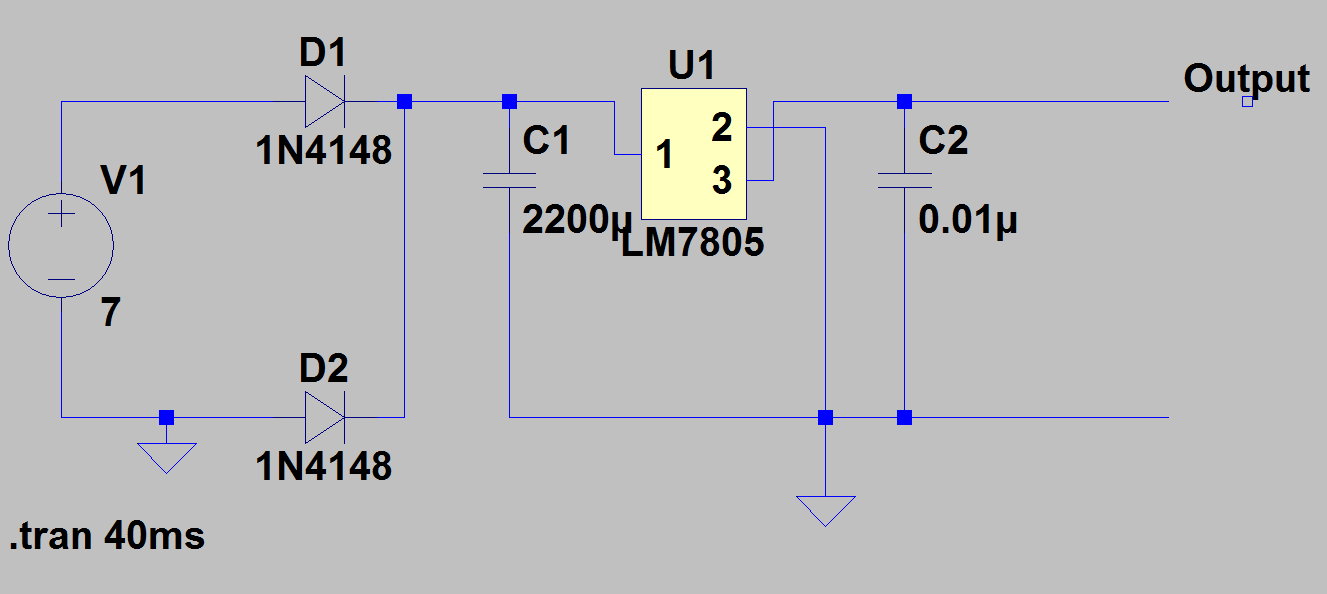
\includegraphics[scale=0.3]{data/power/7.png}
\caption{Final circuit.}
\label{fig:pow-7}
\end{center}
\end{figure}
Checking the output voltage via simulation the following value was obtained:
\begin{figure}[H]
\begin{center}
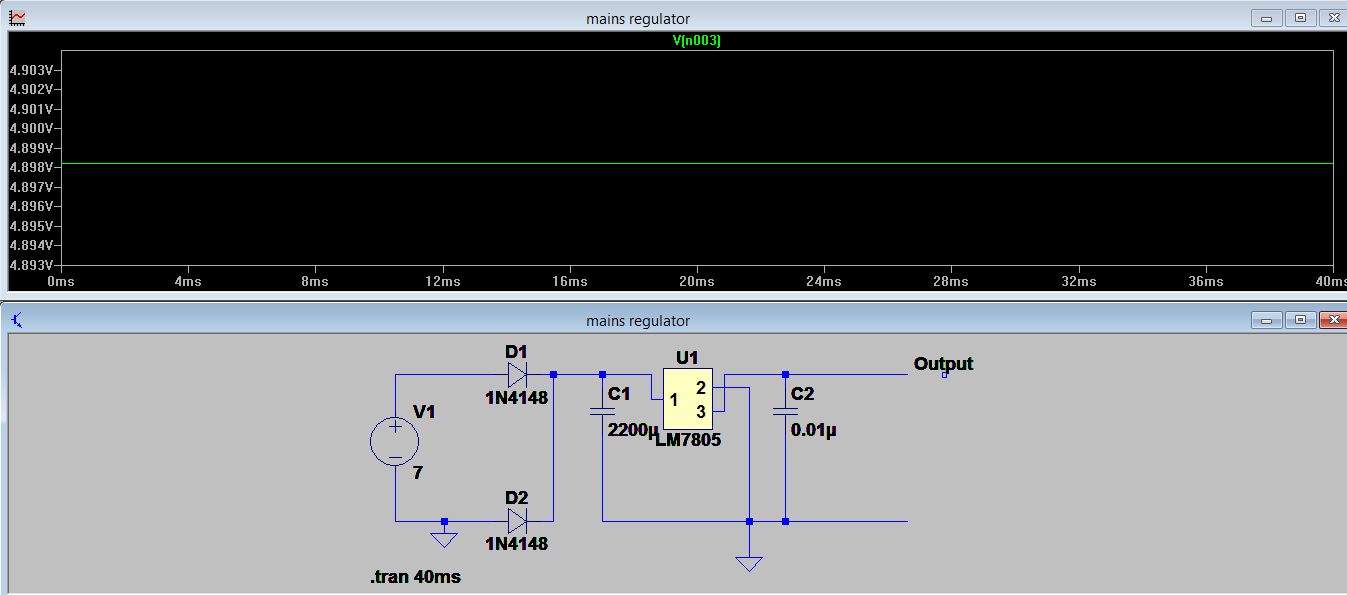
\includegraphics[scale=0.3]{data/power/8.png}
\caption{Final circuit simulation.}
\label{fig:pow-8}
\end{center}
\end{figure}
This value of 4.89V is suitable for use in the beacon.

\newpage
\textit{Bill of Materials for Mains Regulator:}

\begin{figure}[H]
\begin{center}
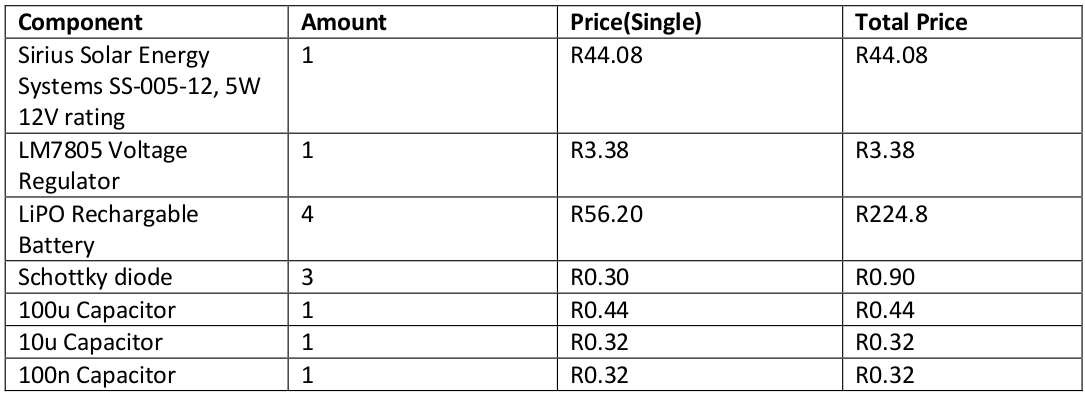
\includegraphics[scale=0.3]{data/power/tb2.png}
\caption{BOM for Mains Regulator.}
\label{fig:pow-BOM2}
\end{center}
\end{figure}

\subsubsection{Schematics (Tag and Beacon)}

The following diagrams cover the design of the tag; where the beacon makes a few changes to the circuitry and adds a WiFi module, seen in Figure~\ref{fig:wifi}. The full schematics can be seen in Appendix C.

The system is made up of three components; namely the \textbf{basic DW1000} schematic sheet, the \textbf{microcontroller} schematic sheet and the \textbf{WiFi} schematic sheet - as seen in Figure~\ref{fig:interface-conn}. The system was designed to be modular so that each section has a set function - the \textbf{basic DW1000} circuit is involved in both the beacons and tags with RF functionality, the \textbf{microcontroller} circuitry is a replaceable section that both the tag and beacon rely on, the \textbf{WiFi} module is only required on the master beacon and is thus also a separate section which together form the system.

\begin{figure}[H]
\begin{center}
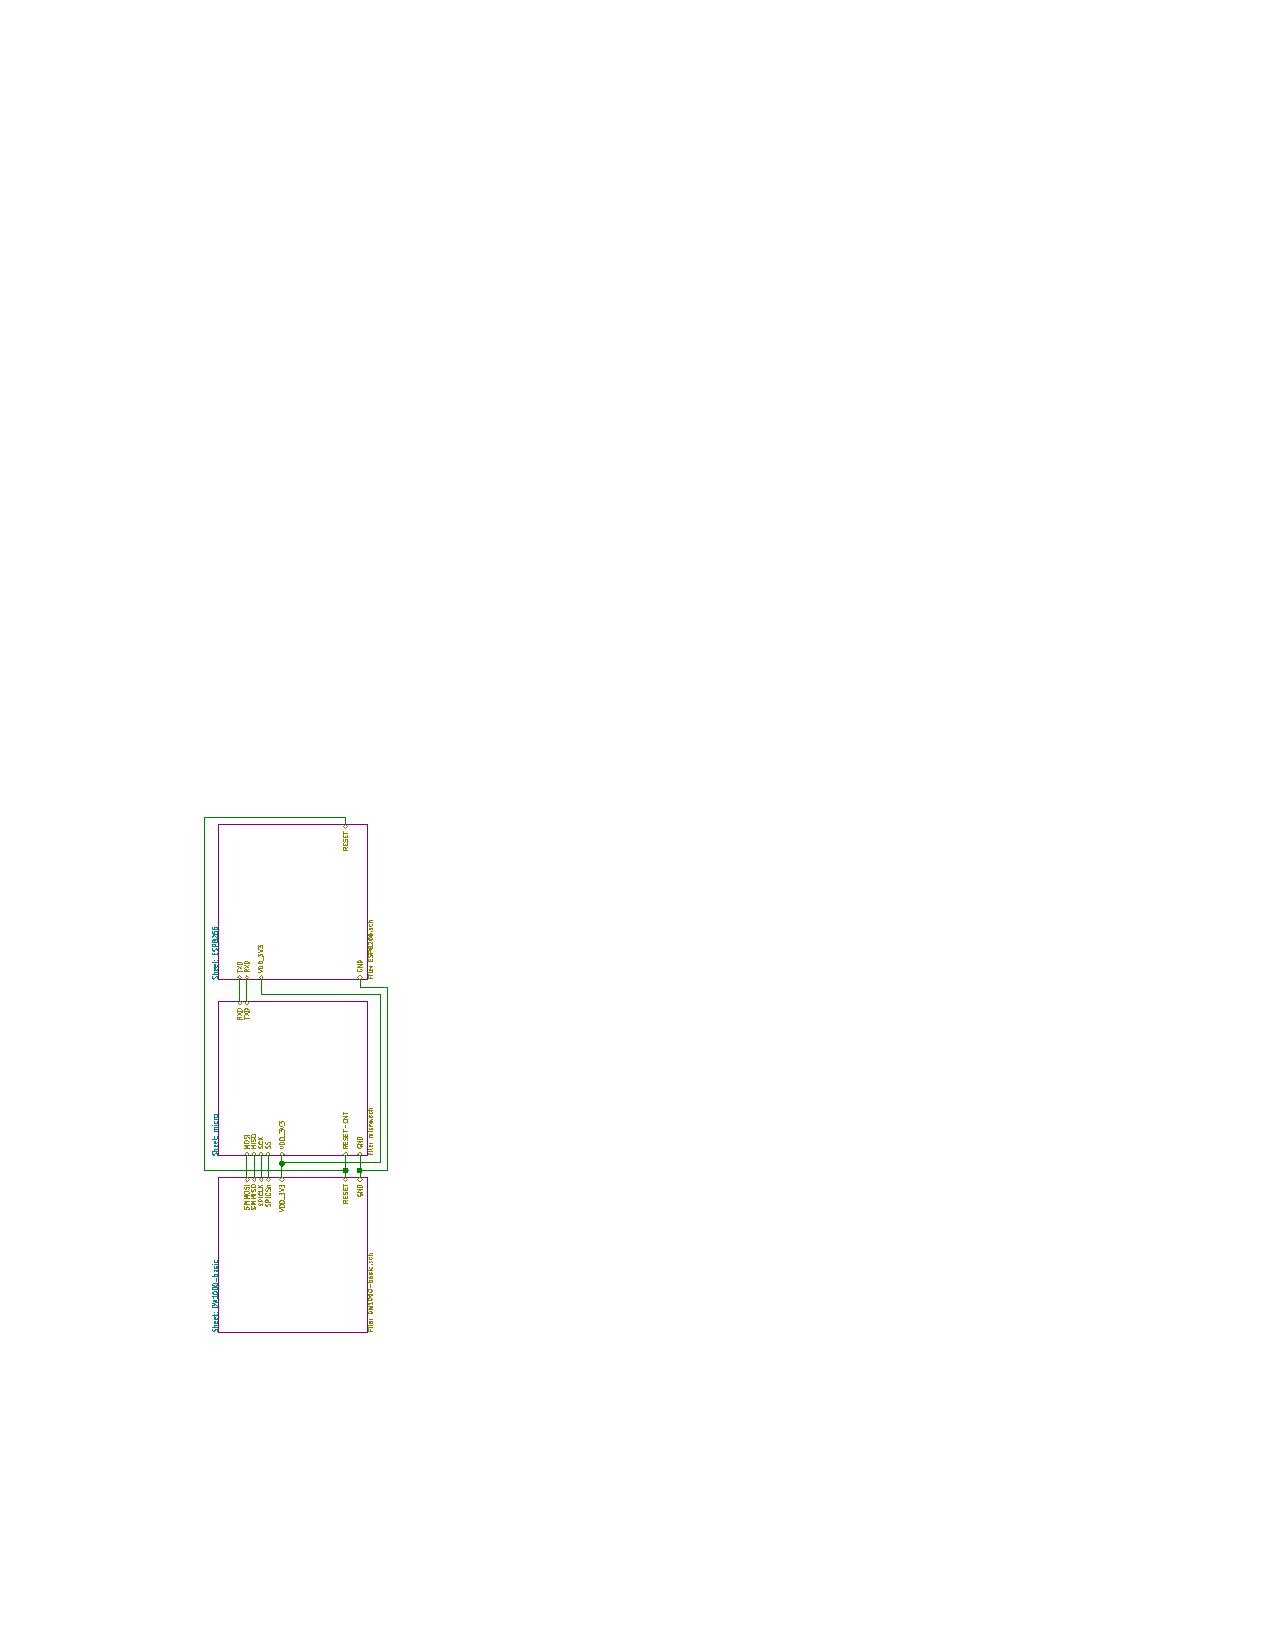
\includegraphics[page=1,scale=1.5,trim={3cm 5cm 15cm 13cm},clip,angle=-90]{data/parking-system2.pdf}
\caption{Parking system tag schematic diagram: interface connections.}
\label{fig:interface-conn}
\end{center}
\end{figure}

\newpage
\lsec{Component Selection}
The Atmel ATmega328P micro controller was chosen for it's low power consumption with five software selectable power saving modes and it's wide 1.8-5.5 V operating range.\cite{atmel} There is also lots of open-source software available for the Decawave on the Atmel chipset, ensuring less programming issues come up. The processing power of the beacon will be shared with the ESP8266 module which has a capable microprocessor on board. The tags are not required to do very much processing on board, so the Atmel chip is suitable for the job.

The ESP8266 WiFi module was chosen for the beacon circuitry because it is well documented and cheaply available while being a reliable and tested system.

Two DC-DC buck converters were used, namely the TPS62203DBVR from Texas Instruments, because of their low supply current of 15uA and high operating efficiency - which will be needed for the tags especially.

In the BOM and costing of Appendix F, components were chosen to optimize costs rather than quality, except where the RF circuitry was involved.

\begin{figure}[H]
\begin{center}
\includegraphics[page=2,scale=0.5,trim={0cm 0cm 0cm 0cm},clip]{data/parking-system.pdf}
\caption{Parking system tag schematic diagram: transceiver chip.\cite{DW-data}}
\end{center}
\end{figure}

\begin{figure}[H]
\begin{center}
\includegraphics[page=3,scale=0.9,trim={10cm 8cm 10cm 5cm},clip]{data/parking-system.pdf}
\caption{Parking system tag schematic diagram: micro-controller.}
\end{center}
\end{figure}

\begin{figure}[H]
\begin{center}
\includegraphics[page=4,scale=1,trim={5cm 9cm 10cm 13cm},clip,angle=-90]{data/parking-system2.pdf}
\caption{Parking system beacon schematic diagram: WiFi module.}
\label{fig:wifi}
\end{center}
\end{figure}

\subsubsection{PCB Design (Tag and Beacon)}
The PCB design for the tag and beacon can be seen in Appendix D and E respectively. The PCBs were designed and routed using the open source software KiCad, to reduce design costs. Decoupling capacitors were placed as close as possible to their relevant power terminals. Traces were optimized to be as short as possible and to reduce ground feedback loops which could pick up RF interference. The traces for the antenna were placed as close as possible to the antenna terminal and in the case of the tag a chip antenna was used. 

EMF and RF mitigation techniques have to be considered when designing the PCBs in order to make them compliant with the ICASA regulations. This involved using a ground plane and ensuring the antennas are correctly matched ($100\Omega$ traces) to reduce RF harmonic signals.

\subsubsection{RF Design}
\lsec{Antenna Specifications:\cite{DW-antenna}}

Friis' Transmission Equation states the following:
$$P_{RX} = \frac{P_{TX}G_{TX}G_{RX} \lambda^2}{(4 \pi r)^2}$$
There is a quadratic relationship between the received power ($P_{RX}$) and the distance r from the tag to the beacon. This means we need to optimize the received power in another way, as the distance r can not be optimized except by having a dense beacon installation. The transmit power ($P_{TX}$) needs to be kept as low as possible, to optimize battery usage - this means the transmit and received antenna gain need to be made as high as is possible. The tag has a limited space profile, which means the beacon antenna needs to be as large as possible. Unfortunately the beacon antenna needs to be fairly omni-directional in order to pick up all the tags, as will be explained below, this further limits the possible receiver gain.

Because the antenna gains are measured using decibels which are on a logarithmic scale, the following form of the equation needs to be used:

$$P_{RX} = P_{TX} + G_{TX} + G_{RX} + 20log_{10}(\frac{\lambda}{4 \pi R})$$


We would like to achieve at least a 60 percent transmission efficiency (this means 60 percent of the transmitted power is received) with a target of 90 percent efficiency. Designing for a 75 percent efficiency will help us achieve this target: 

$$\lambda = \frac{300e6}{f} = \frac{300e6}{3GHz} = 0.1m$$

$$EIRP(f) = P_{TX}G_{TX} = -41.3dBm/MHz$$
\begin{center}
value as mentioned below in regulations. This means the peak transmitter power and peak transmitter antenna gain must give a product within the regulations.
\end{center}

The typical transmit power level for $P_{TX}$ is 35dB.\cite{DW-data} The $G_{TX}$ rating for the tag chip antenna chosen is 2.6dBi.

Using the logarithmic form of Friis' Transmission Equation, we find the following value for the receiver gain: 
$$10log_{10}(0.75) \times 35dB = 35dB + 2.6dBi + G_{RX} + 20log_{10}(\frac{0.1}{4 \pi \times 200})$$
$$G_{RX} = 6.68dBi$$
Because the receiver antenna will have a vertically polarised dipole radiation pattern to maximise  gain, the value for $G_{RX}$ with relation to a dipole antenna is:\cite{Book-Antenna} 
$$G_{RX} = 6.68dBi - 2.15dB = 4.53dBd$$

\begin{table}[H]
\centering
\caption{Antenna specifications: tag and beacon}
\label{antenna-specs}
\begin{tabular}{l l l l}
\textbf{Aspect}                      & \textbf{Tag} & \textbf{Beacon} \\ 
Radiation Pattern    	& Isotropic             & Dipole              \\
Power Output (EIRP)		& $-41.3dBm/MHz$ or 35dB        & N/A \\
Gain (TX and RX resp.)                	& 2.6dBi                     & 4.53dBd                    \\
Physical Area 			& 8mm length					 & $1m^2$          \\         
Location 				& Mobile                & Fixed                    \\         
\end{tabular}
\end{table}

\lsec{Tag Antenna Choice}
The tag antenna specifications are based on the calculations above and using the AH086M555003 PCB chip antenna from Mouser which has a wide operating range from 3100MHz to 8000MHz. In the calculations above it is clear to see that a transmission gain of 2.6dBi is more than enough for a reasonable receiver gain to be found. The chip antenna chosen is small enough to fit the specified area on the PCB.

PCB antennae require more complex PCB design and placement to achieve the same performance as chip antennae. Chip antennae require matching circuitry that affect the performance greatly - chip antennae are capable of performing favourably in the right conditions, with a near isotropic radiation pattern as required.\cite{TI-Ant}

\lsec{Beacon Antenna Choice}
A vertically polarised 1/4 wavelength dipole antenna will be used. This will give a uniform radiation pattern in the horizontal plane as required, and a gain of 4.53dBd is easily achieved. There is no size constraint especially with the high frequency being used and the fixed environment, so if a higher gain is needed multiple directional antennae could be implemented.

\lsec{ICASA National Radio Frequency Plan:\cite{ICASA}\cite{UWB-Regs}}
The ICASA 2013 NRFP for ITU Region 1 allocates the frequency range from 3.3GHz to 3.4GHz to radio-location with a typical application of government services. In South Africa there are no specific regulations for UWB signals. The Decawave technology is ETSI compliant and will generally be accepted by ICASA so long as EMF and RF mitigation techniques are used. The regulations permit outdoor use on the frequency range 3.1-4.8GHz with an EIRP of -41.3dBm/MHz. The ETSI regulations permit the use of the Decawave chips in an indoor and outdoor environment.

\lsec{DW1000 Frequency Channels:\cite{DW-antenna}}
The DW1000 can be programmed to use specific frequency channels (defined by the IEEE 802.15.4a-2011 standard) with corresponding bandwidth. Based on the ICASA regulations above, Channel 1 would be used with a Centre Frequency of 3493.4MHz and an operational bandwidth of 500MHz. This falls within the informal regulations mentioned above. 

\lsec{Operating Range\cite{DW-manual}}
The operating range of the RF signal is affected by a number of software considerations. If a range of around 250m is required, slightly higher than the design constraint in the calculations above to allow for signal attenuation, then a data rate of 110kbps should be used on the tag side - for the beacon this is not critical as operating transmitter range and power use are less of a concern.

\newpage
\lsec{Further Design Considerations}
Further testing of antenna designs and power output will need to be done in the parking system environment as calculations can not be relied upon for RF design.

\begin{figure}[H]
\begin{center}
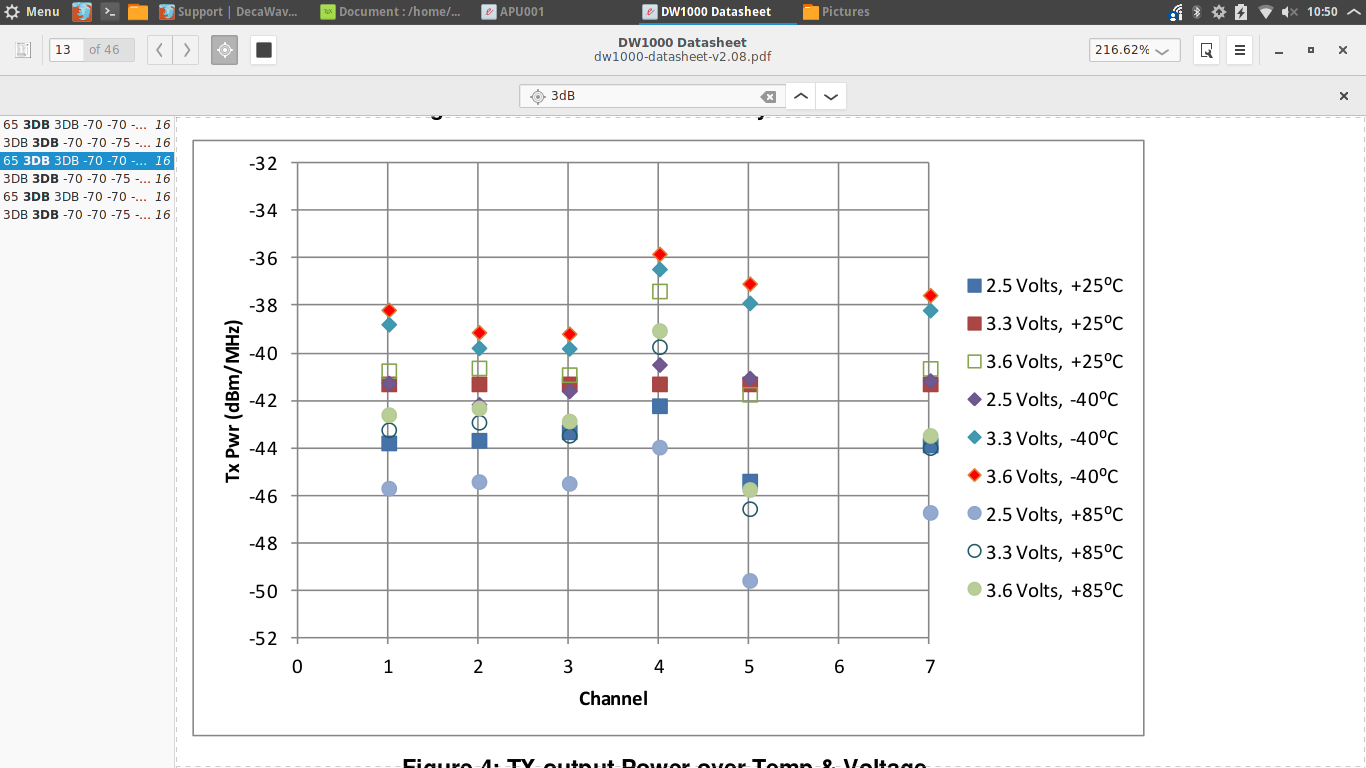
\includegraphics[scale=0.35,trim={7cm 1.5cm 8cm 5.5cm},clip]{data/tx_power.png}
\caption{TX Power vs Supply Voltage and Temperature.\cite{DW-data}}
\label{fig:tx-power}
\end{center}
\end{figure}

Figure~\ref{fig:tx-power} above shows that both the supply voltage and environmental temperature have an affect on the effective transmit power achieved. This means proper supply voltage regulation, as well as temperature regulation, are needed to ensure the transmit-receive performance designed for is achieved in practise.

\subsubsection{Bill of Materials}
\lsec{Tag BOM}
The bill of materials as well as unit pricing for the tag can be found in Appendix F. Where parts with specific tolerance, such as for the RF circuitry, are needed they have been ordered specifically. The non-critical parts were chosen to optimize the end unit price. 

All parts were ordered from Mouser except if specified otherwise. They offer international shipping and are a reliable source of components to minimize risk. The LiPo batteries were ordered from a chinese source, as stated in the BOM, and the supplier will need to be managed properly to reduce risk.

\textbf{The result of the BOM and Unit Cost analysis is the following:}

Total Capital Outlay (ZAR): R3558254 (tags) + R360000 (beacons)\\
Unit Cost for Tags (ZAR): R237 (circuitry) + R180 (casing)
Unit Cost for Beacons (ZAR): R12000

It was decided not to include the BOM and Unit Cost analysis for the beacons, as their costs will be minimal when compared with the 15000 tags needed for the system. The estimated cost for the beacon, as seen in the Mechanical Design section, was R12000 per beacon. With 30 beacons distributed across the upper campus parking areas, this works out to R360000. In terms of circuitry, the beacons will work out to the same price as a tag - adding WiFi but not using LiPo batteries. There will be the additional expense of the following: WiFi chips, beacon platform, beacon power supplies, high gain antenna. 

\newpage
\subsection{Assumptions}
The following assumptions were made and validated as indicated:

\begin{enumerate}
\item \textbf{Solar panels are able to provide the needed power for recharge of the LiPo batteries.}\\The circuitry of the chips is protected with a casing which is placed inside the vehicles, this ensures disturbances and damages are minimized.
\item \textbf{Five hours of sunlight expected at beacon locations.}\\The location chosen from the map for beacon placement are in direct sunlight, no obstruction from trees or buildings.
\item \textbf{Circuitry components will have correct (and within ratings) voltage levels.}\\Voltage ratings of the circuits are studied and necessary regulators used to ensure maintenance of the correct voltage at all times and the system designed to protect itself from overload 
\item \textbf{The beacons’ transceiver chips will not be vandalized or disrupted.}\\The height of the beacons is just over nine metres, and the chips are placed at the highest point which brings difficulty in accessibility. The height also helps in the operation range of the tag antenna choice. 
\item \textbf{Triangulation method will always provide accurate results.}\\Triangulation typical needs three beacons, the system is design to use four to ensure accuracy as well as a fail-sage mechanism
\item \textbf{Durability of the transceiver chips is certain.}\\The circuitry of the chips is protected with a casing which is placed inside the vehicles, this ensures disturbances and damages are minimized.
\item \textbf{Chip holders will comply by rules and not damage the transceiver chips.}\\The material for the chip casing cannot be easily damaged. The bar coded stick is needed for identification, therefore in order to avoid possible fines; users are encouraged to avoid tampering
\item \textbf{Constant rate of manufacturing prices.}\\Minimum laser cutting and material costs’ estimation for system have been based on Pololu Robotics and Electronics and Robor Steel pricings with constant market-based inflation rate of 1\% 
And 4.82\% respectively.
\end{enumerate}

\newpage
\subsection{Failure Modes}
The following table discusses the failure mode effect analysis (FMEA) of the system.\cite{FMEA} 

The rating scores are as follows:

1=not severe, 10=very severe; \\
1=not likely, 10=very likely; \\
1=easy to detect, 10=not easy to detect. \\

\begin{figure}[H]
\begin{center}
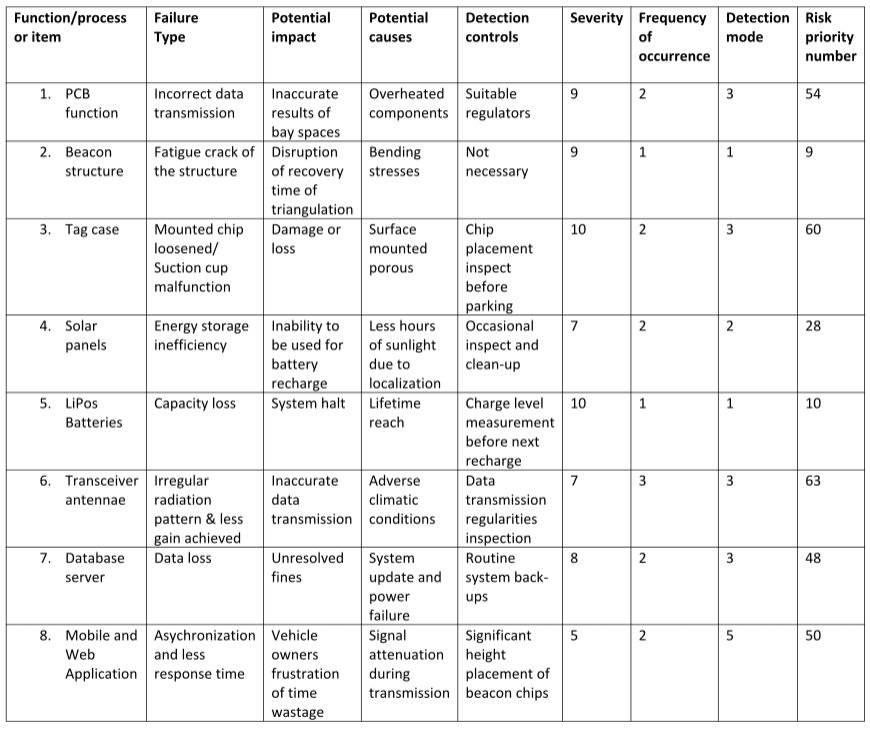
\includegraphics[scale=0.6]{data/failure-modes.png}
\caption{Failure mode effect analysis.}
\label{fig:failure}
\end{center}
\end{figure}

%\begin{table}[H]
%\centering
%\begin{tabular}{|p{3cm}|p{3cm}|p{3cm}|p{3cm}|p{3cm}|p{1.5cm}|p{1.5cm}|p{1.5cm}|p{1.5cm}|}
%\hline
%\textbf{Function / processor item}    & \textbf{Failure Type}                              & \textbf{Potential impact}                    & \textbf{Potential causes}                  & \textbf{Detection}                   & \textbf{Severity} & \textbf{Frequency} & \textbf{Detection mode} & \textbf{Risk priority} \\ \hline
%\textbf{PCB function}               & Incorrect data transmission                       & Inaccurate results of bay spaces             & Overheated components                      & Suitable regulators                           & 9                 & 2                                & 3                       & 54                            \\ \hline
%\textbf{Beacon structure}           & Fatigue crack of the structure                    & Disruption of recovery time of triangulation & Bending stresses                           & Not necessary                                 & 9                 & 1                                & 1                       & 9                             \\ \hline
%\textbf{Tag case}                   & Mounted chip loosened/ Suction cup malfunction    & Damage or loss                               & Surface mounted porous                     & Chip placement inspect before parking         & 10                & 2                                & 3                       & 60                            \\ \hline
%\textbf{Solar panels}               & Energy storage inefficiency                       & Inability to be used for battery recharge    & Less hours of sunlight due to localization & Occasional inspect and clean-up               & 7                 & 2                                & 2                       & 28                            \\ \hline
%\textbf{LiPo Batteries}            & Capacity loss                                     & System halt                                  & Lifetime reach                             & Charge level measurement before next recharge & 10                & 1                                & 1                       & 10                            \\ \hline
%\textbf{Transceiver antennae}       & Irregular radiation pattern \& less gain achieved & Inaccurate data transmission                 & Adverse climatic conditions                & Data transmission regularities inspection     & 7                 & 3                                & 3                       & 63                            \\ \hline
%\textbf{Database server}            & Data loss                                         & Unresolved fines                             & System update and power failure            & Routine system back-ups                       & 8                 & 2                                & 3                       & 48                            \\ \hline
%\textbf{Mobile and Web Application} & Asychronization and less response time            & Vehicle owners frustration of time wastage   & Signal attenuation during transmission     & Significant height placement of beacon chips  & 5                 & 2                                & 5                       & 50                            \\ \hline
%\end{tabular}
%\caption{Failure mode effect analysis.}
%\label{my-label}
%\end{table}


\newpage
\subsection{System Lifetime}
The design lifetime of the system is expected to be 15 years, with certain sub-systems requiring more regular replacement. 

The sub-systems that will limit the design lifetime are the following:
\begin{itemize}
\item \textbf{LiPo Batteries:} LiPo batteries will need to be replaced every year for the beacons and every 5 years for the tags. The 5 year lifetime of the tag is due to exposure to heat rather than exceeding the charge cycle limit, as they will be charged once a year upon return from the user. 
\item \textbf{Tags:} The tags will be in an unknown environment. This could lead to mishandling by the users and possible damage - these will need to be replaced.
\item \textbf{Solar Panel:} Solar panels in outdoor environments need to be maintained and possibly replaced every 15 years. 
\end{itemize}

\subsection{Worst Case Calculation}
This section will focus on the factors affecting the distance measurement from the tags to the beacons,
and the worst case distance error that can result. The value of the distance measurement was chosen
for this analysis because it is at the core of the system. The distance measurements are what determine
the accuracy of the determination of the location of a tag. The accuracy of the location estimate, in turn,
affects how effective the system is at determining which parking bays are occupied. The simulation
described in section~\ref{sim} allows for the assessment of the effect of distance error on the accuracy of
the parking bay occupation algorithm. Table~\ref{tbl:dst-error} shows the sources of error and their estimated
magnitude.

\begin{table}[H]
\centering
\begin{tabular}{|p{3cm}|p{3cm}|p{5cm}|}
\hline
\textbf{Factor}                        & \multicolumn{1}{l|}{\textbf{Introduced Distance Error}} & \multicolumn{1}{l|}{\textbf{Comment}}                                                                                                                                  \\ \hline
\textbf{Signal level}                  & $\pm 0.15 m$ \newline (Uncompensated) $\pm 0.05 m$ \newline (Compensated)            & Can be compensated for using Friis’ path loss formula.\cite{2} Then the error can be taken to be much smaller, perhaps a worst case of $0.05 m$.                          \\ \hline
\textbf{Attenuation through vehicles}  & $+1 \%$ (Estimate)                                        & Cannot be factored into path loss compensation because the attenuation depends on the vehicles parked nearby. Can be minimised by having beacons at sufficient height. \\ \hline
\textbf{Noise and interference from other tags} & $\pm 0.5 \%$ \newline (Estimate)                                      & Not a significant issue with the Ultra Wide Band DecaWave chips.\cite{gaffney}                                                                                               \\ \hline
\end{tabular}
\caption{Sources of error in the distance measurement.}
\label{tbl:dst-error}
\end{table}

The resulting worst case error is therefore
\begin{equation*}
\begin{split}
Worst Case Error &= +1\% + 0.5\% + 0.05 m \\
&= +1.5\% + 0.05 m
\end{split}
\end{equation*}
Knowing that each parking area will be served by a minimum of 4 beacons, and based on the size of
parking areas at UCT, it can be said that no parking spot will be more than 50 m away from any of the 3
nearest beacons. The absolute worst case error is then
\begin{equation*}
\begin{split}
Worst Case Error &= 50 \times 1.5\% + 0.05 m \\
&= 0.8 m
\end{split}
\end{equation*}
The simulation in section~\ref{sim} showed that the distance error cut-off point was at $\pm 0.5m$ before a
poorly parked car was detected to be in the wrong bay. However, this is assuming equal distance error
at each beacon, which is not the case in reality, where one beacon will be the furthest away, while the other two will be nearer, resulting in this worst case distance error only applying to one of the three
nearest beacons. Thus, it can be said that the system should be accurate enough even in the worst case.

If further testing shows that the error is in fact too great, the tag distance to the nearest three beacons
can easily be decreased by simply adding another one or two beacons to the parking area. This can be
done without increasing the cost of the system too much due to the relatively low cost of the beacons.

\textit{Report structure compiled from class notes.}\cite{handout}\cite{notes}

%\begin{figure}[H]
%\begin{center}
%\includegraphics[trim={Lcm Bcm Rcm Tcm},clip]{images/Fig1.pdf}
%\caption{•}
%\end{center}
%\end{figure}

%\begin{minted}[linenos=true]{matlab}
%\end{minted}

%######################Appendices######################
\newpage
\vspace*{\fill}
\begin{center}
\subsection*{Appendix A: Contributions}
\end{center}
\vspace*{\fill}
\addcontentsline{toc}{section}{Appendix A: Contributions}

\newpage
\subsubsection*{Jarushen Govender (GVNJAR002)}
5. Conceptual Design: Design Two.\\
6. Embodiment Design: Power Requirements.\\
Progress Report 3.
\subsubsection*{Isaac Lebogang Khobo (KHBISA001)}
6. Embodiment Design: Mechanical Design, Assumptions, Failure Modes.\\
Progress Report 4. \\
Appendix G1, G2.
\subsubsection*{Benjamin Scholtz (SCHBEN011)}
LATEX Formatting/Template. \\
2. Task Clarification. \\
3. Context of Design. \\
4. Design Specification. \\
5. Conceptual Design: Design One, Weighted Selection, Recommendation. \\
6. Embodiment Design: Schematics (Tag and Beacon), PCB Design (Tag and Beacon), RF Design, Bill of Materials (Tag), System Lifetime. \\
Progress Report 2. \\
Appendix C,D,E,F.
\subsubsection*{Nasko Stavrev (STVATA001)}
Simulation.\\
6. Embodiment Design: System Overview, Software Design, Worst Case Calculation.

\vfill
\textbf{Note: }\textit{all team members contributed throughout the course of the design to the various sections mentioned - each section was compiled by the team member shown.}

\newpage
\vspace*{\fill}
\begin{center}
\subsection*{Appendix B: Progress Reports}
\end{center}
\vspace*{\fill}
\addcontentsline{toc}{section}{Appendix B: Progress Reports}

\newpage
\subsection*{Progress Report 1: SCHBEN011}
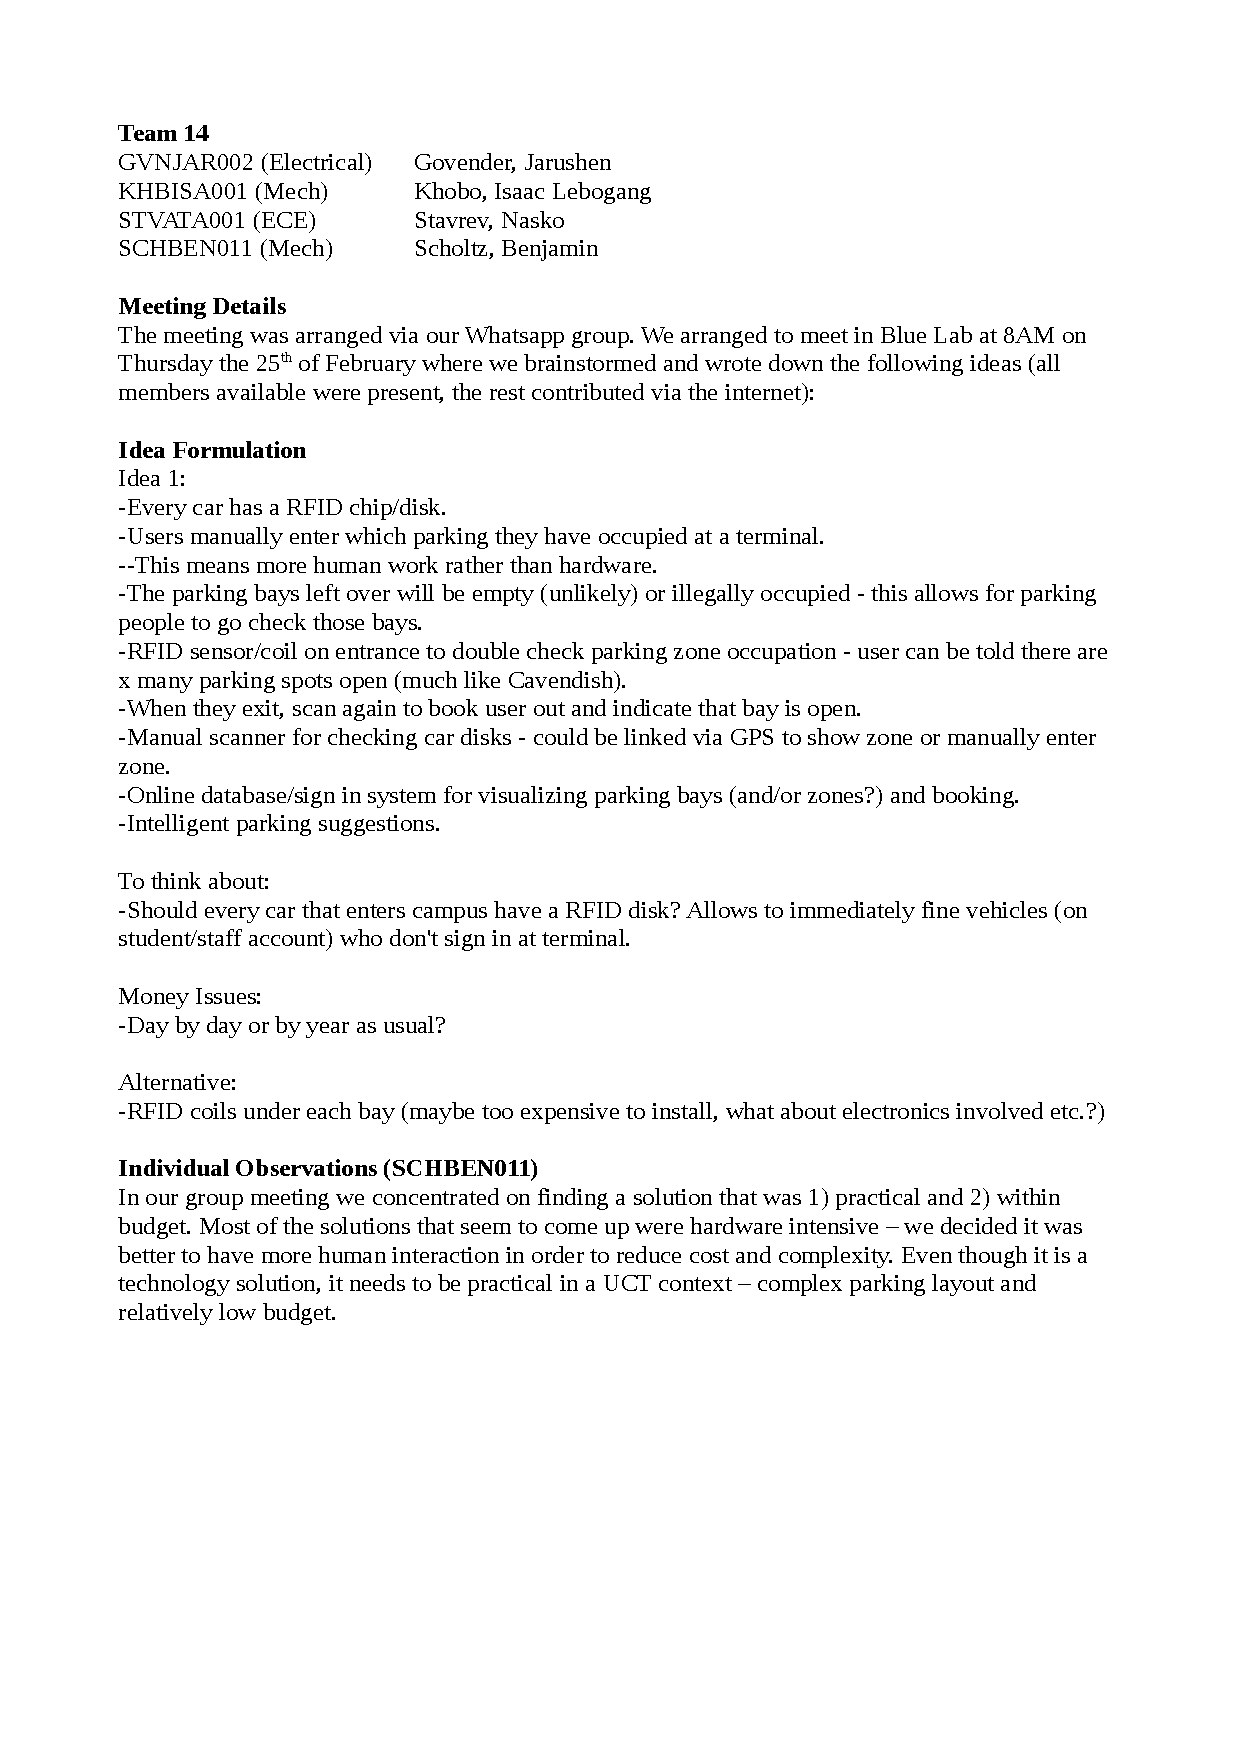
\includegraphics[scale=0.9]{meeting/report1-ben.pdf}

\newpage
\subsection*{Progress Report 1: STVATA001}
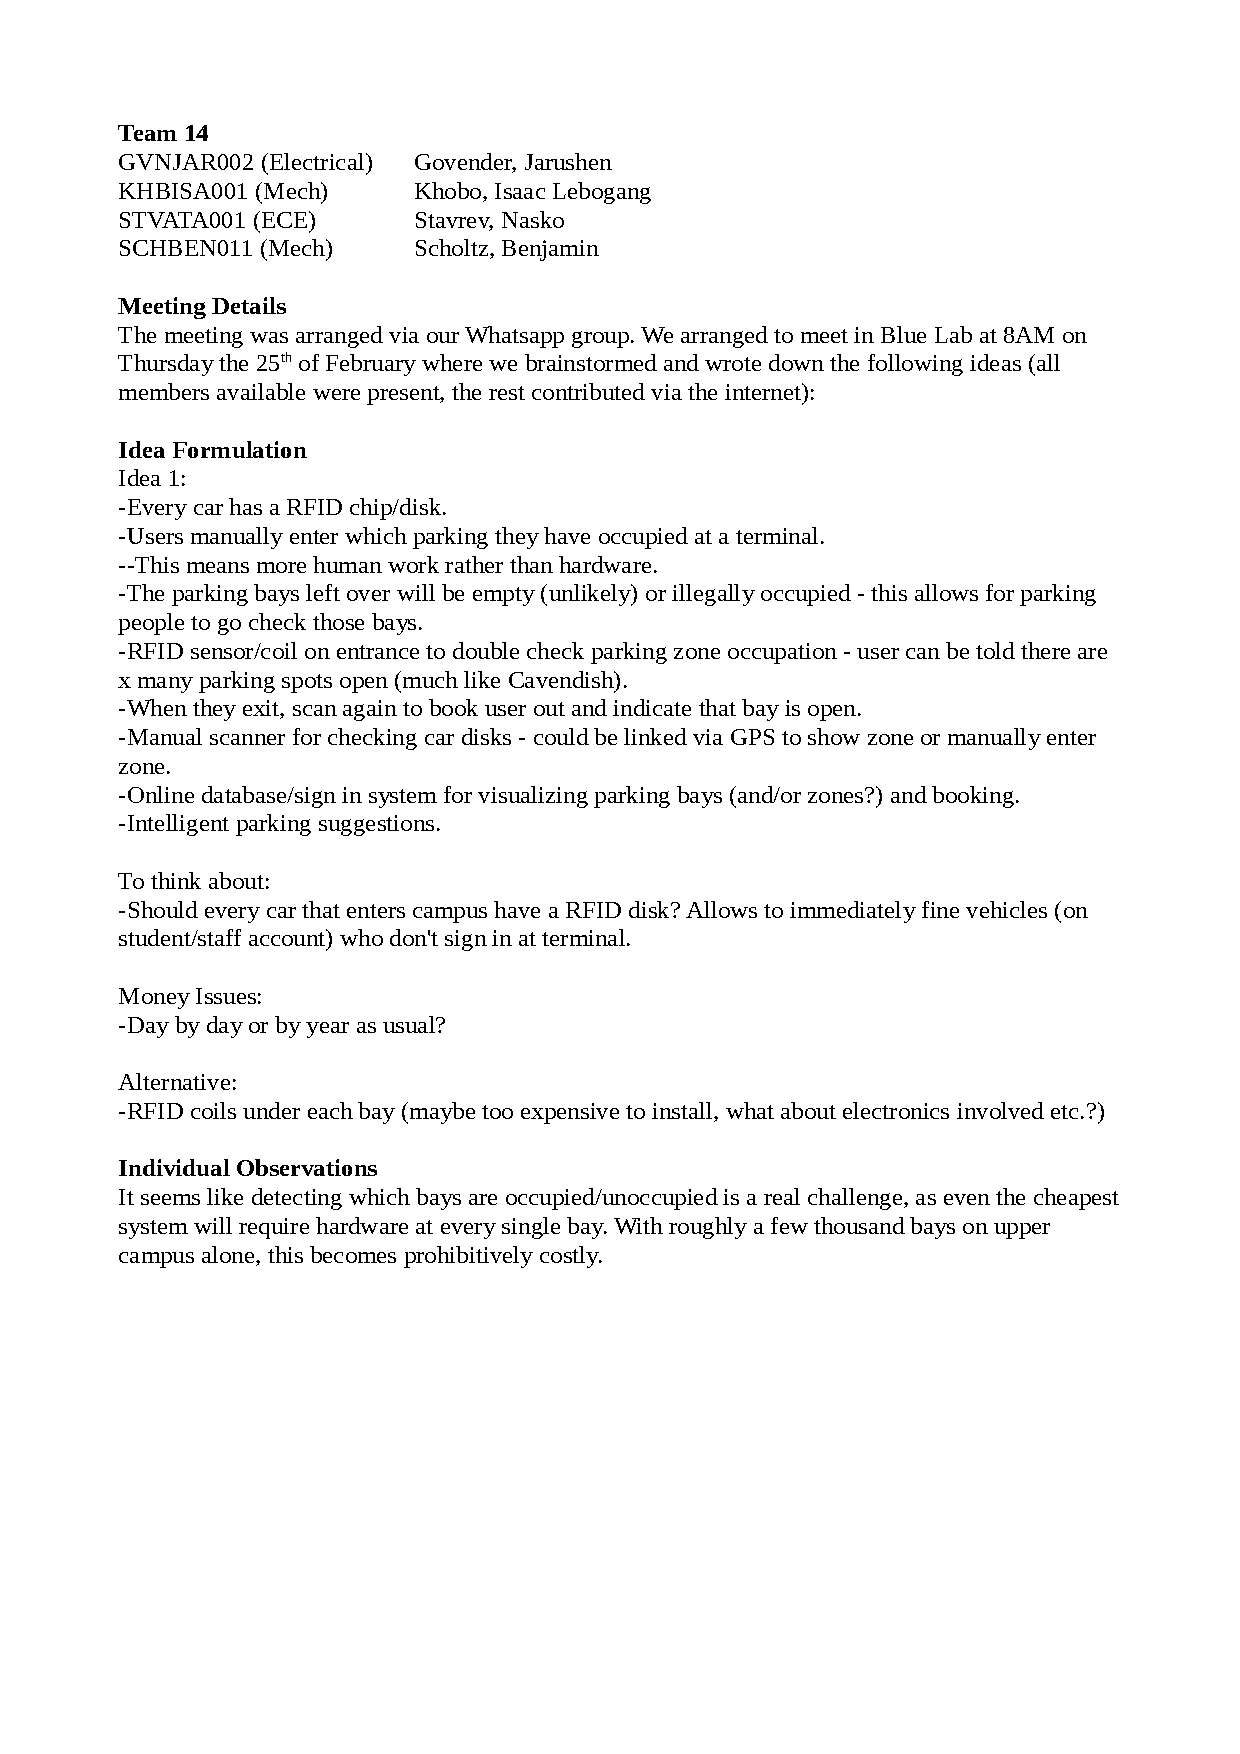
\includegraphics[scale=0.9]{meeting/report1-nasko.pdf}

\newpage
\subsection*{Progress Report 1: KHBISA001}
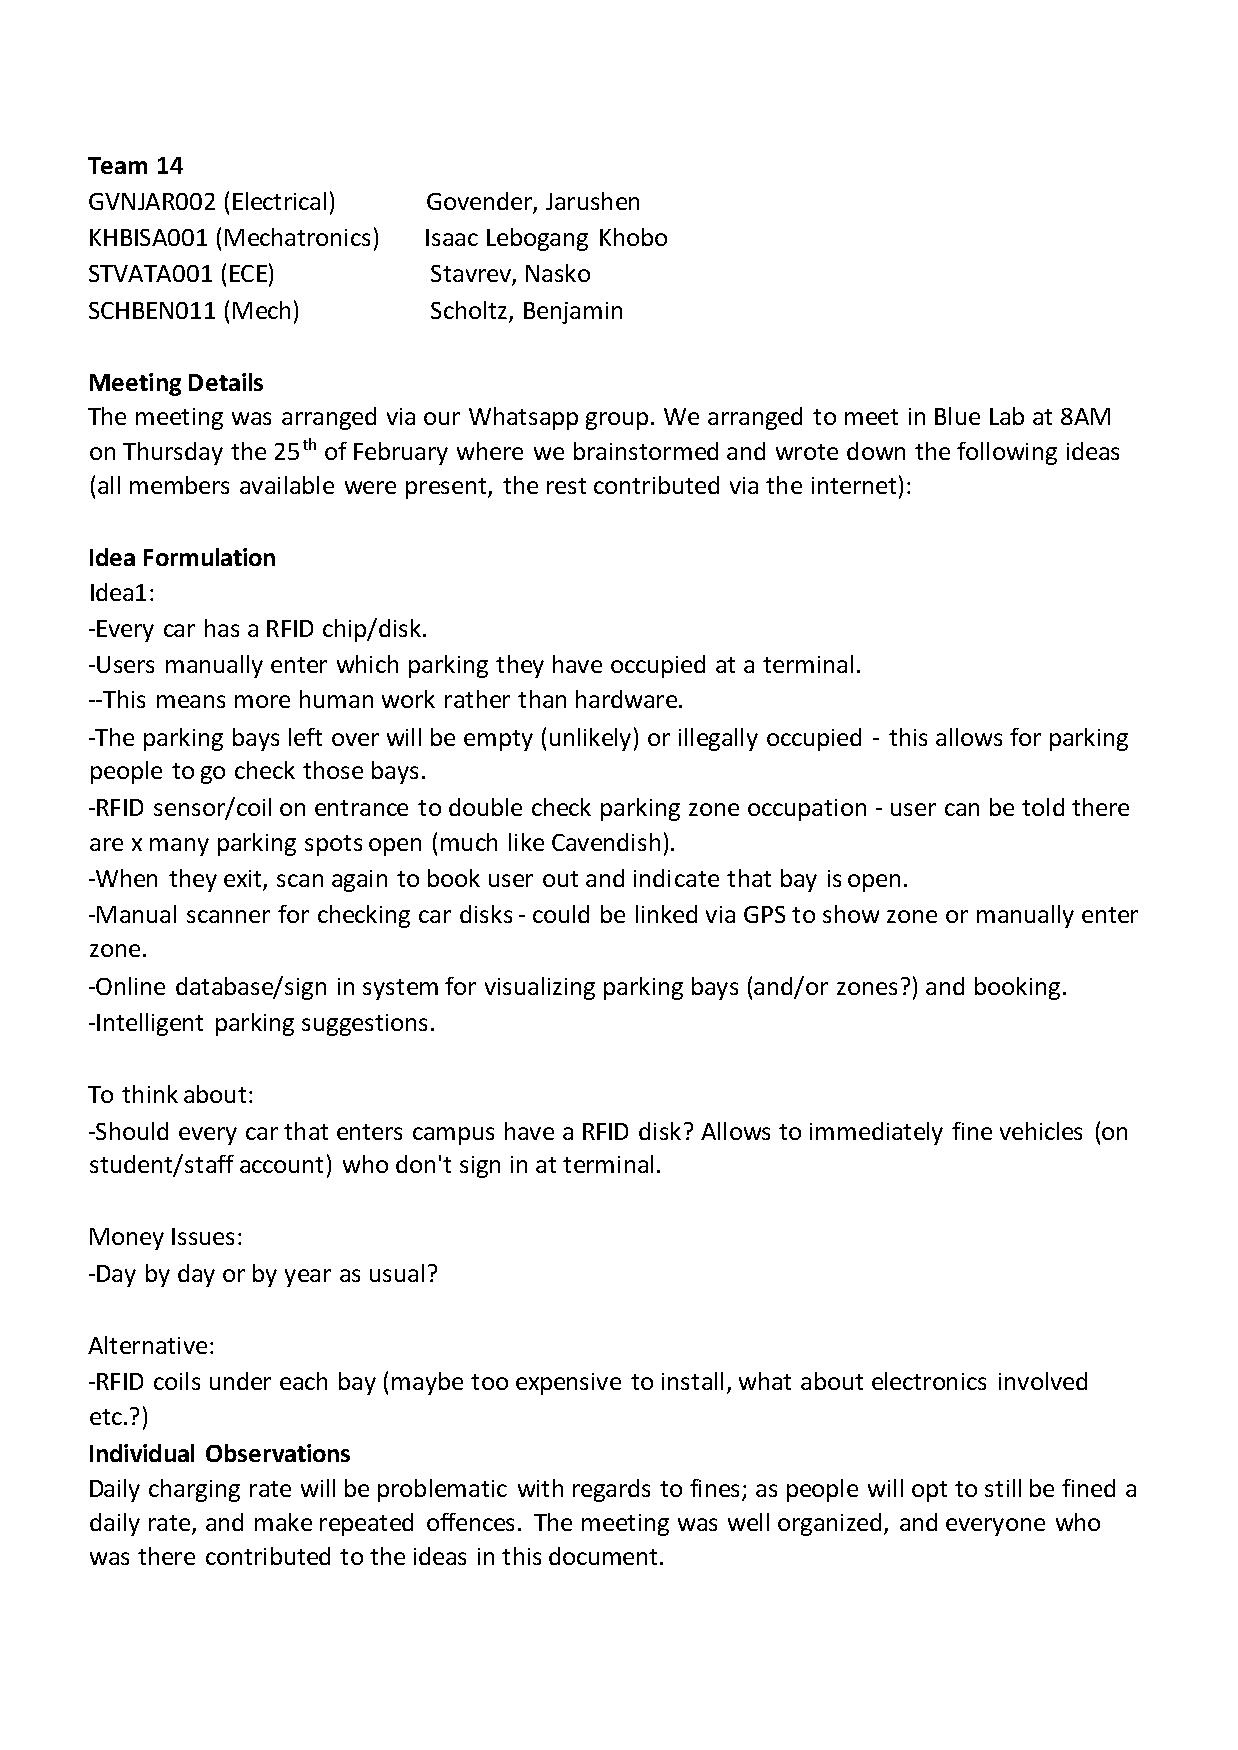
\includegraphics[scale=0.9]{meeting/report1-isaac.pdf}

\newpage
\subsection*{Progress Report 1: GVNJAR002}
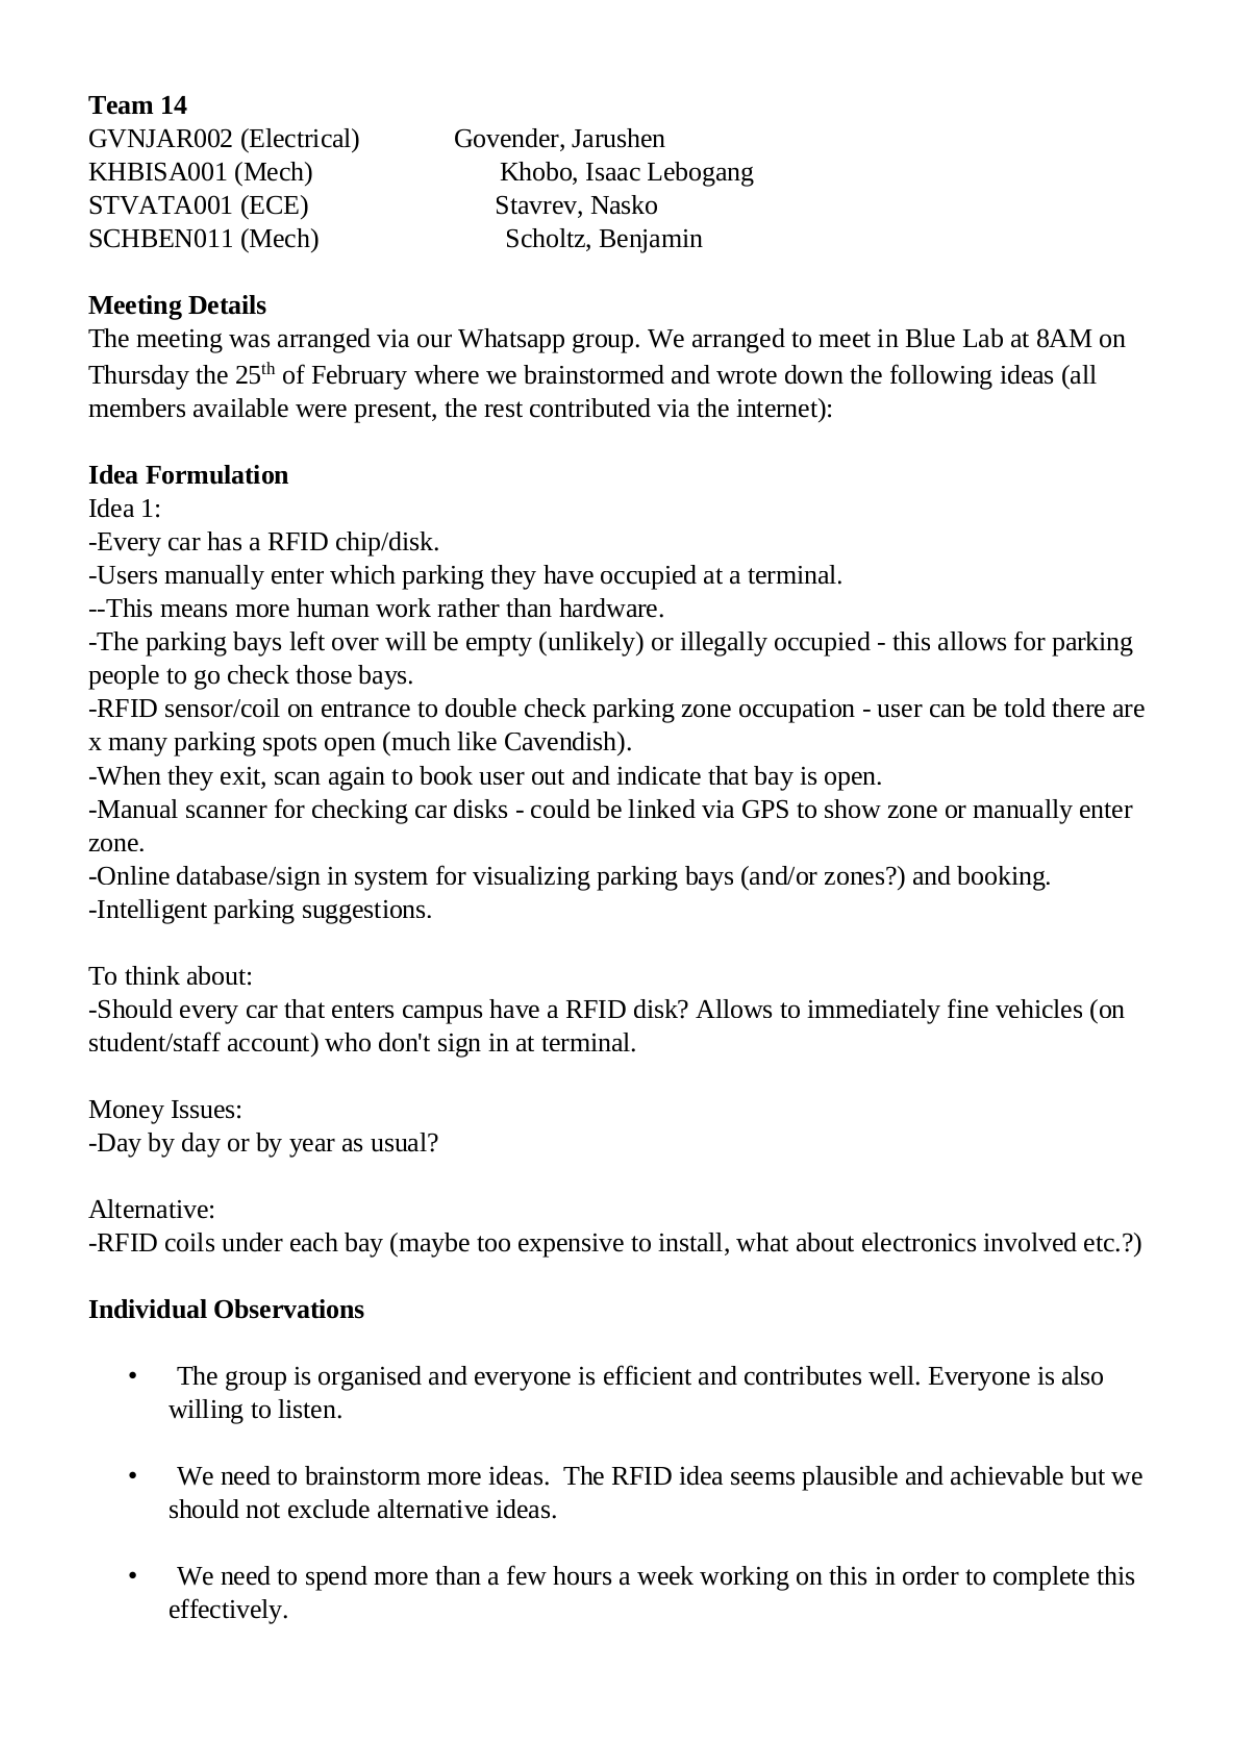
\includegraphics[scale=0.8]{meeting/report1-jarushen.pdf}

\newpage
\subsection*{Progress Report 2}
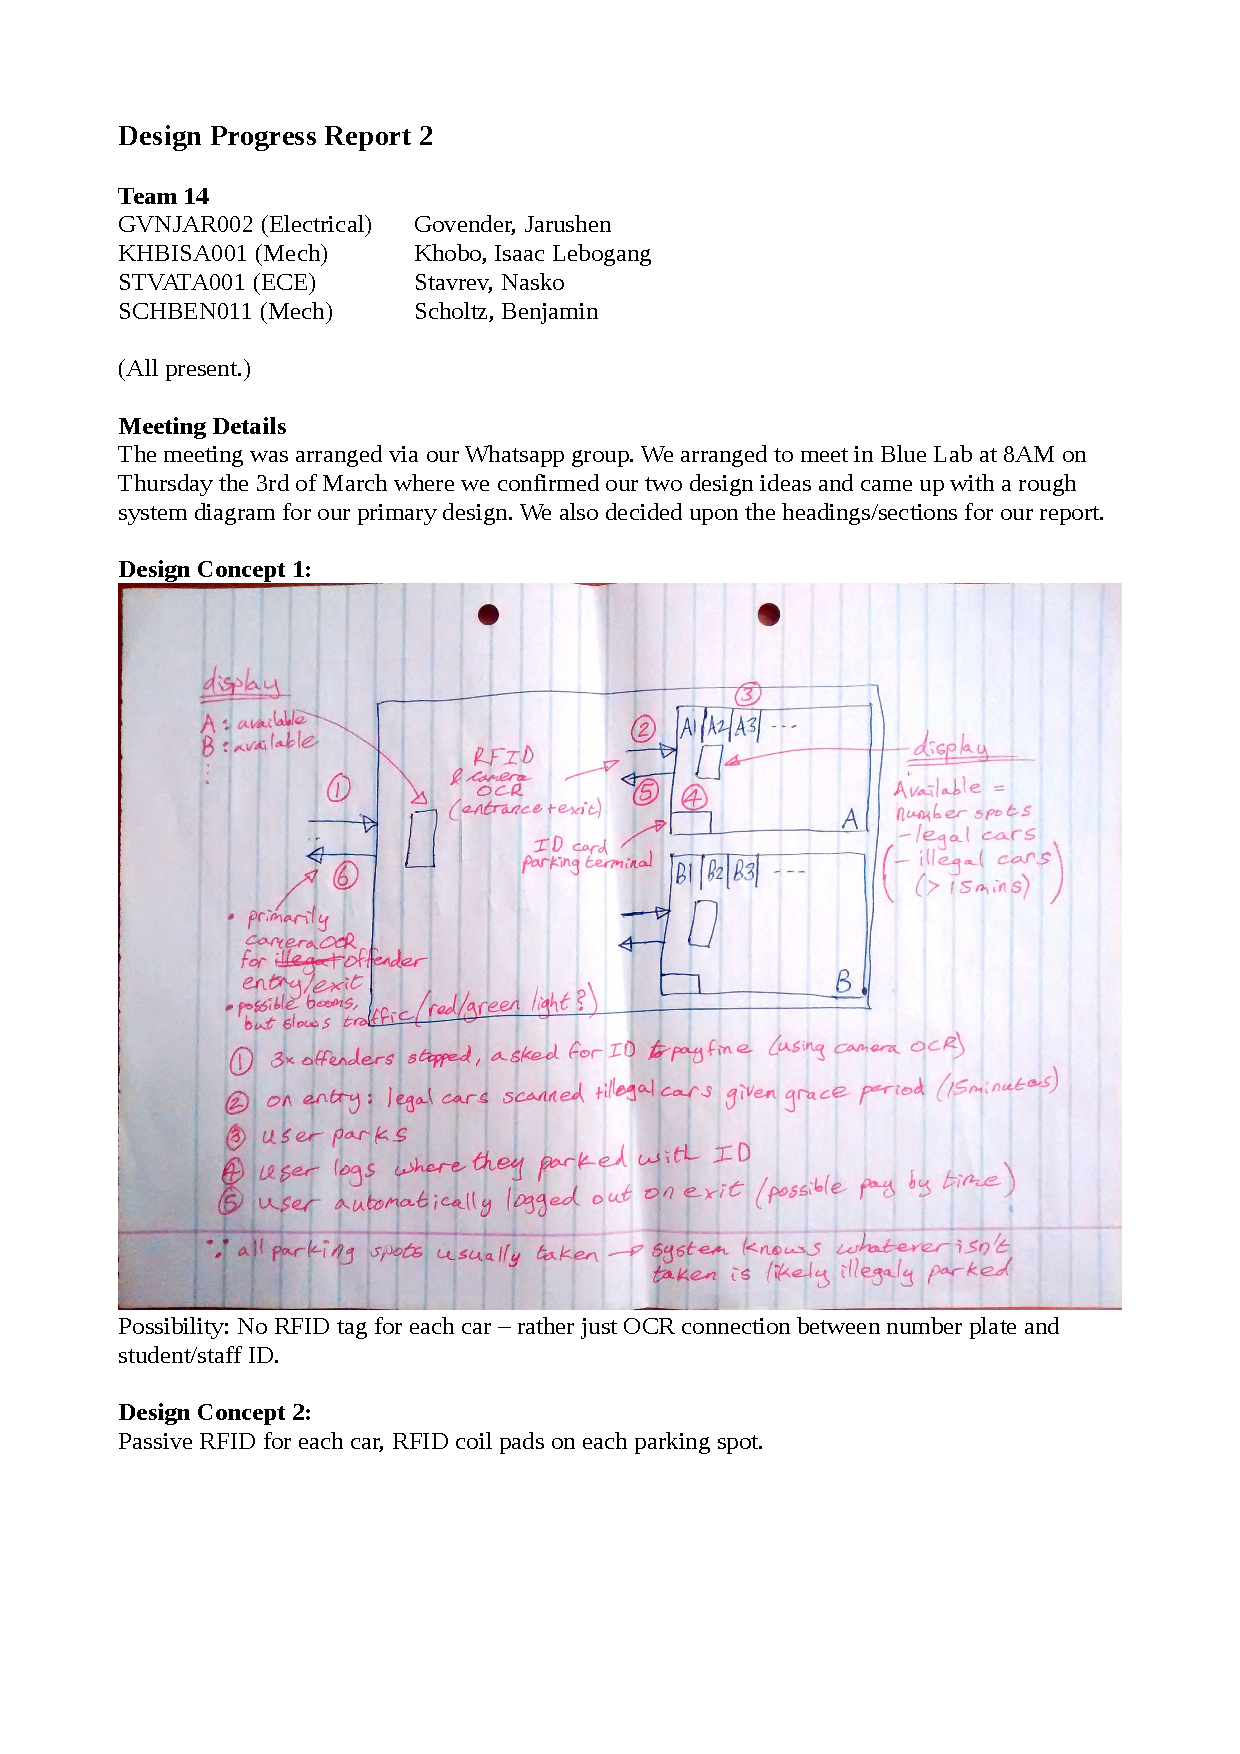
\includegraphics[scale=0.9]{meeting/report2-ben.pdf}
\includegraphics[page=2,scale=0.9]{meeting/report2-ben.pdf}

\newpage
\subsection*{Progress Report 3}
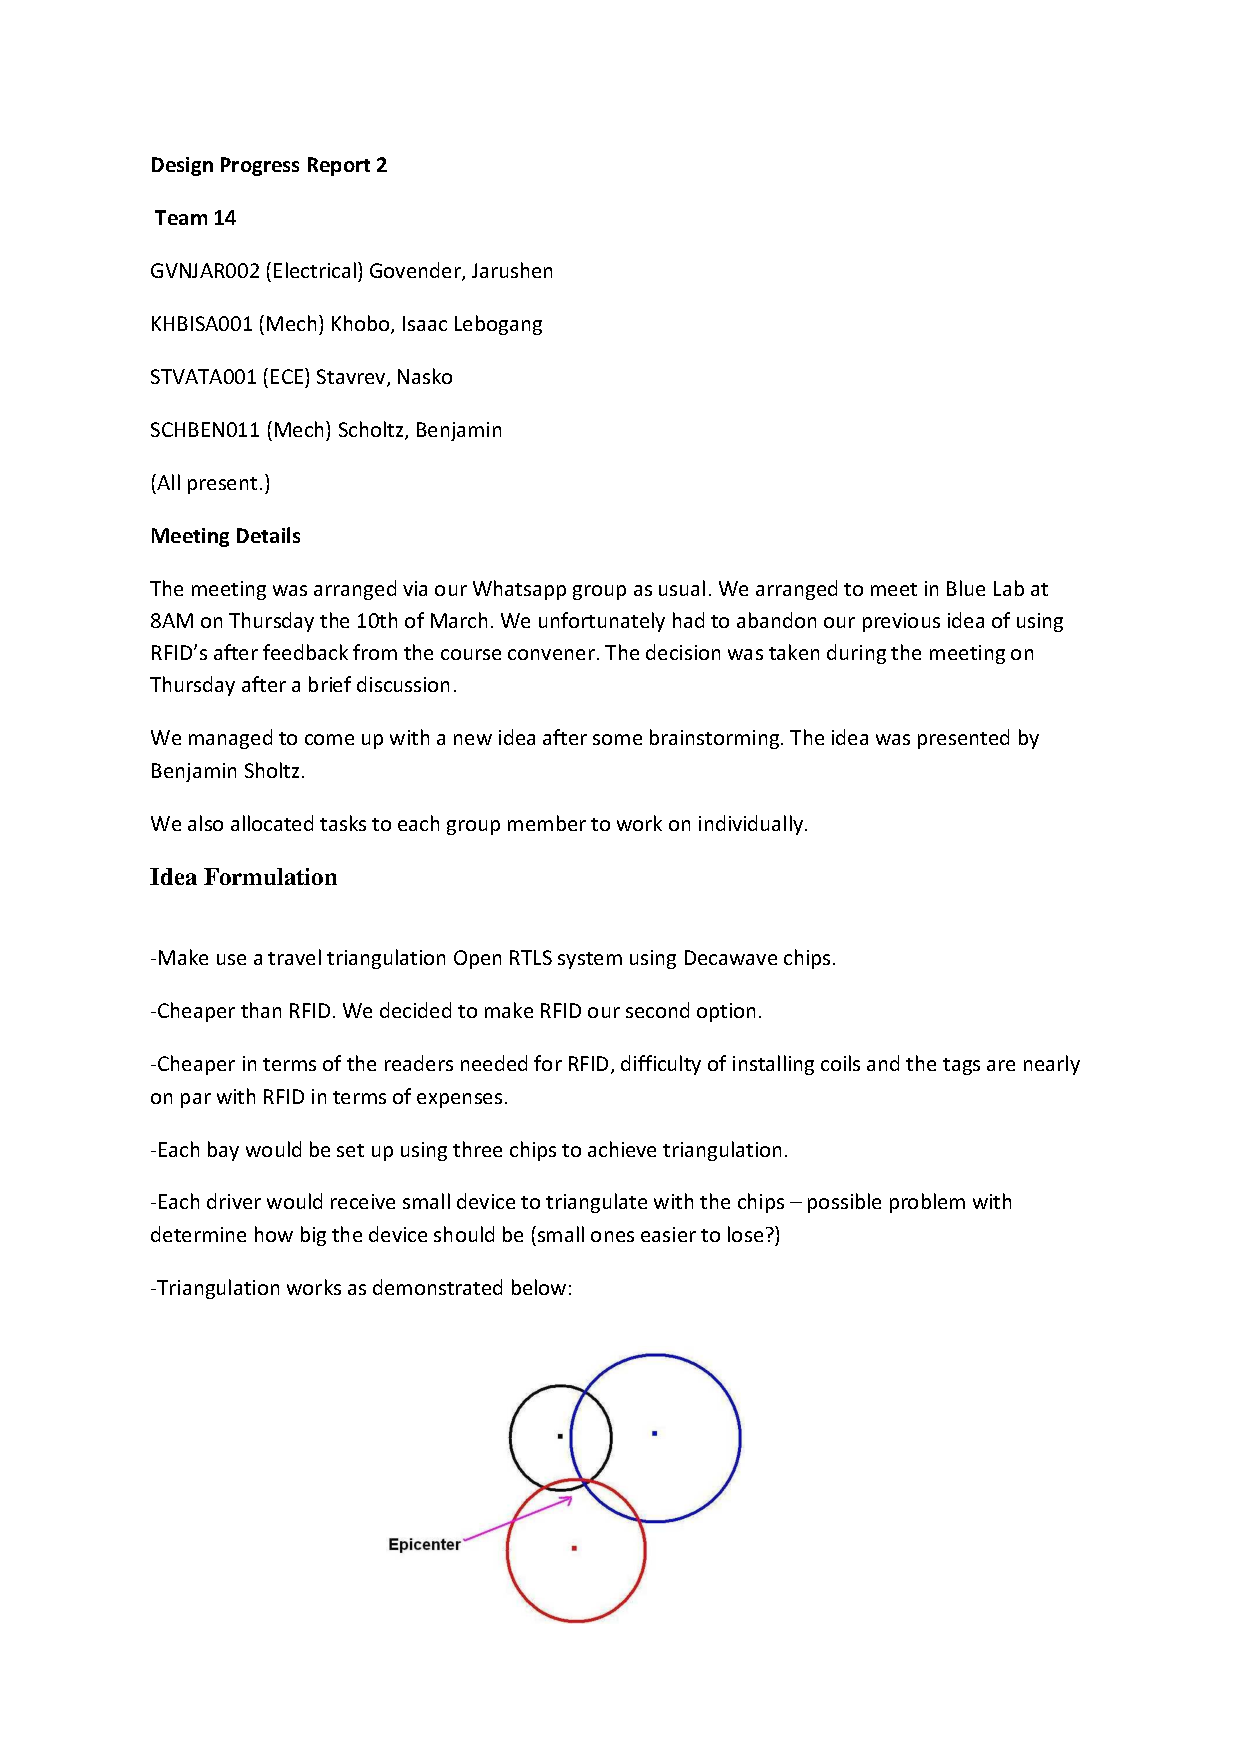
\includegraphics[scale=0.85]{meeting/report3-jarushen.pdf}\\
\includegraphics[page=2,scale=0.9]{meeting/report3-jarushen.pdf}
\includegraphics[page=3,scale=0.9]{meeting/report3-jarushen.pdf}

\newpage
\subsection*{Progress Report 4}
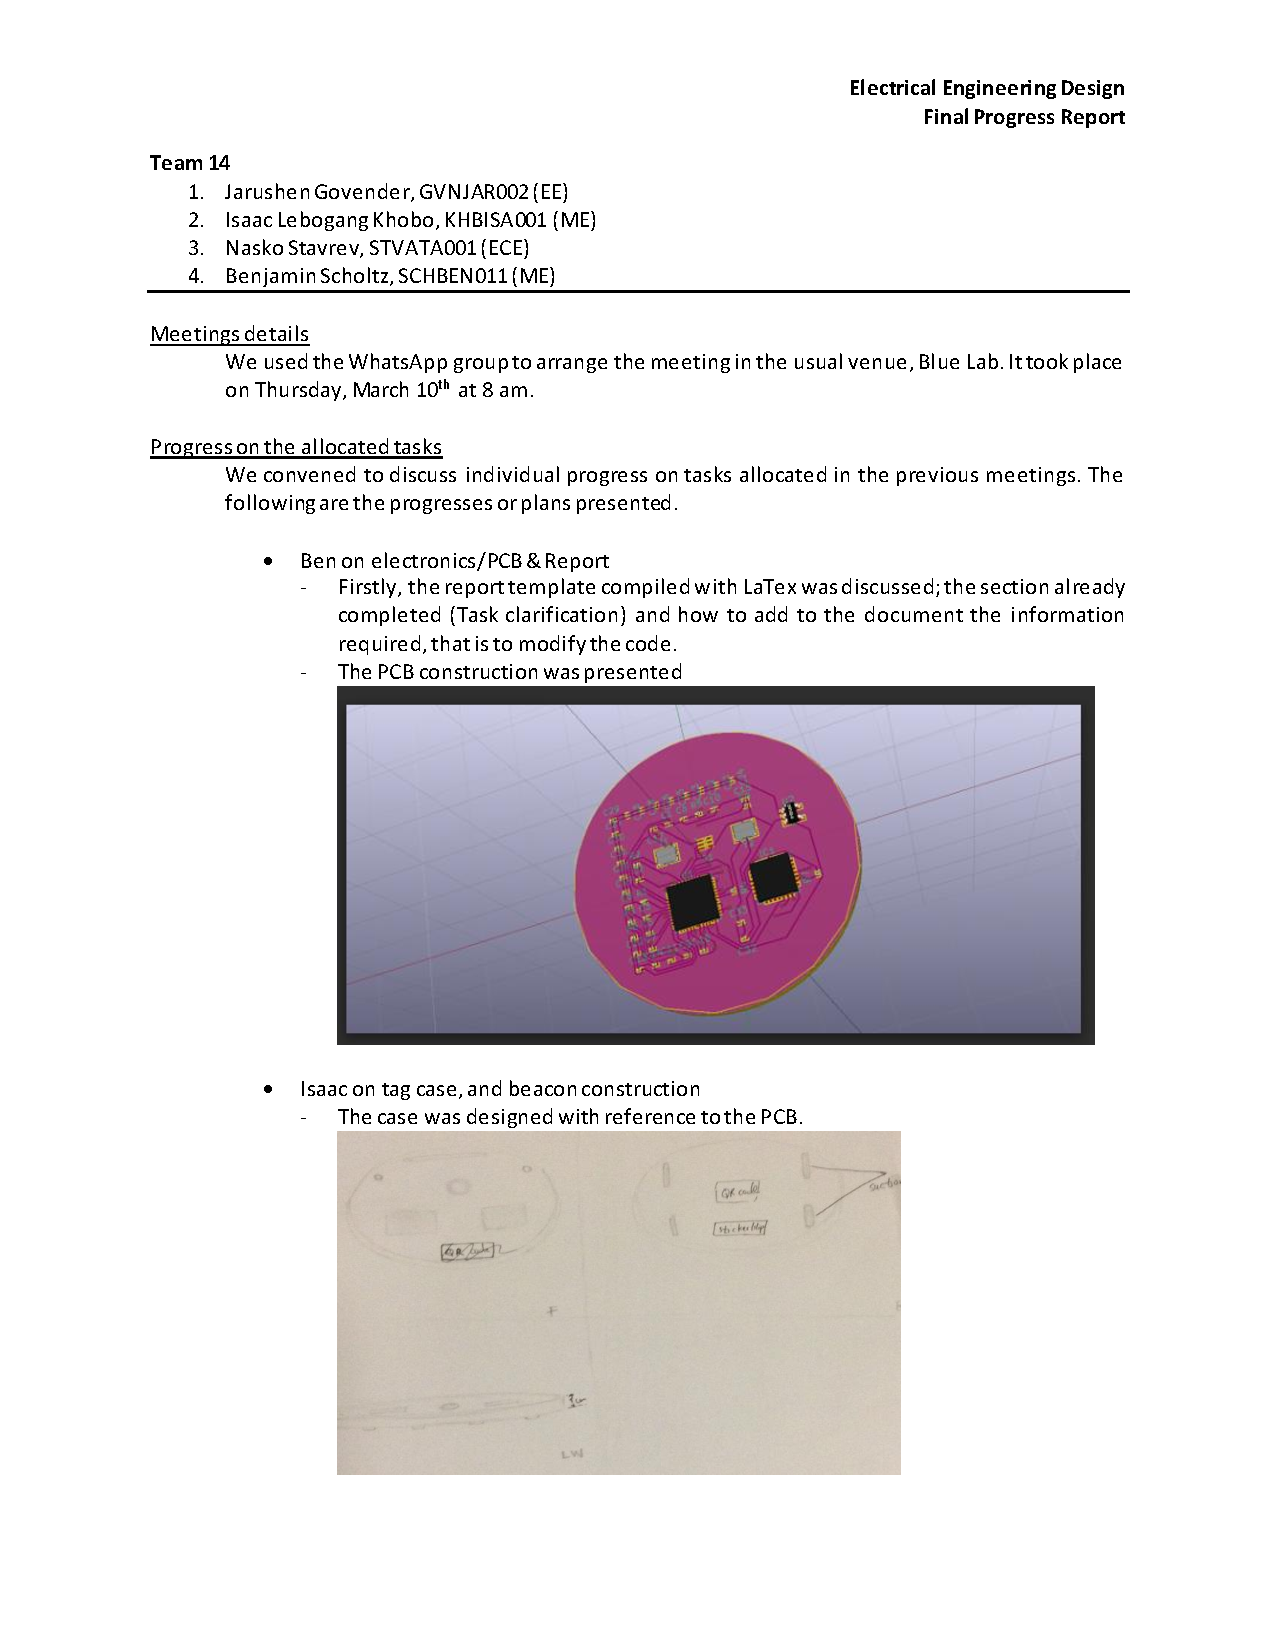
\includegraphics[scale=0.9]{meeting/report4-isaac.pdf}
\includegraphics[page=2,scale=0.9]{meeting/report4-isaac.pdf}
\includegraphics[page=3,scale=0.9]{meeting/report4-isaac.pdf}


\newpage
\vspace*{\fill}
\begin{center}
\subsection*{Appendix C: Tag Schematic Diagram}
\end{center}
\vspace*{\fill}
\addcontentsline{toc}{section}{Appendix C: Tag Schematic Diagram}
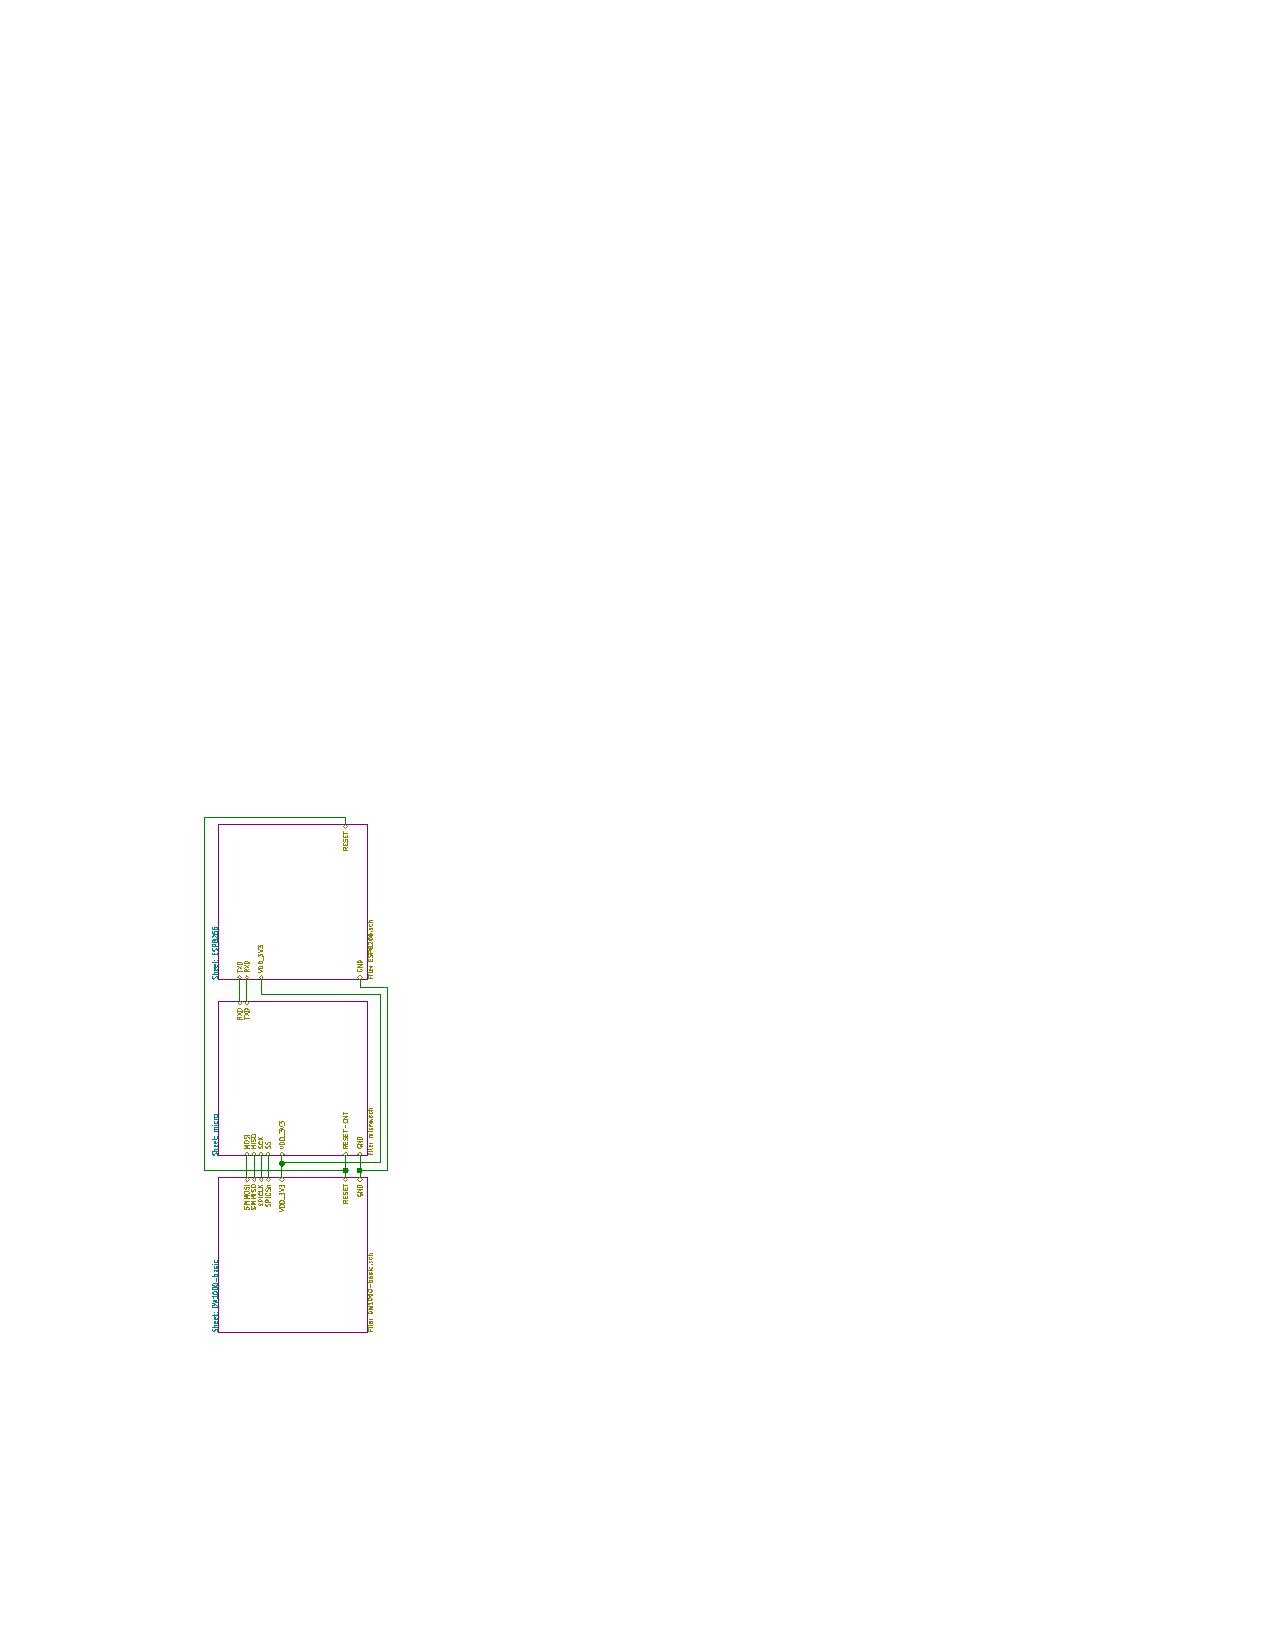
\includepdf[pages=-]{data/parking-system2.pdf}

\newpage
\vspace*{\fill}
\begin{center}
\subsection*{Appendix D: Tag PCB Layout}
\end{center}
\vspace*{\fill}
\addcontentsline{toc}{section}{Appendix D: Tag PCB Layout}
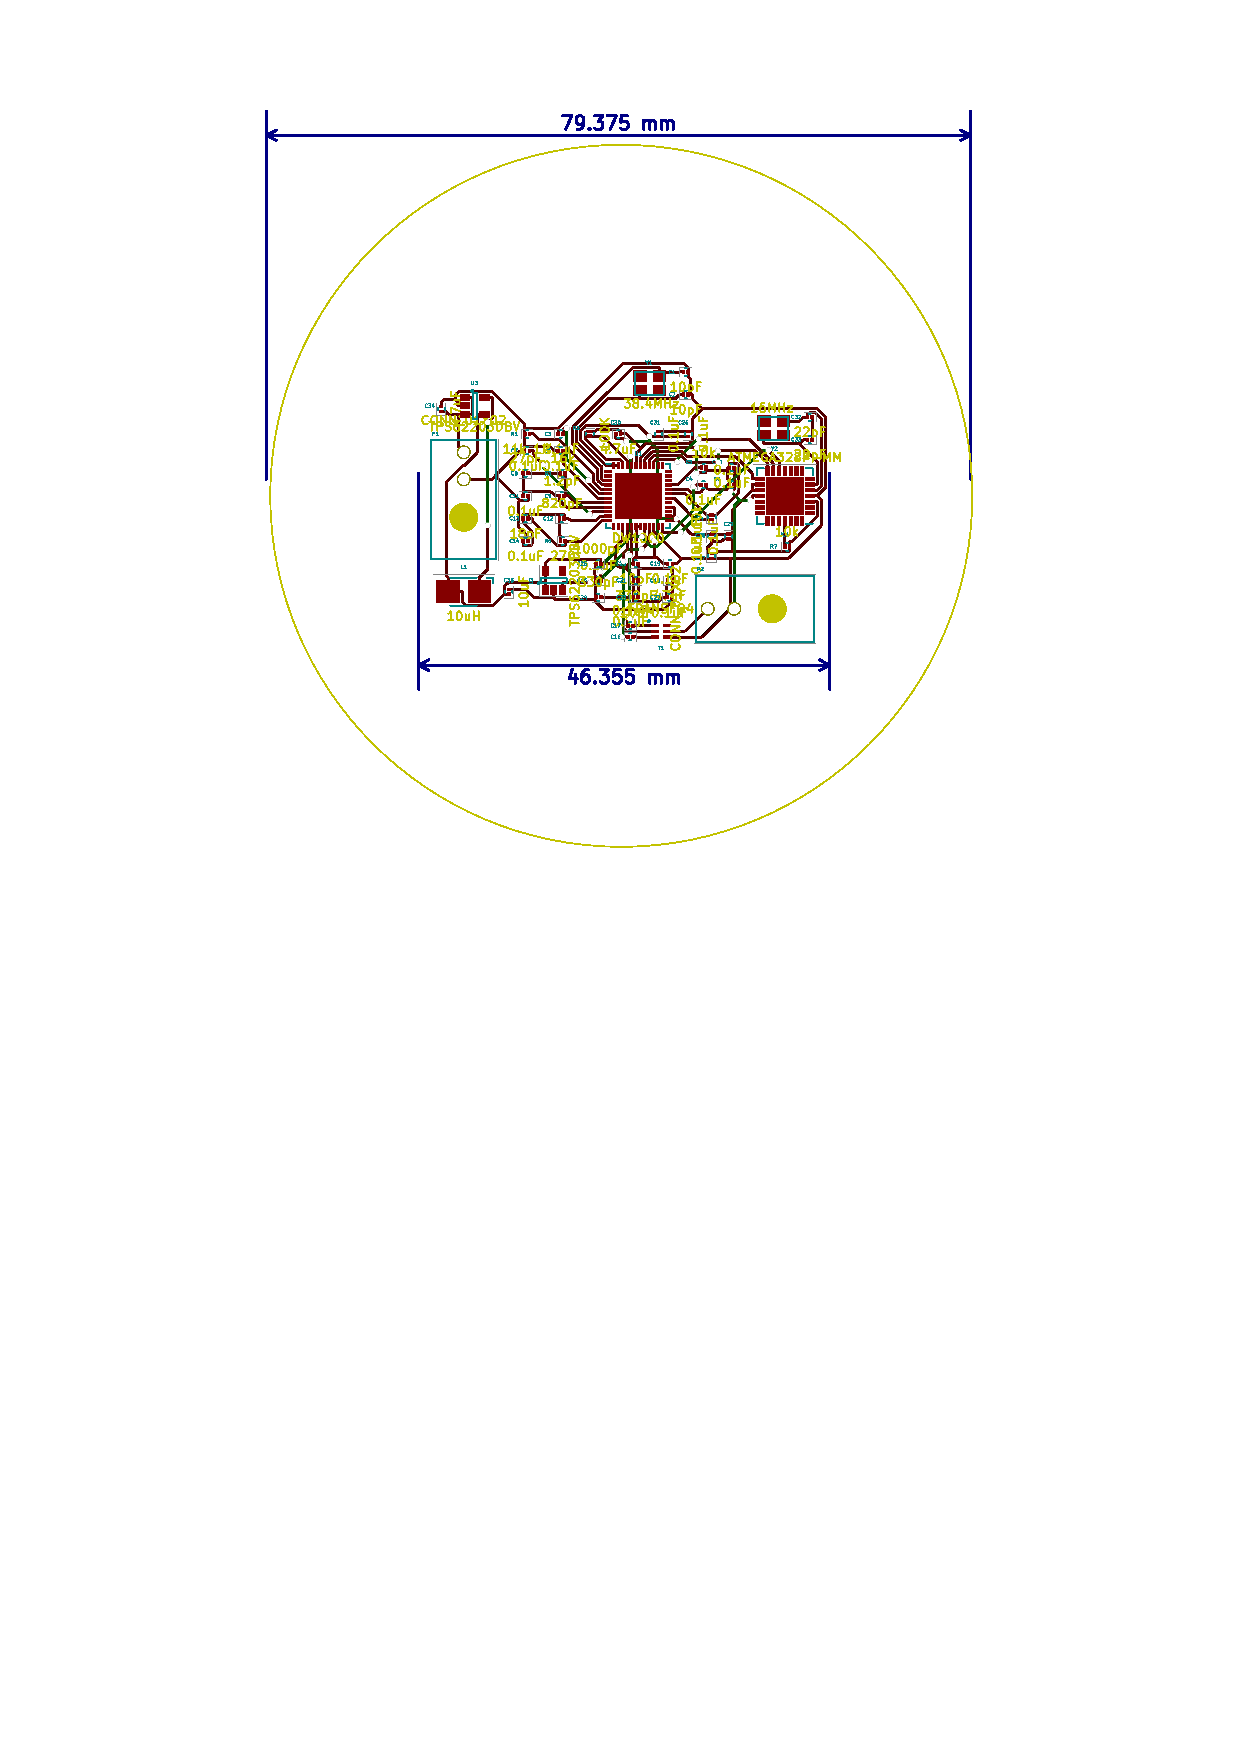
\includepdf[pages=-]{data/pcb-layout.pdf}

\newpage
\vspace*{\fill}
\begin{center}
\subsection*{Appendix E: Beacon PCB Layout}
\end{center}
\vspace*{\fill}
\addcontentsline{toc}{section}{Appendix E: Beacon PCB Layout}
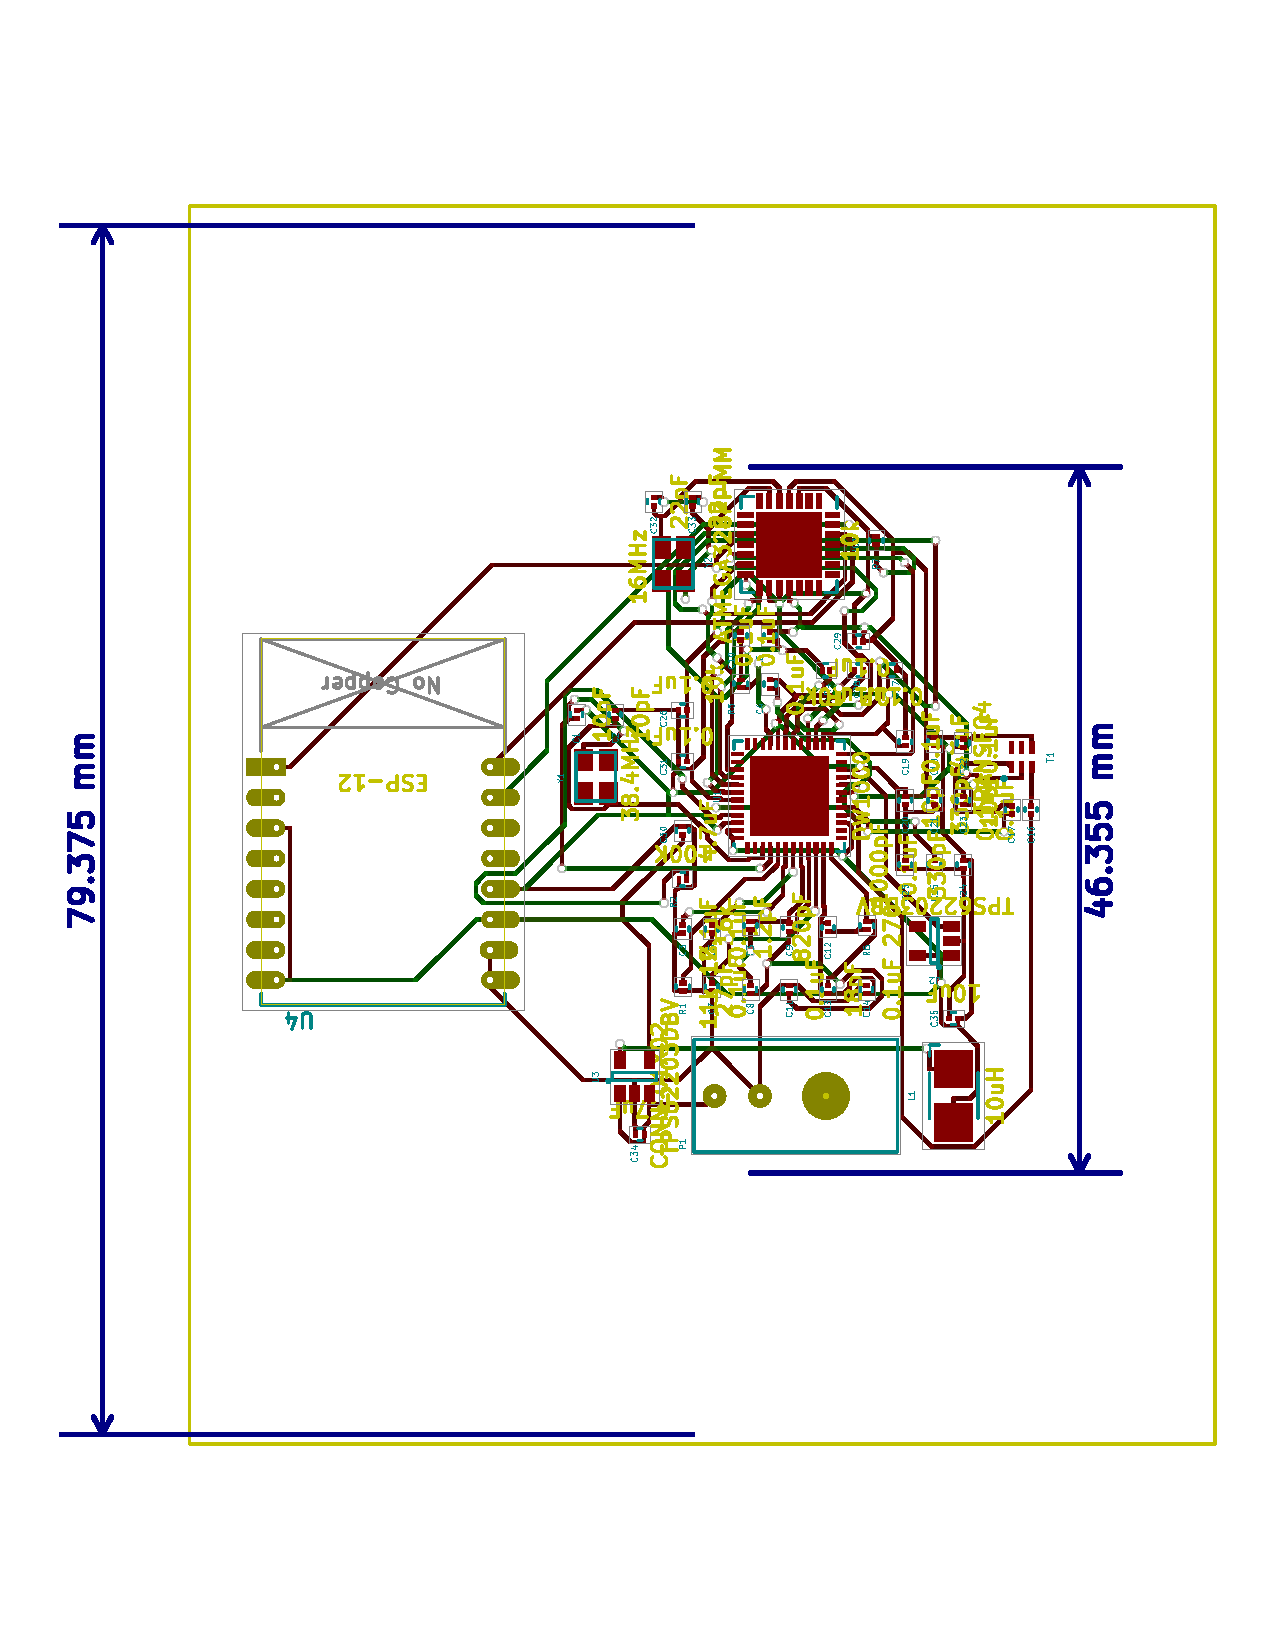
\includepdf[pages=-]{data/pcb-layout-ESP.pdf}

\newpage
\vspace*{\fill}
\begin{center}
\subsection*{Appendix F: Tag Bill of Materials and Unit Cost}
\end{center}
\vspace*{\fill}
\addcontentsline{toc}{section}{Appendix F: Tag Bill of Materials and Unit Cost}

\begin{landscape}
\begin{table}[]
\centering
\tiny
\caption{Tag Bill of Materials and Unit Cost Analysis}
\label{bom}
\begin{tabular}{llllllll}
\textbf{Ref}   & \textbf{Type} & \textbf{Value}             & \textbf{Footprint}              & \textbf{Part No. (Mouser default)}   & \textbf{Cost (US\$)} & \textbf{Outlay} & \textbf{Cost Outlay} \\
C4             & Capacitor     & 0.1uF                      & Capacitors\_SMD:C\_0201         & 81-GRM033R60J104KE19                 & 0.005                & 15000           & 75                   \\
C6             & Capacitor     & 0.1uF                      & Capacitors\_SMD:C\_0201         & 81-GRM033R60J104KE19                 & 0.005                & 15000           & 75                   \\
R2             & Resistor      & 100K                       & Resistors\_SMD:R\_0201          & 660-RK73H1HTTC1003F                  & 0.01                 & 15000           & 150                  \\
C31            & Capacitor     & 0.1uF                      & Capacitors\_SMD:C\_0201         & 81-GRM033R60J104KE19                 & 0.005                & 15000           & 75                   \\
C30            & Capacitor     & 4.7uF                      & Capacitors\_SMD:C\_0201         & 963-JMK063BJ474KP-F                  & 0.041                & 15000           & 615                  \\
C29            & Capacitor     & 0.1uF                      & Capacitors\_SMD:C\_0201         & 81-GRM033R60J104KE19                 & 0.005                & 15000           & 75                   \\
C28            & Capacitor     & 0.1uF                      & Capacitors\_SMD:C\_0201         & 81-GRM033R60J104KE19                 & 0.005                & 15000           & 75                   \\
C27            & Capacitor     & 0.1uF                      & Capacitors\_SMD:C\_0201         & 81-GRM033R60J104KE19                 & 0.005                & 15000           & 75                   \\
C26            & Capacitor     & 0.1uF                      & Capacitors\_SMD:C\_0201         & 81-GRM033R60J104KE19                 & 0.005                & 15000           & 75                   \\
C25            & Capacitor     & 1000pF                     & Capacitors\_SMD:C\_0201         & 81-GRM033R71E102KA1D                 & 0.004                & 15000           & 60                   \\
C24            & Capacitor     & 330pF                      & Capacitors\_SMD:C\_0201         & 81-GRM033R71E331KA1D                 & 0.004                & 15000           & 60                   \\
C23            & Capacitor     & 10pF                       & Capacitors\_SMD:C\_0201         & 81-GRM0335C1E100JA1D                 & 0.003                & 15000           & 45                   \\
C22            & Capacitor     & 0.1uF                      & Capacitors\_SMD:C\_0201         & 81-GRM033R60J104KE19                 & 0.005                & 15000           & 75                   \\
C21            & Capacitor     & 330pF                      & Capacitors\_SMD:C\_0201         & 81-GRM033R71E331KA1D                 & 0.004                & 15000           & 60                   \\
C20            & Capacitor     & 10pF                       & Capacitors\_SMD:C\_0201         & 81-GRM0335C1E100JA1D                 & 0.003                & 15000           & 45                   \\
C19            & Capacitor     & 0.1uF                      & Capacitors\_SMD:C\_0201         & 81-GRM033R60J104KE19                 & 0.005                & 15000           & 75                   \\
C18            & Capacitor     & 47uF                       & Capacitors\_SMD:C\_0201         & 581-TPSC476K016R0350                 & 0.206                & 15000           & 3090                 \\
C15            & Capacitor     & 0.1uF                      & Capacitors\_SMD:C\_0201         & 81-GRM033R60J104KE19                 & 0.005                & 15000           & 75                   \\
C17            & Capacitor     & 0.1uF                      & Capacitors\_SMD:C\_0201         & 81-GRM033R60J104KE19                 & 0.005                & 15000           & 75                   \\
C16            & Capacitor     & 0.1uF                      & Capacitors\_SMD:C\_0201         & 81-GRM033R60J104KE19                 & 0.005                & 15000           & 75                   \\
T1             & Transformer   & TRANSFO4                   & footprints:HHM1595A1            & 810-HHM1595A1                        & 0.362                & 15000           & 5430                 \\
C14            & Capacitor     & 0.1uF                      & Capacitors\_SMD:C\_0201         & 81-GRM033R60J104KE19                 & 0.005                & 15000           & 75                   \\
R6             & Resistor      & 270                        & Resistors\_SMD:R\_0201          & 667-ERJ-1GNF2700C                    & 0.005                & 15000           & 75                   \\
C12            & Capacitor     & 820pF                      & Capacitors\_SMD:C\_0201         & 81-GRM033R71E821KA1D                 & 0.004                & 15000           & 60                   \\
C13            & Capacitor     & 18pF                       & Capacitors\_SMD:C\_0201         & 581-02013A180GAT2A                   & 0.099                & 15000           & 1485                 \\
C11            & Capacitor     & 0.1uF                      & Capacitors\_SMD:C\_0201         & 81-GRM033R60J104KE19                 & 0.005                & 15000           & 75                   \\
C9             & Capacitor     & 1.2pF                      & Capacitors\_SMD:C\_0201         & 810-C0603C0G1E1R2BTQ                 & 0.02                 & 15000           & 300                  \\
R3             & Resistor      & 16k                        & Resistors\_SMD:R\_0201          & 667-ERJ-1GEJ163C                     & 0.004                & 15000           & 60                   \\
C8             & Capacitor     & 27pF                       & Capacitors\_SMD:C\_0201         & 81-GRM0335C1E270JA1D                 & 0.004                & 15000           & 60                   \\
C7             & Capacitor     & 0.1uF                      & Capacitors\_SMD:C\_0201         & 81-GRM033R60J104KE19                 & 0.005                & 15000           & 75                   \\
R1             & Resistor      & 11k 1\%                    & Resistors\_SMD:R\_0201          & 71-CRCW020111K0FKED                  & 0.026                & 15000           & 390                  \\
C5             & Capacitor     & 0.1uF                      & Capacitors\_SMD:C\_0201         & 81-GRM033R60J104KE19                 & 0.005                & 15000           & 75                   \\
C3             & Capacitor     & 0.1uF                      & Capacitors\_SMD:C\_0201         & 81-GRM033R60J104KE19                 & 0.005                & 15000           & 75                   \\
R4             & Resistor      & 10k                        & Resistors\_SMD:R\_0201          & 603-RC0201FR-0710KL                  & 0.004                & 15000           & 60                   \\
R5             & Resistor      & 10k                        & Resistors\_SMD:R\_0201          & 603-RC0201FR-0710KL                  & 0.004                & 15000           & 60                   \\
C2             & Capacitor     & 10pF                       & Capacitors\_SMD:C\_0201         & 81-GRM0335C1E100JA1D                 & 0.003                & 15000           & 45                   \\
C1             & Capacitor     & 10pF                       & Capacitors\_SMD:C\_0201         & 81-GRM0335C1E100JA1D                 & 0.003                & 15000           & 45                   \\
Y1             & Crystal       & 38.4MHz                    & Crystals:FA238-TSX3225          & ABM10-165-38.400MHz-T3               & 0.667                & 15000           & 10005                \\
C10            & Capacitor     & 0.1uF                      & Capacitors\_SMD:C\_0201         & 81-GRM033R60J104KE19                 & 0.005                & 15000           & 75                   \\
U1             & Transciever   & DW1000                     & Housings\_DFN\_QFN:QFN-48       & 1479-1001-2-ND                       & 8.8726               & 15000           & 133089               \\
U2             & DC-DC         & TPS62203DBV                & SMD:SOT-23-5                    & 595-TPS62203DBVR                     & 0.542                & 15000           & 8130                 \\
U3             & DC-DC         & TPS62203DBV                & SMD:SOT-23-5                    & 595-TPS62203DBVR                     & 0.542                & 15000           & 8130                 \\
C34            & Capacitor     & 4.7uF                      & Capacitors\_SMD:C\_0201         & 963-JMK063BJ474KP-F                  & 0.041                & 15000           & 615                  \\
L1             & Inductor      & 10uH                       & Inductors:Inductor\_1212        & 81-LQH3NPN100MM0L                    & 0.132                & 15000           & 1980                 \\
C35            & Capacitor     & 10uF                       & Capacitors\_SMD:C\_0201         & 80-T491C106K016                      & 0.102                & 15000           & 1530                 \\
P1             & Connector     & CONN\_01X02                & Connectors\_Molex               & See note.                            & 0.5                  & 15000           & 7500                 \\
P2             & Antenna       & Antenna                    & PCB Chip Antenna                & 963-AH086M555003-T                   & 0.803                & 15000           & 12045                \\
IC1            & Micro.        & ATMEGA328P-MM              & DFN\_QFN:QFN-28                 & 556-ATMEGA328P-MMH                   & 1.89                 & 15000           & 28350                \\
R7             & Resistor      & 10k                        & Resistors\_SMD:R\_0201          & 603-RC0201FR-0710KL                  & 0.004                & 15000           & 60                   \\
Y2             & Crystal       & 16MHz                      & Crystals:crystal\_FA238-TSX3225 & 732-TX325-16F09Z-AC3                 & 0.278                & 15000           & 4170                 \\
C32            & Capacitor     & 22pF                       & Capacitors\_SMD:C\_0201         & 810-C0603C0G1H220J                   & 0.004                & 15000           & 60                   \\
C33            & Capacitor     & 22pF                       & Capacitors\_SMD:C\_0201         & 810-C0603C0G1H220J                   & 0.004                & 15000           & 60                   \\
               &               &                            &                                 & \textbf{Total Capital Outlay (ZAR):} &                      &                 & \textbf{3558254.88}  \\
               &               &                            &                                 & \textbf{Unit Cost (ZAR):}            &                      &                 & \textbf{237.216992}  \\
               &               &                            &                                 &                                      &                      &                 &                      \\
\textbf{Notes} &               &                            &                                 &                                      &                      &                 &                      \\
P1             & Connector     & Part No.: Diff. Footprint. &                                 &                                      &                      &                 &                      \\
C35            & Capacitor     & Footprint: 2412            &                                 &                                      &                      &                 &                      \\
U1             & Transciever   & Supplier: Digikey          &                                 &                                      &                      &                 &                     
\end{tabular}
\end{table}
\end{landscape}

\newpage
\vspace*{\fill}
\begin{center}
\subsection*{Appendix G1: Beacon Structural Schematics}
\end{center}
\vspace*{\fill}
\addcontentsline{toc}{section}{Appendix G1: Beacon Structural Schematics}

\newpage
\begin{center}
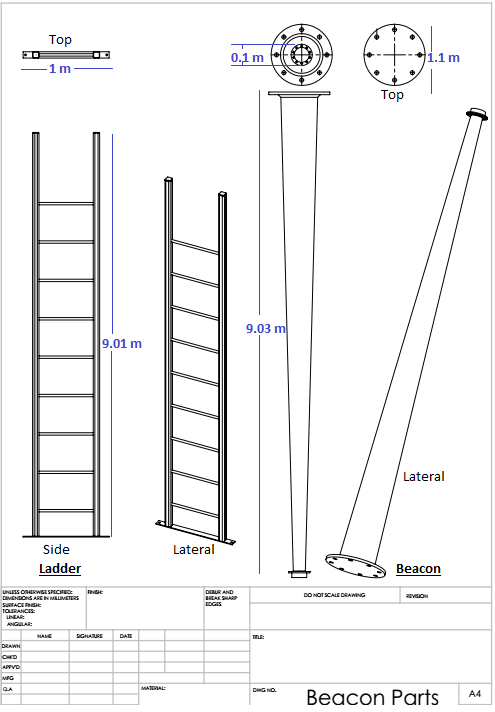
\includegraphics[scale=1.3]{data/mechanical/a1.png}
\end{center}

\newpage
\vspace*{\fill}
\begin{center}
\subsection*{Appendix G2: Tag Case Schematics}
\end{center}
\vspace*{\fill}
\addcontentsline{toc}{section}{Appendix G2: Tag Case Schematics}

\newpage
\begin{center}
\includegraphics[scale=1.3]{data/mechanical/a2.png}
\end{center}

\newpage
\vspace*{\fill}
\begin{center}
\subsection*{Appendix H: Beacon Placement on UCT Upper Campus}
\end{center}
\vspace*{\fill}
\addcontentsline{toc}{section}{Appendix H: Beacon Placement on UCT Upper Campus}

\newpage
\begin{figure}[H]
\begin{center}
\includegraphics[scale=0.3]{data/mechanical/8.png}
\caption{UCT Upper Campus parking areas.}
\label{fig:mech-8}
\end{center}
\end{figure}

\begin{figure}[H]
\begin{center}
\includegraphics[scale=0.5]{data/mechanical/9.jpg}
\caption{Beacon placement.}
\label{fig:mech-9}
\end{center}
\end{figure}

%######################References######################
\newpage
%\input{"\homedir references.tex"} %manual references

\bibliography{bibliography}
\bibliographystyle{ieeetran}
\addcontentsline{toc}{section}{References}

\end{document}

%----------------------------------------------------------------------------


